\chapter{Experimental Findings}
The following chapter will give an overview of the data obtained from the survey, which was conducted before running the experiment.
Later, an overview of the data obtained from the experiment is explained along with some feedback received from the participants.

\section{Findings from the Pre-Survey}
The survey had 199 participants. Participants were not given any incentives to participate. After filtering out spurious and half-filled entries, 189 entries are used for the data analysis. In the following paragraphs, information obtained in the survey will be introduced.

Out of the total
participants 63.64\% are male and 36.36\% are female. The mean year of birth was found to be 1985. The demographics of the participants is illustrated in Table \ref{tab:demo}. On the education level 2.53\% have not completed high school, 9.60\% have completed high school, 5.05\% have gone to some college, 28.79\% have obtained their bachelors degree, 39.90\% have obtained their masters degrees and 14.14\% have obtained their Phds. About the employment of the participants, 51.52\% are full time employees, 6.06\% are part time employed, 6.06\% are unemployed and looking for work, 1.52\% are unemployed and not looking for work, 0.51\% are retired and 41.92\% are students. None of the participants are disabled. 


Figure \ref{fig:pre_q7} shows the frequency of mobile usage among the population. It is observed that the majority of the people use their phones 36-70 times a day.

\begin{figure}[htp]
\subtop[Applications in the Mobile Phone\label{fig:pre_6}]{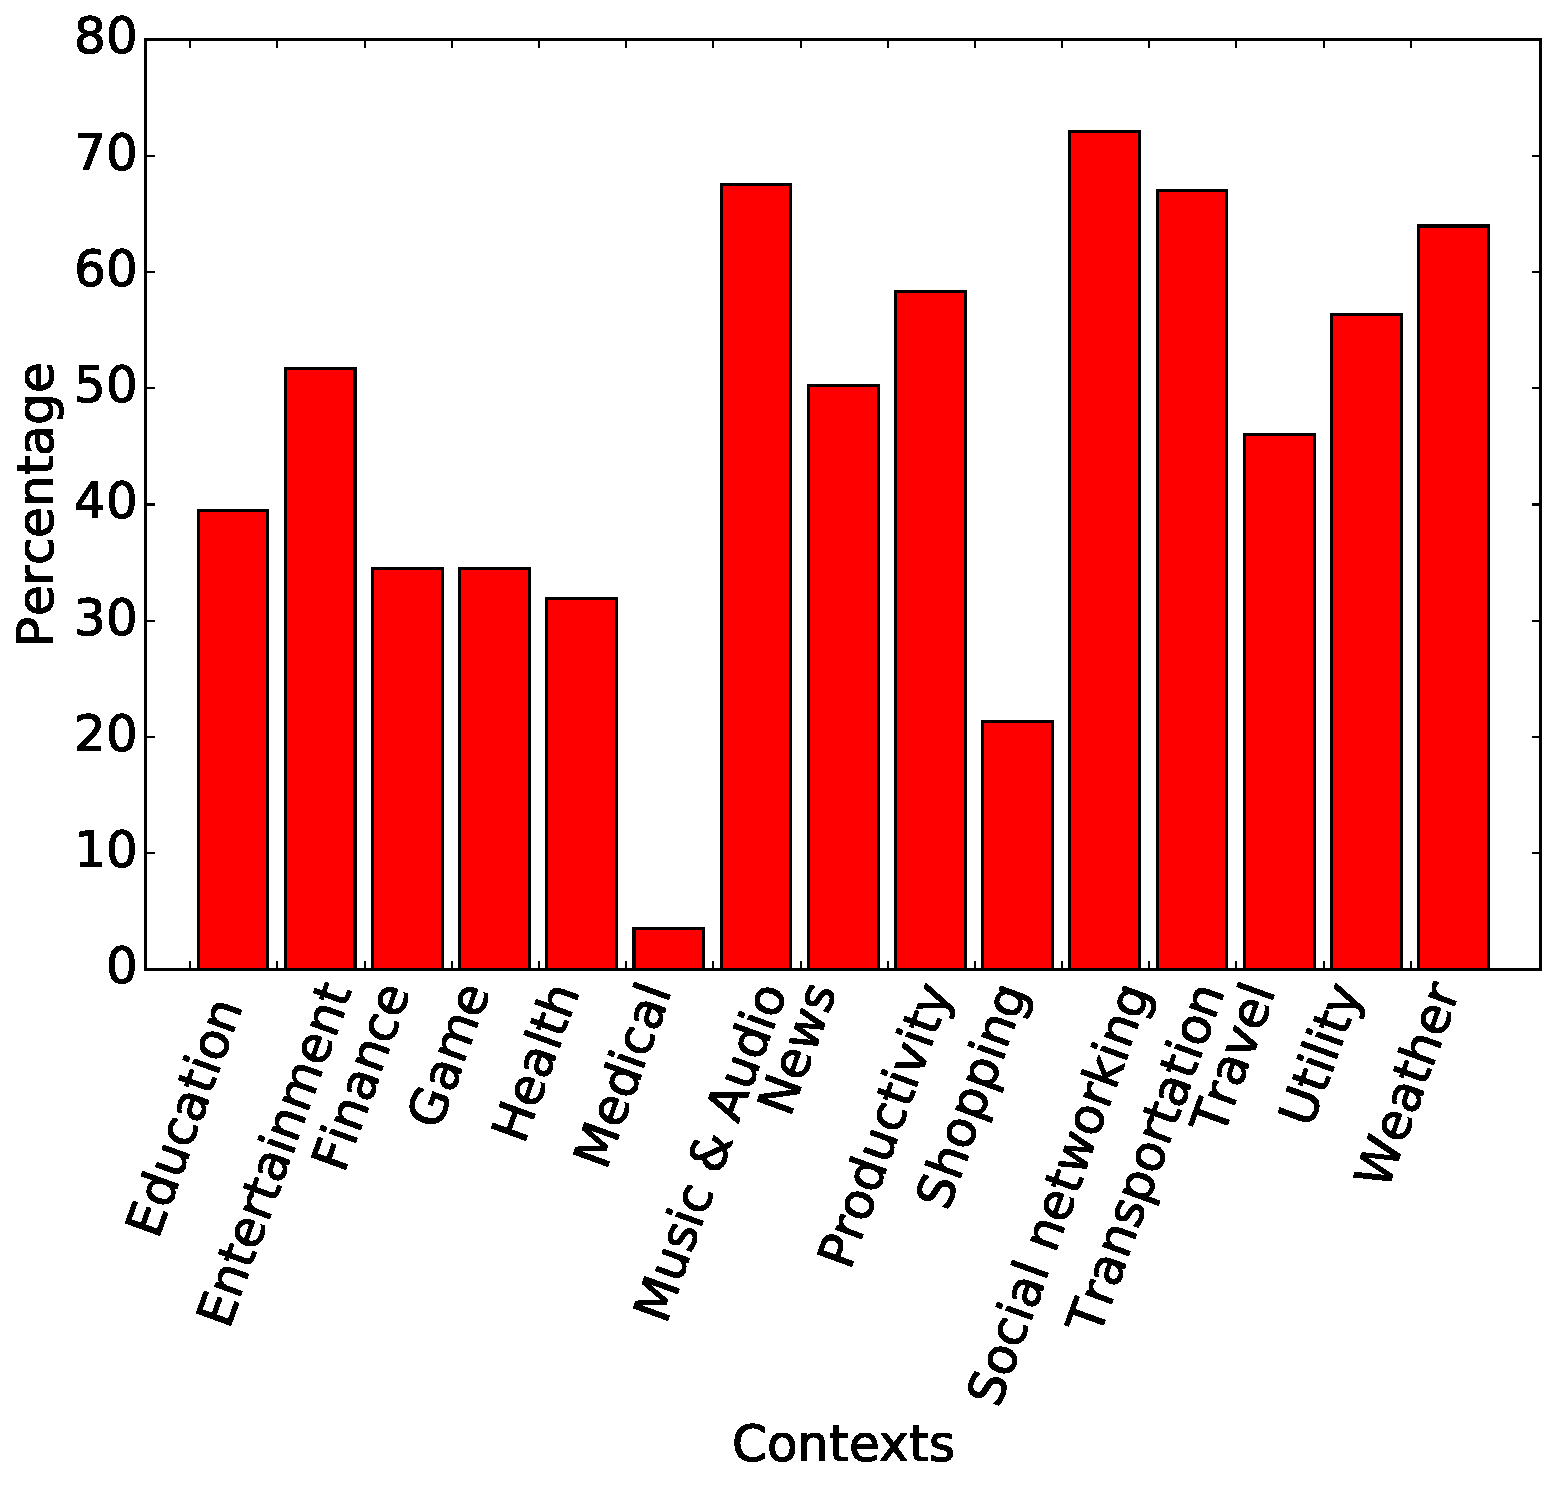
\includegraphics[width=0.45\linewidth]{./images/pre_6}}\hspace{1em}
\subtop[Incentives\label{fig:pre_q15}]{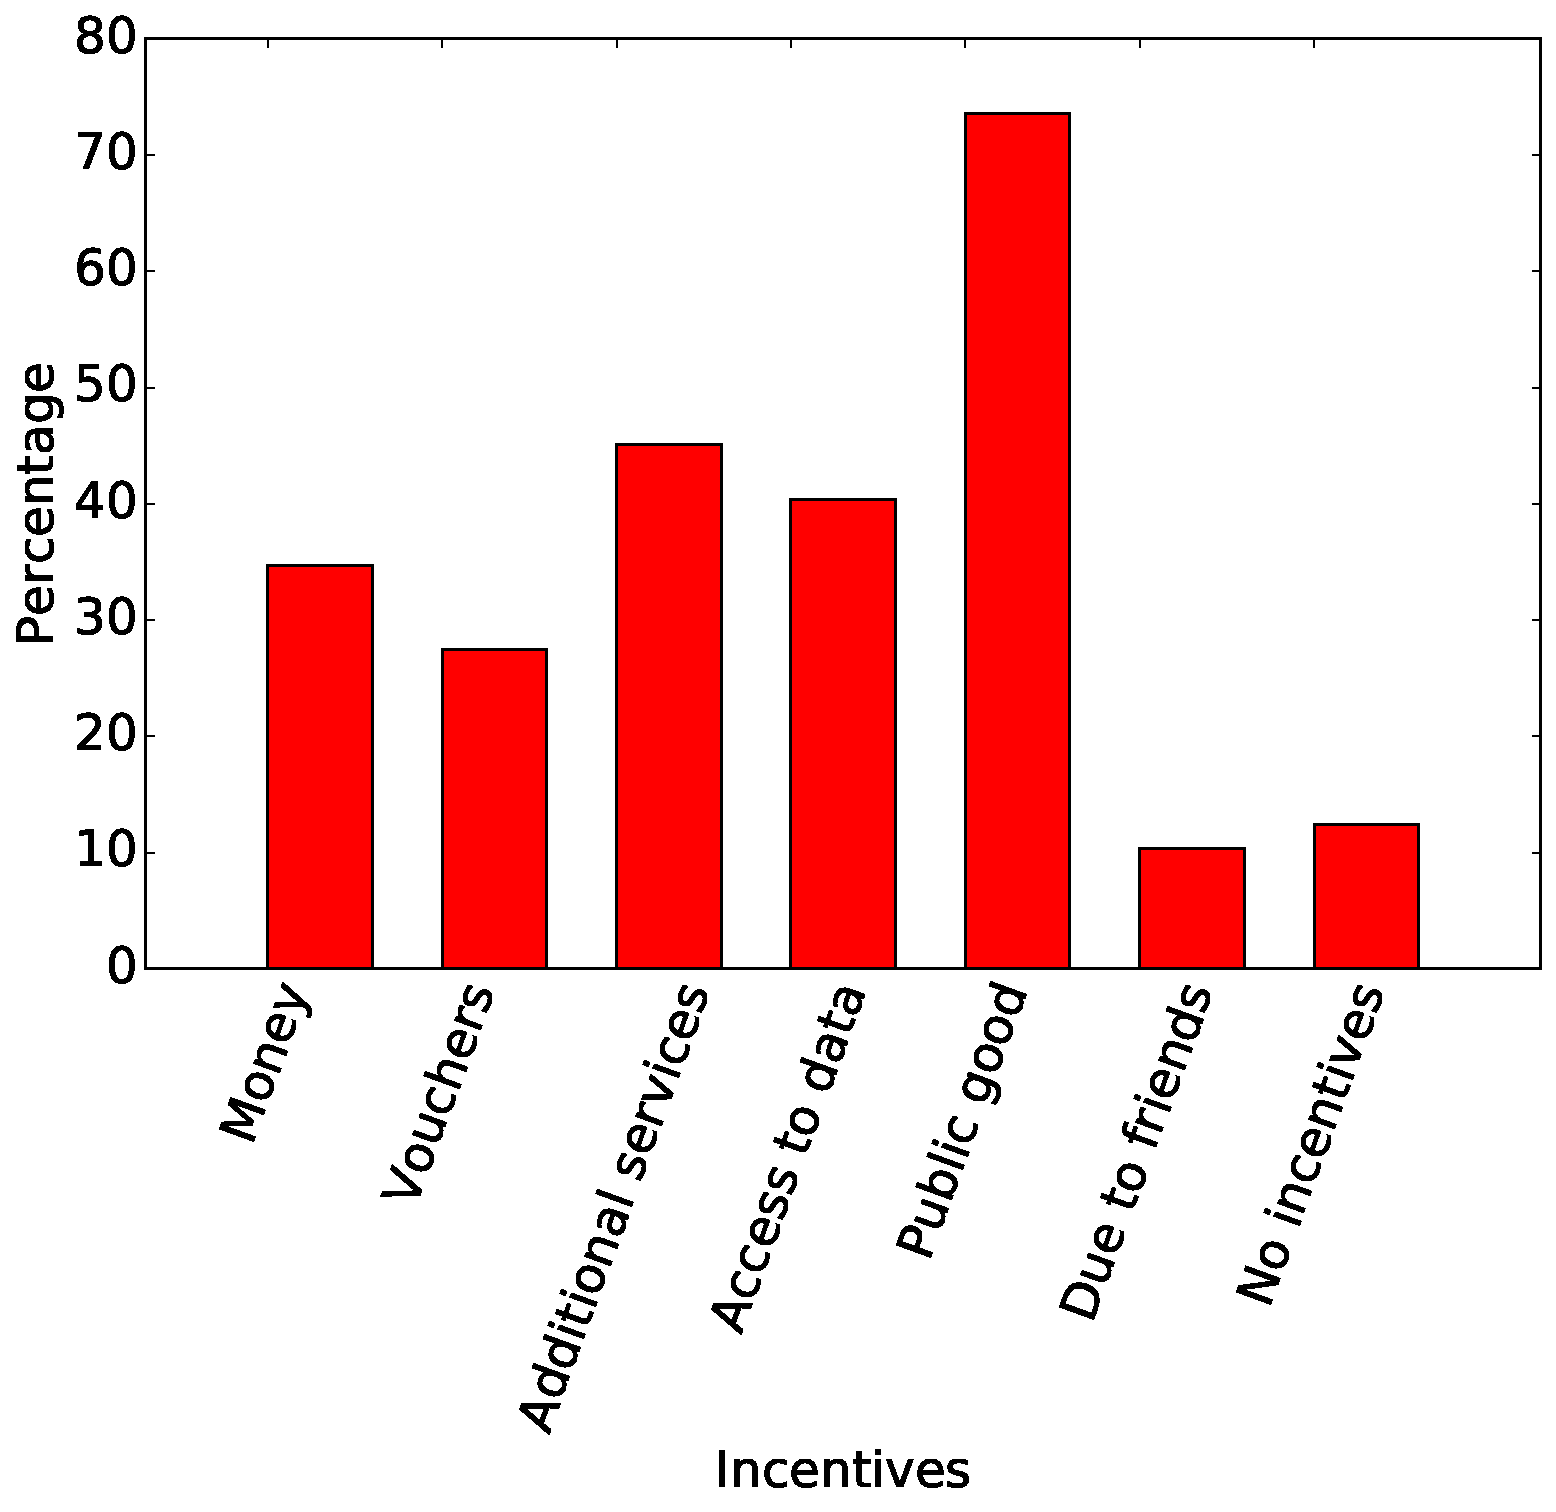
\includegraphics[width=0.45\linewidth]{./images/pre_incentives}}\newline
\centering
\subtop[Frequency of Mobile Phone Usage\label{fig:pre_q7}]{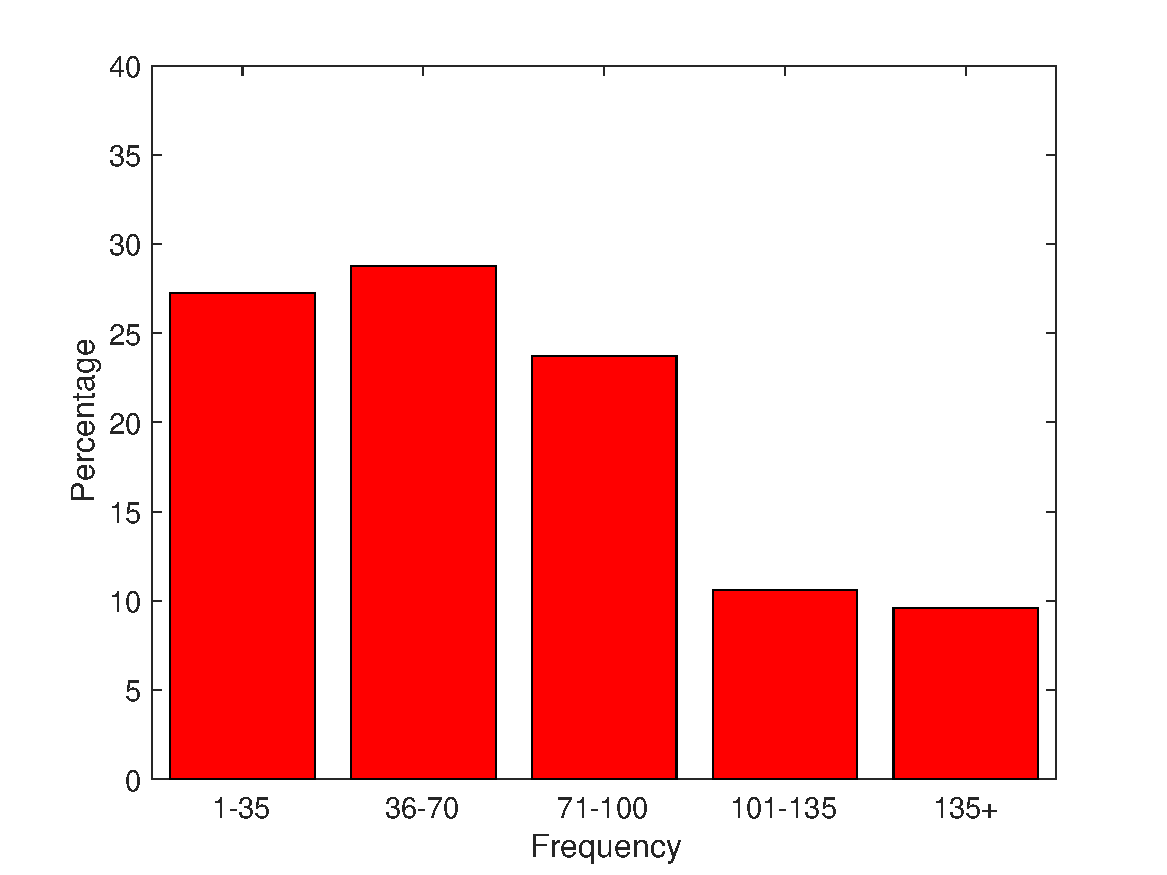
\includegraphics[width=0.45\linewidth]{./images/pre_q7}}

\caption{Table Schemas}
\label{fig:s3}
\end{figure}

Figure \ref{fig:pre_6} depicts the percentage of users who have different applications on their mobile phones. Is it observed that the applications which are installed the most are music and audio, social networking, transportation and weather applications with 67.51\%, 72.08\%, 67.01\% and 63.96\% of users having them installed respectively.

Figure \ref{fig:pre_q15} shows the percentage of users who would give data for each incentive indicated. As it can be observed, 73.58\% of users would give data for public good which is the most chosen option. The least popular reasons to share data are \textit{"Due to friends"} and \textit{"No incentives"}. 34.72\% of users would accept \textit{"Money"} as an incentive, 27.46\% would accept \textit{"Vouchers"}, 45.08\% would accept \textit{"Additional services"}, 40.41\% would accept \textit{"Free access to data"}. This shows that money is possibly not the only incentive that can be used to incentivize users to share more data.


\begin{figure}[htp]
\subtop[Level of concern of privacy for mobile sensor data\label{fig:pre_8}]{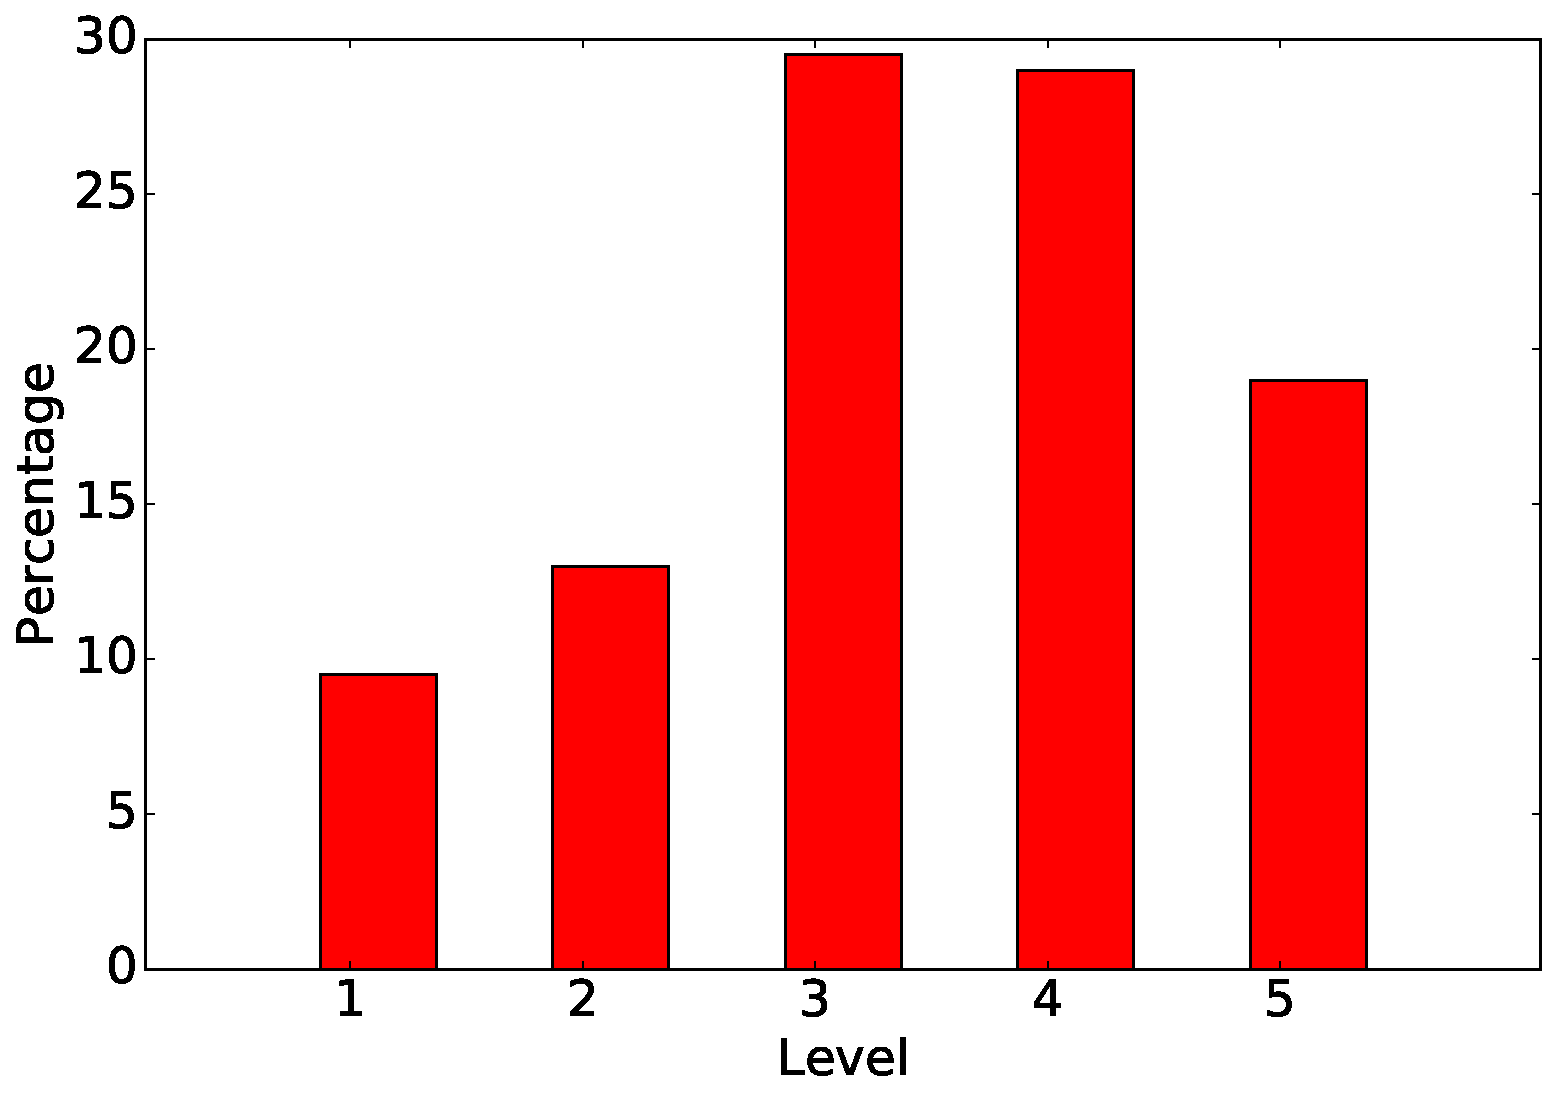
\includegraphics[width=0.5\linewidth]{./images/pre_mobile_concern}}\hspace{1em}
\subtop[Importance of sensor type for data sharing\label{fig:pre_10}]{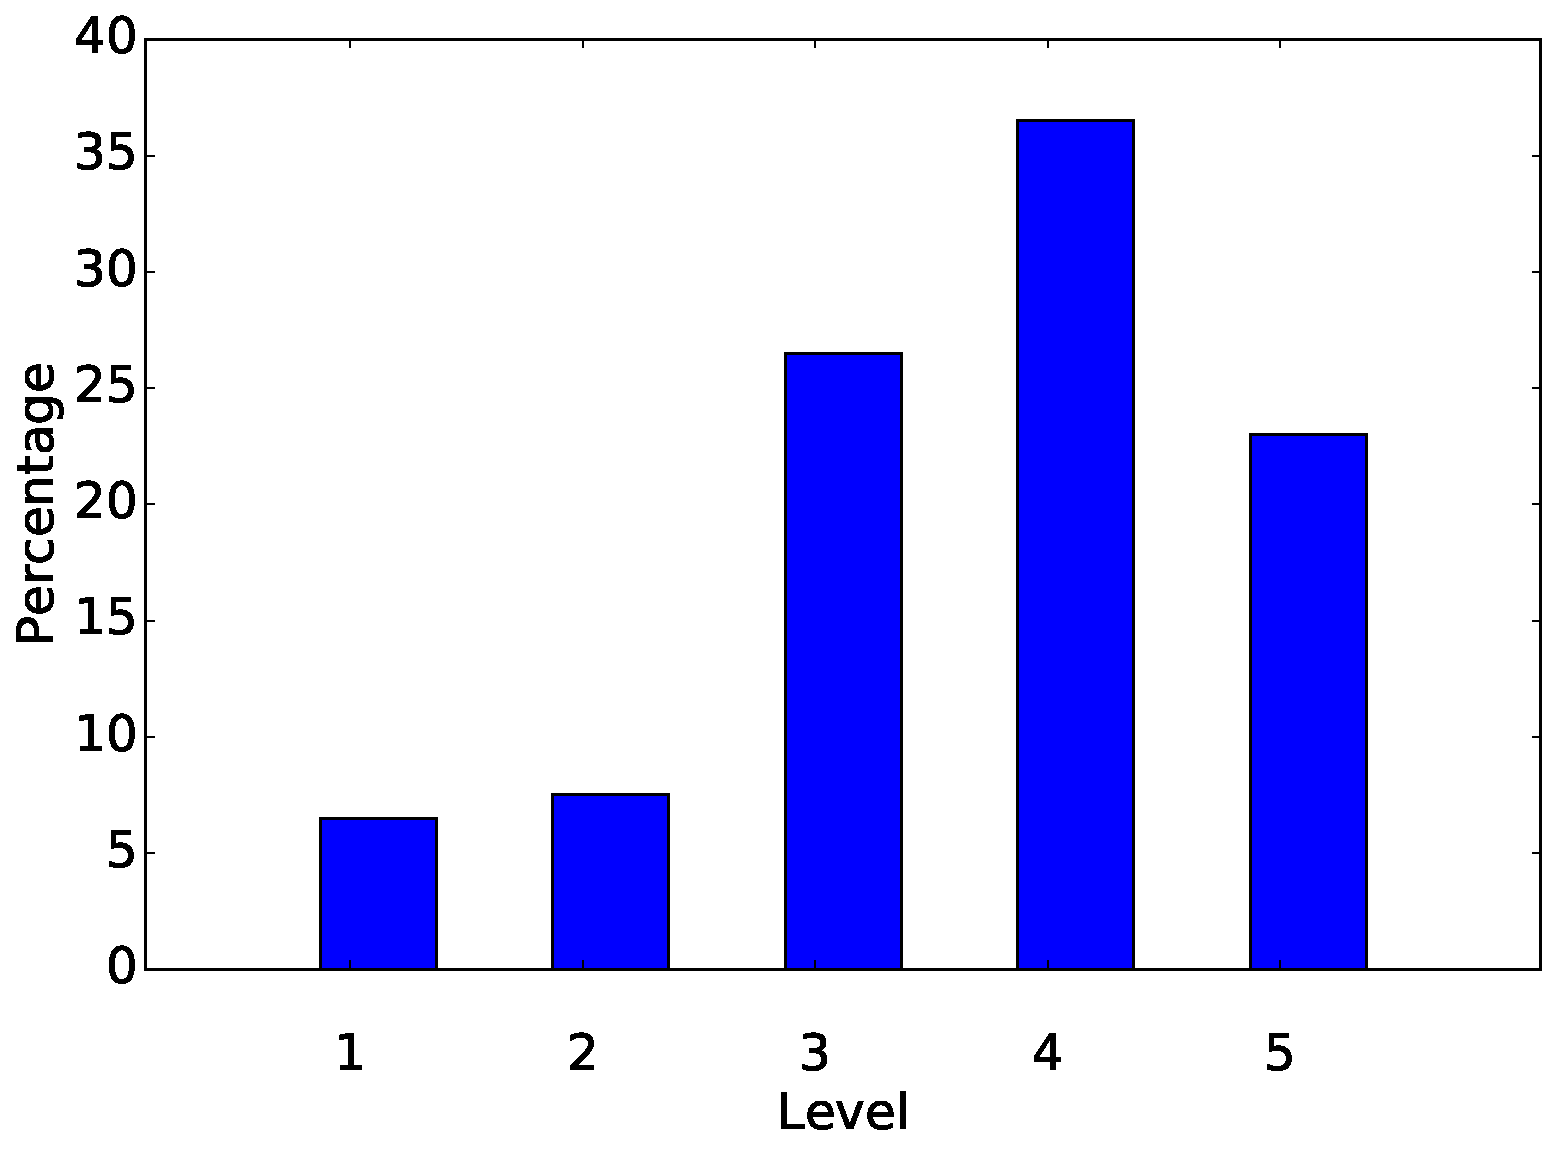
\includegraphics[width=0.5\linewidth]{./images/pre_se_imp}}\newline
\subtop[Importance of stakeholder type for data sharing\label{fig:pre_12}]{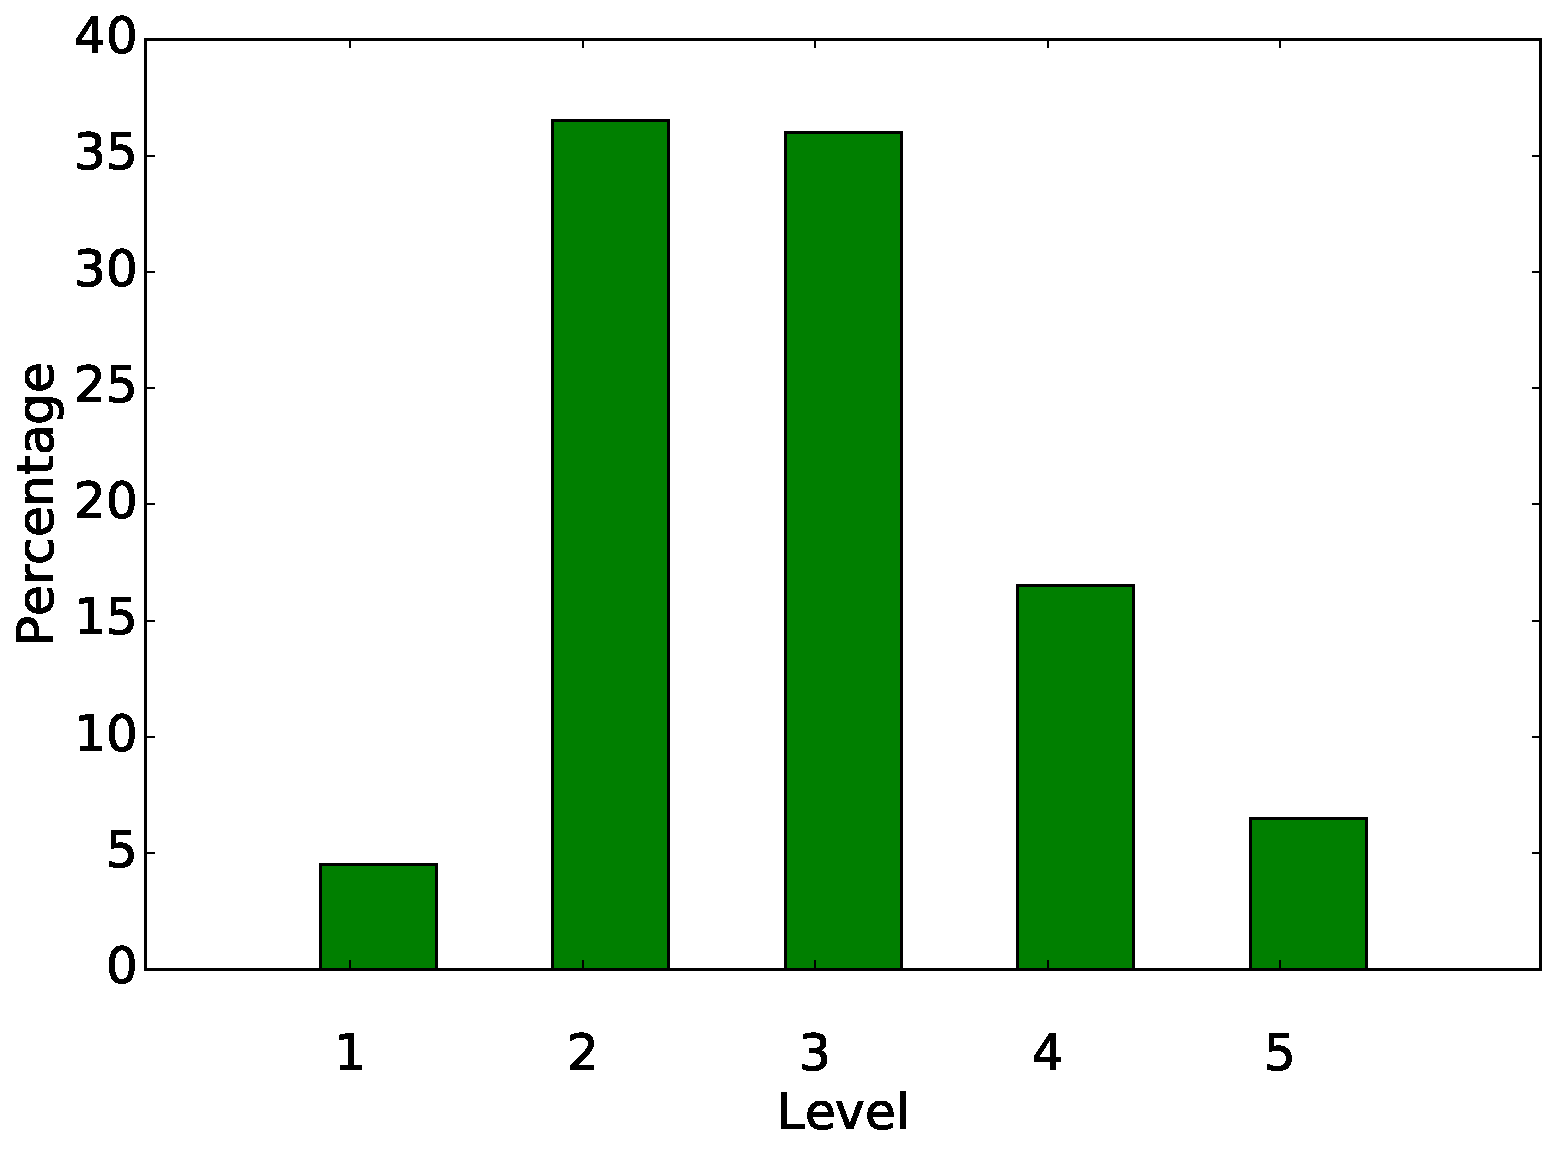
\includegraphics[width=0.5\linewidth]{./images/pre_st_imp}}\hspace{1em}
\subtop[Importance of context type for data sharing\label{fig:pre_14}]{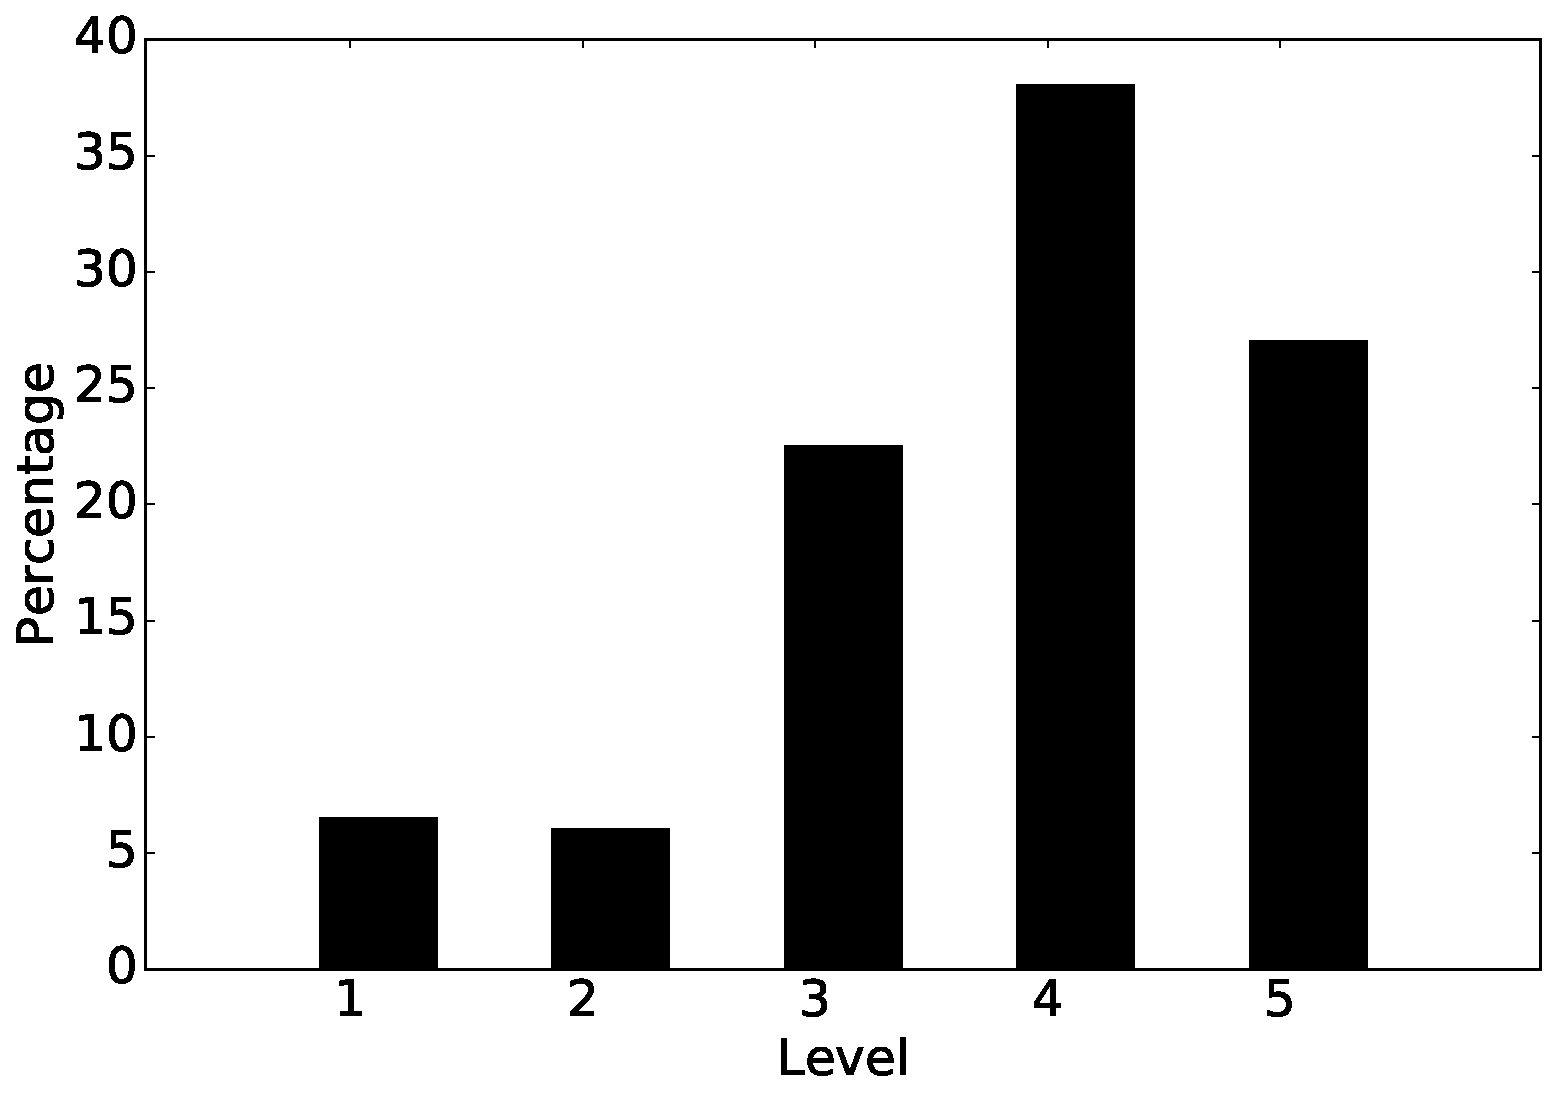
\includegraphics[width=0.5\linewidth]{./images/pre_co_imp}}
\caption{Figures for mobile privacy concern, importance of sensors, importance of stakeholders and importance of contexts for data sharing}
\label{fig:st3}
\end{figure}

Figure \ref{fig:pre_8} depicts the percentage of people who have different levels of concern for the privacy of their mobile sensor data. Level 1 corresponds to \textit{"Not at all concerned"} and level 5 to \textit{"Extremely concerned"}. As seen, 77.5\% of users are concerned to a level of 3 and above and 22.5\% of users are concerned to a level of 1 and 2 together. This shows that most users are at least moderately concerned about the privacy of their mobile sensor data.

Figure \ref{fig:pre_10} depicts the importance of the sensor type for whom mobile sensor data is shared. Level 1 corresponds to \textit{"Not at all important"} and level 5 to \textit{"Extremely important"}. As seen, 36.5\% of users care to a level of 4 and 86\% of users care to a level of 3 and above. Similarly, Figure \ref{fig:pre_12} depicts the importance of the stakeholder type to which data is shared. 36\% and 36.50\% of users find the stakeholder important to a level of 4 and 5 respectively and 89\% of users find the importance of stakeholder to a level 3 and above. Figure \ref{fig:pre_14} shows the importance of the context of application, for which mobile sensor data is shared. 38\% of users find the importance of the context of application to a level of 4 and 87.5\% of users find the importance of the context of application to be of level 3 and above.

\begin{figure}[htp]
\subtop[Average intrusion of sensors\label{fig:pre_9}]{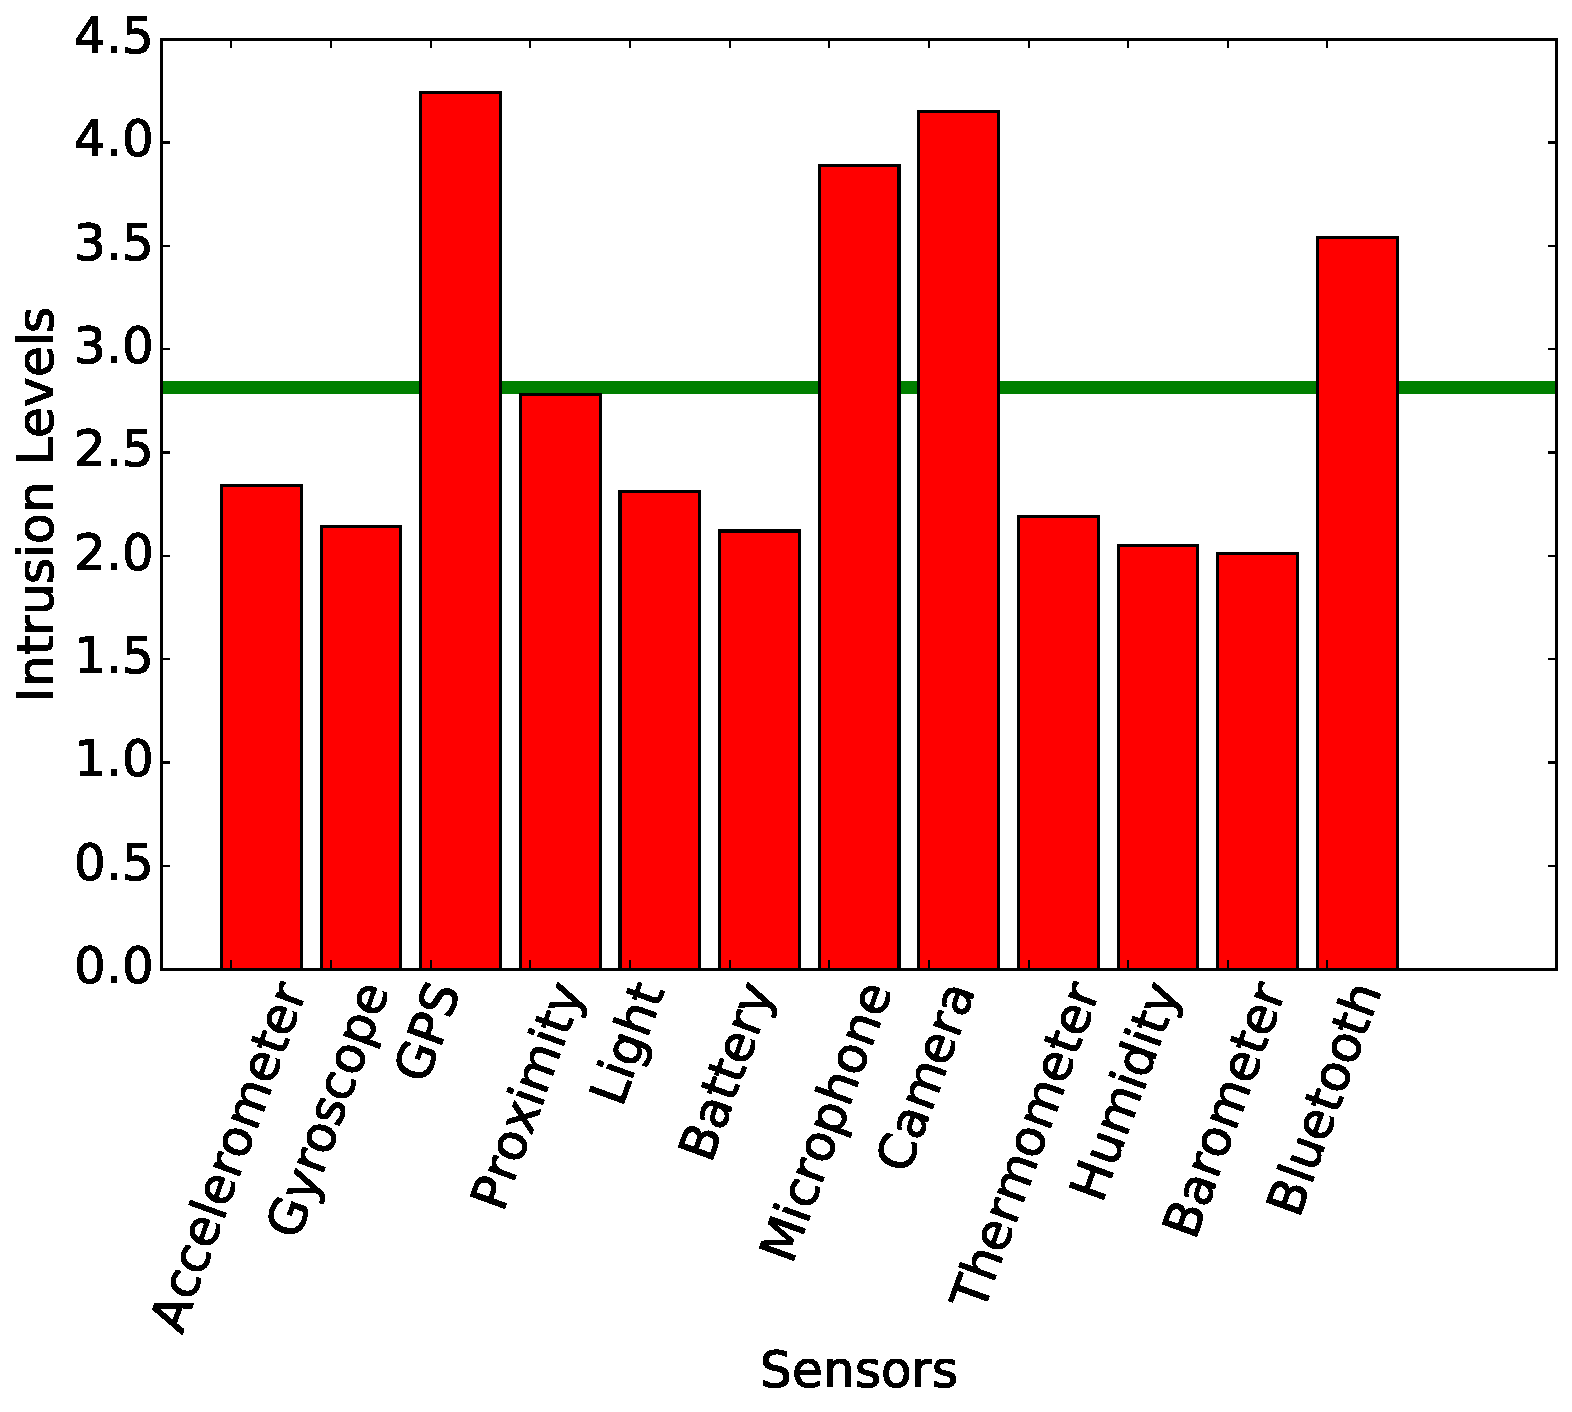
\includegraphics[width=0.5\linewidth]{./images/pre_se}}\hspace{1em}
\subtop[Standard deviation of sensor intrusions\label{fig:pre_9_sd}]{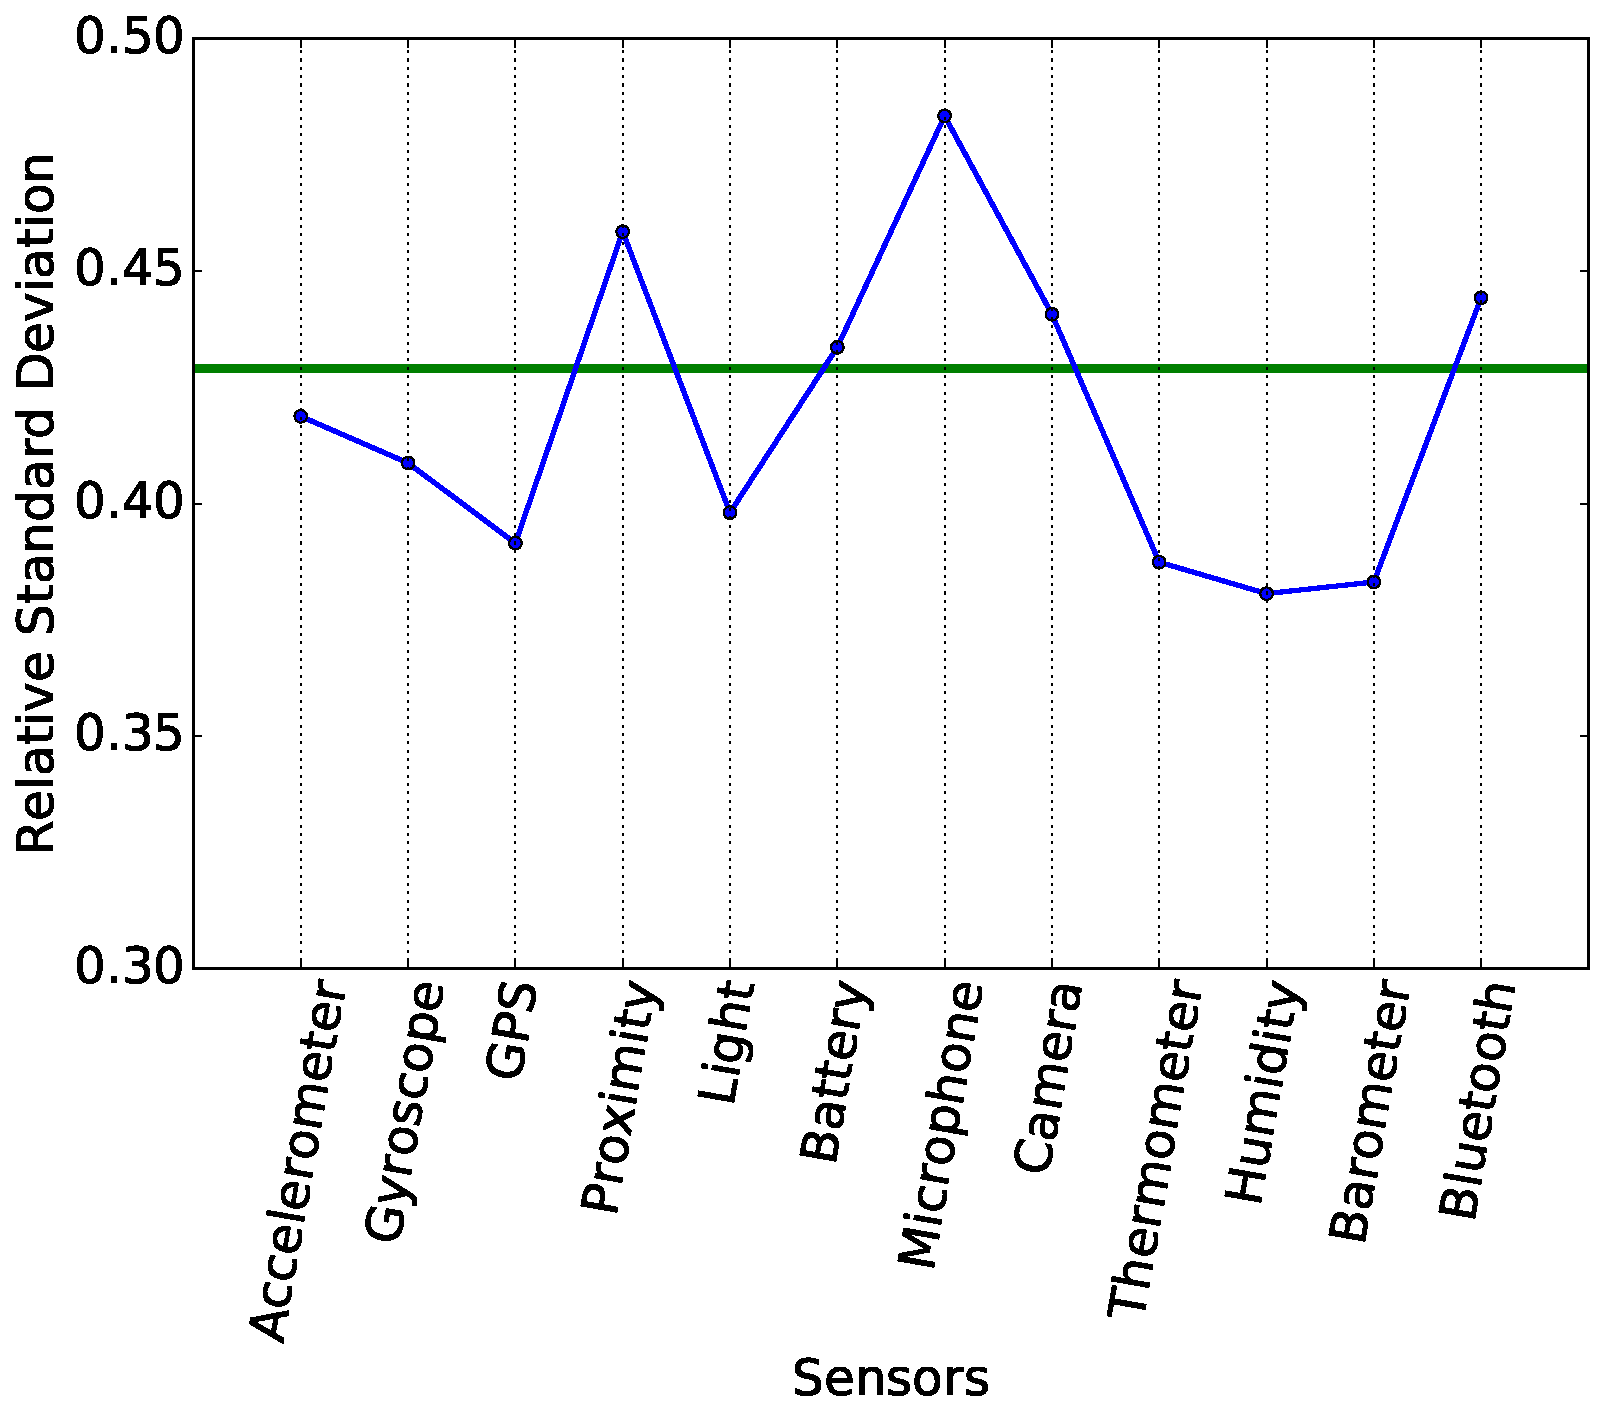
\includegraphics[width=0.5\linewidth]{./images/pre_se_sd}}\newline
\subtop[Average intrusion of stakeholders\label{fig:pre_11}]{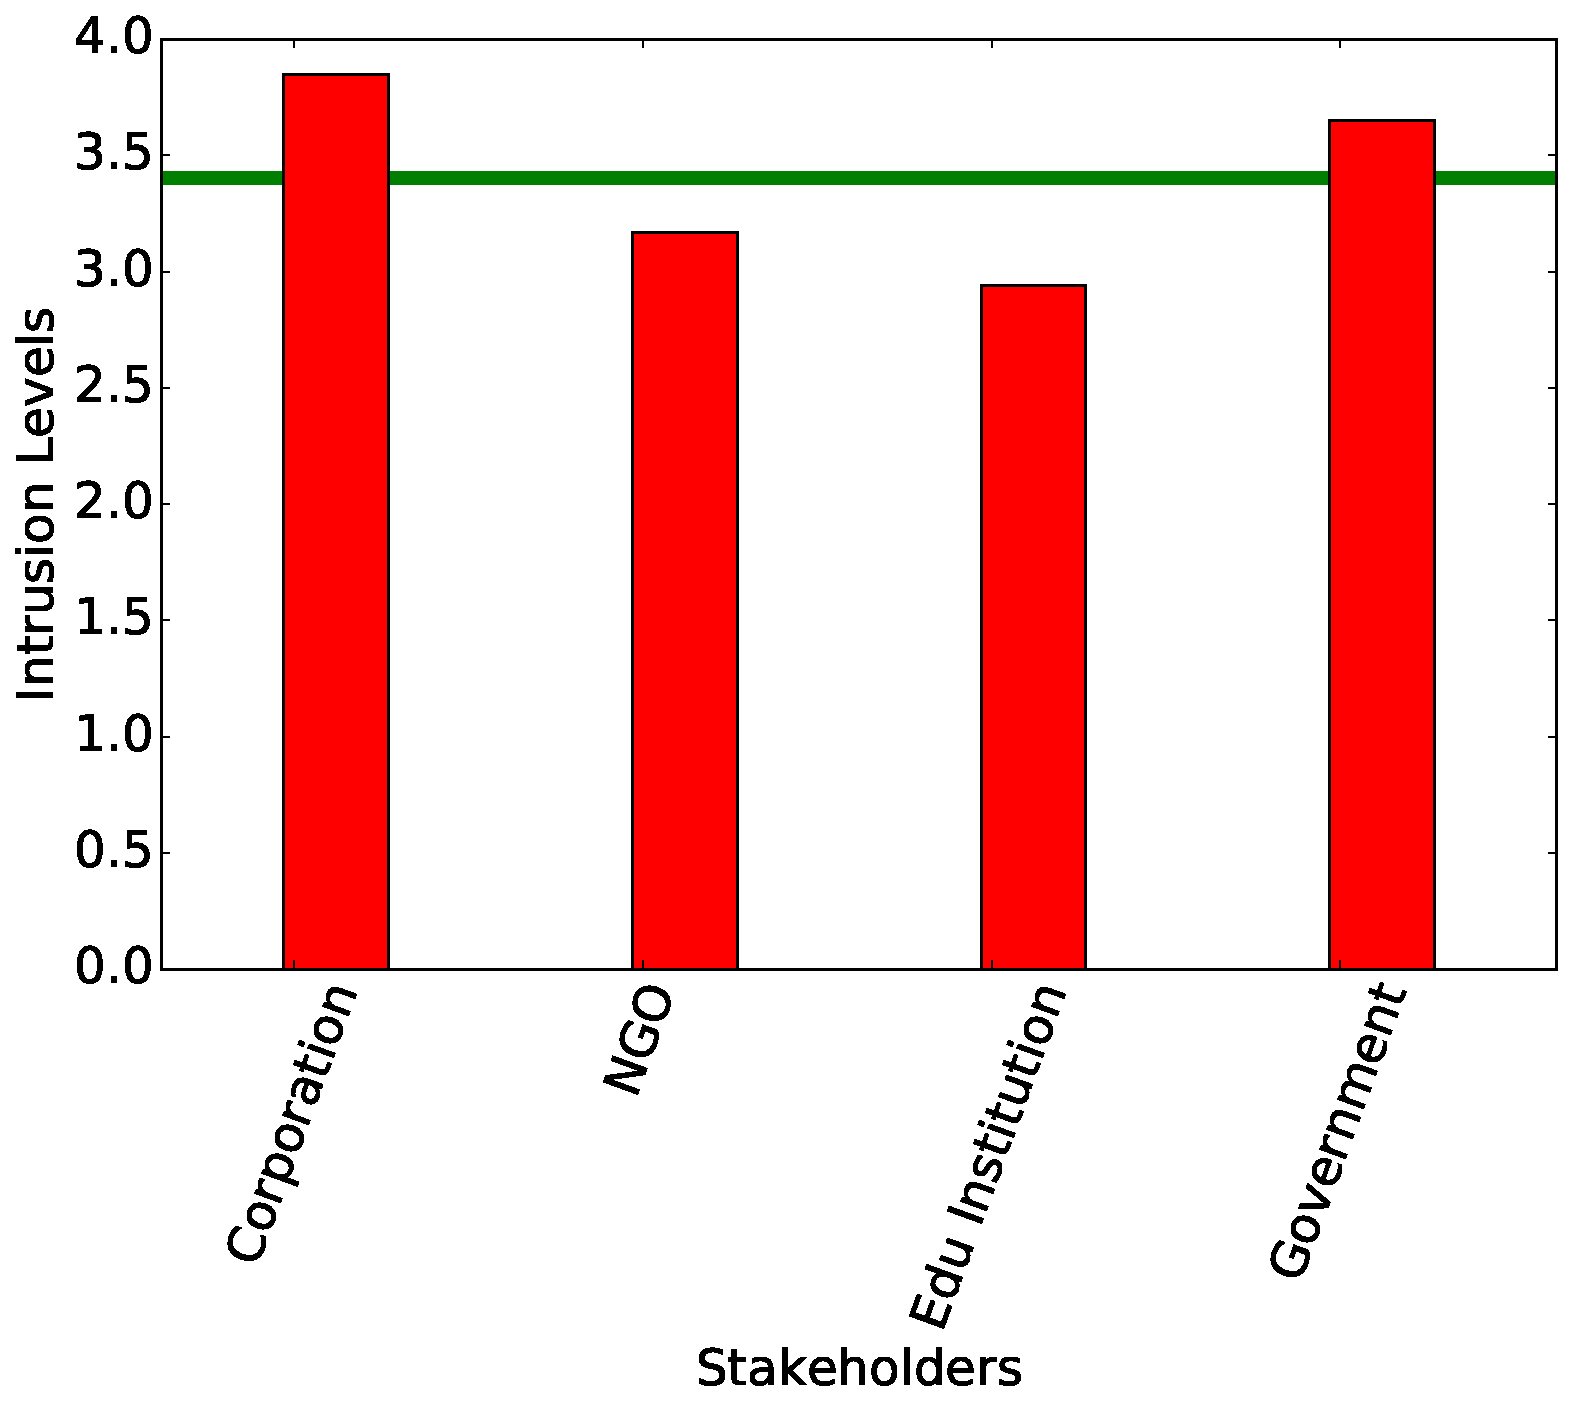
\includegraphics[width=0.5\linewidth]{./images/pre_st}}\hspace{1em}
\subtop[Standard deviation of stakeholder intrusions\label{fig:pre_11_sd}]{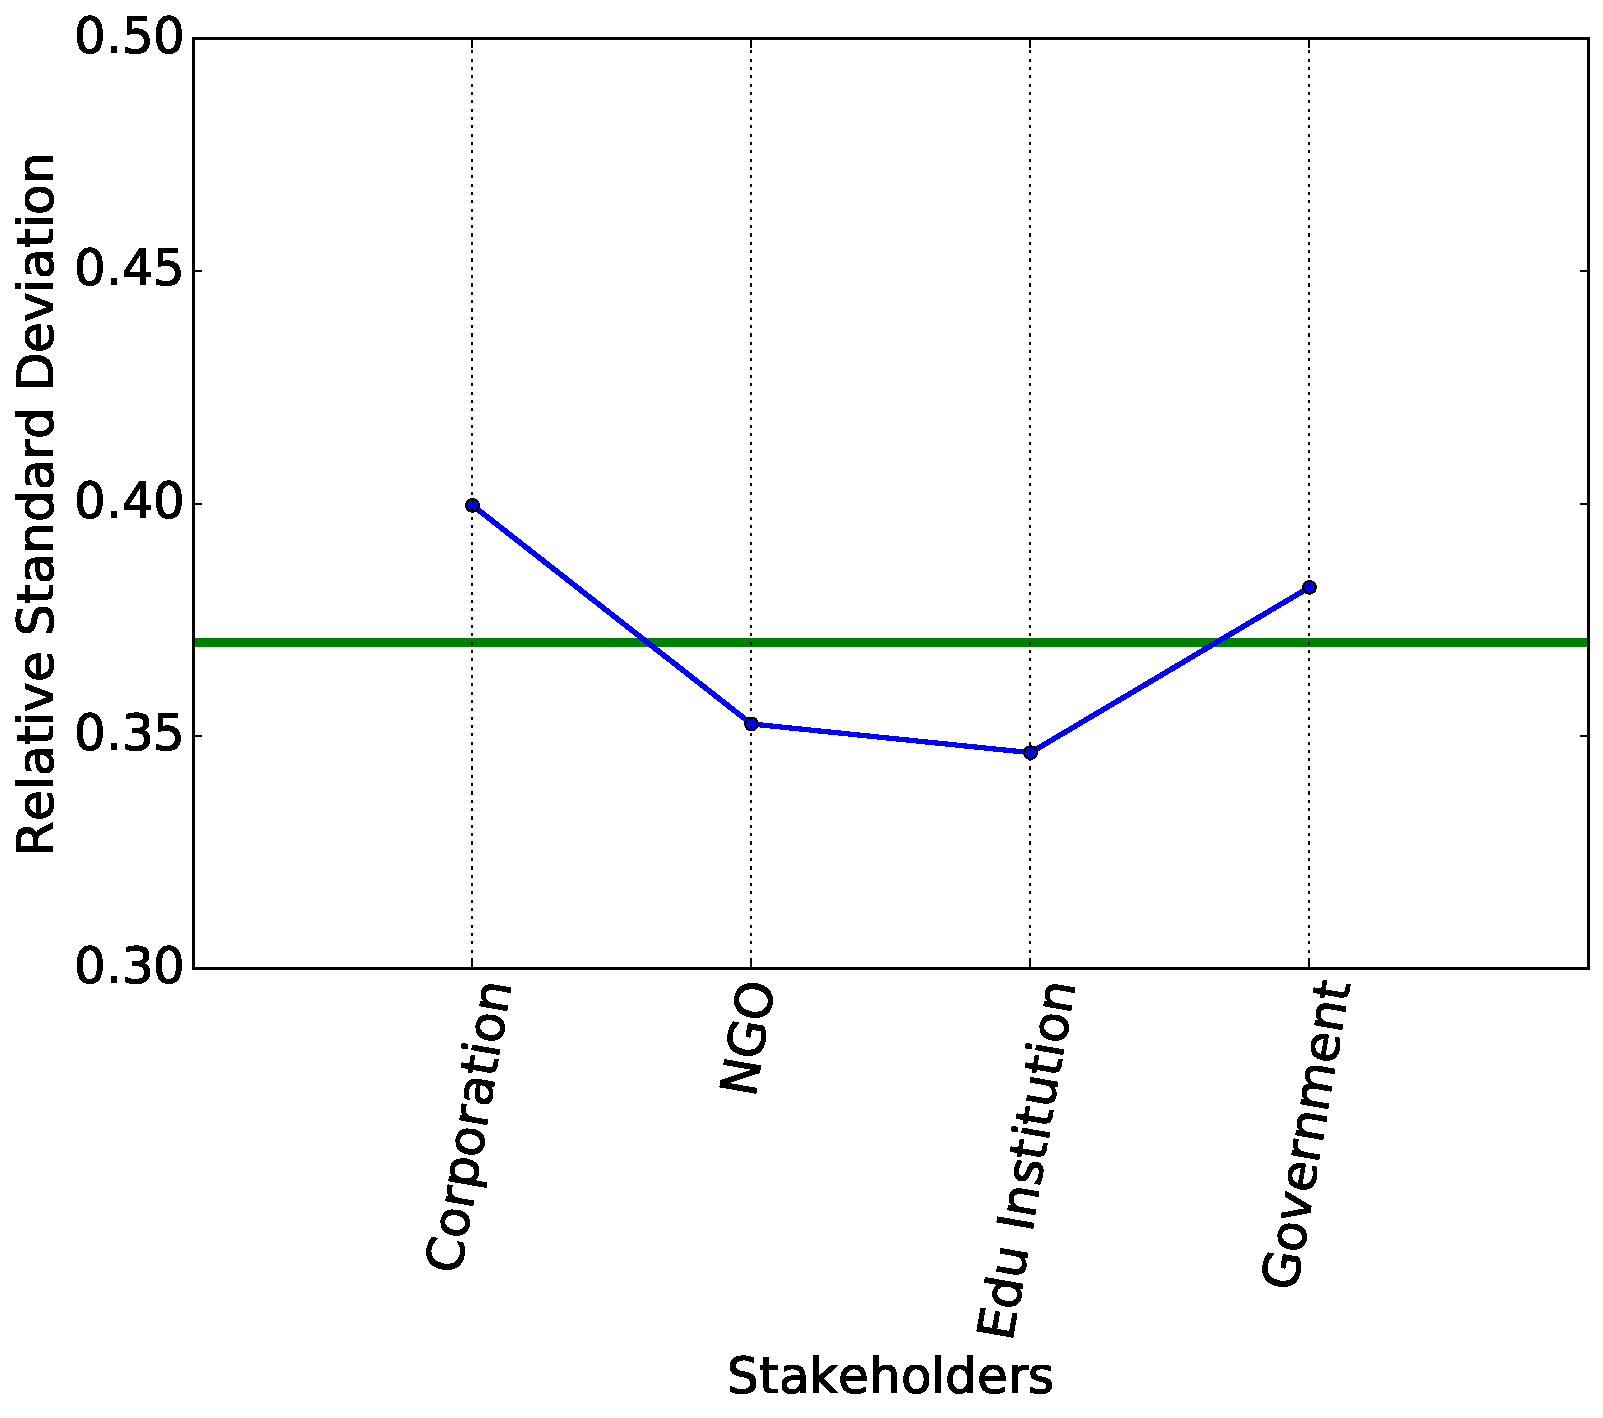
\includegraphics[width=0.5\linewidth]{./images/pre_st_sd}}\newline
\subtop[Average intrusion of contexts\label{fig:pre_13}]{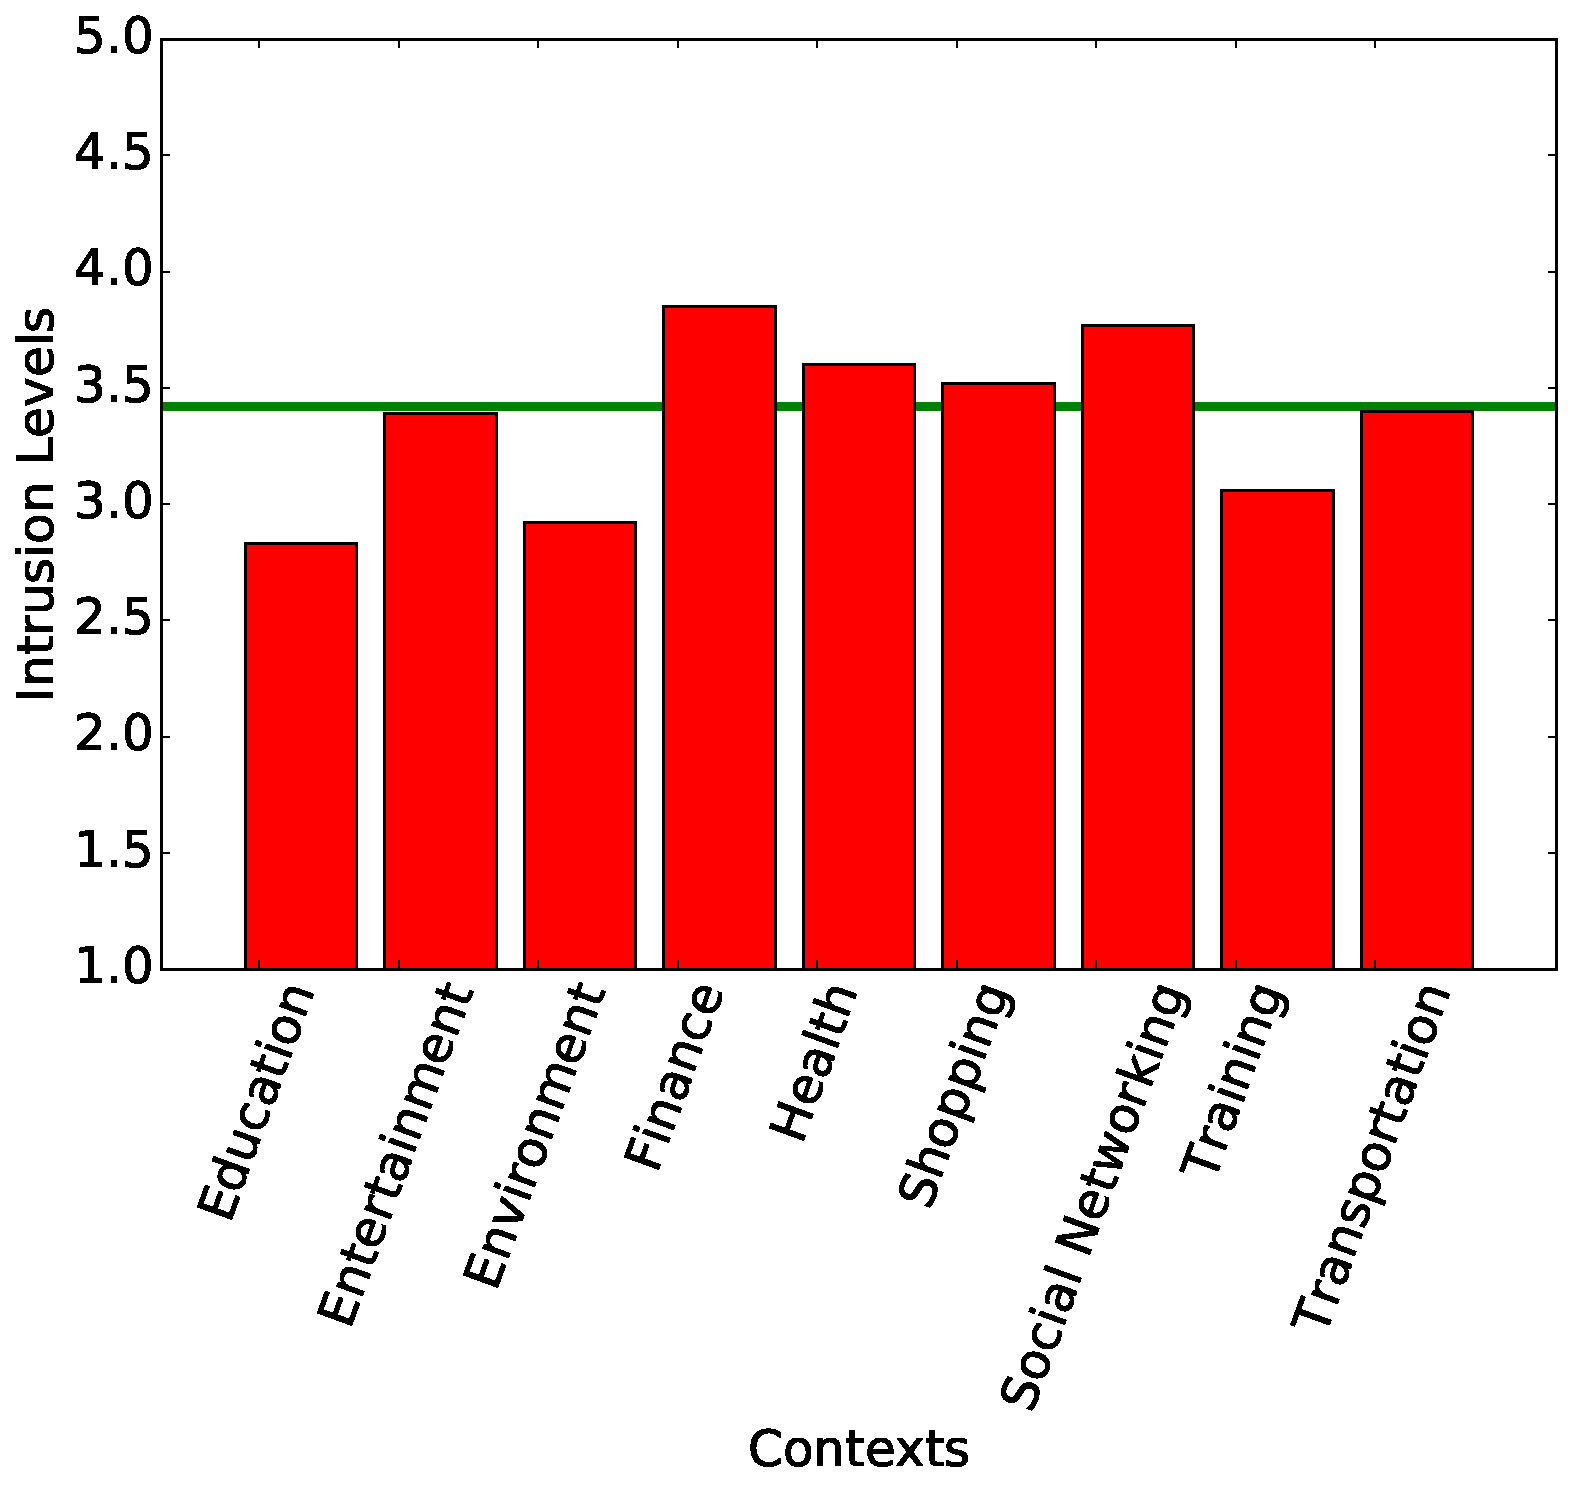
\includegraphics[width=0.5\linewidth]{./images/pre_co}}\hspace{1em}
\subtop[Standard deviation of context intrusions\label{fig:pre_13_sd}]{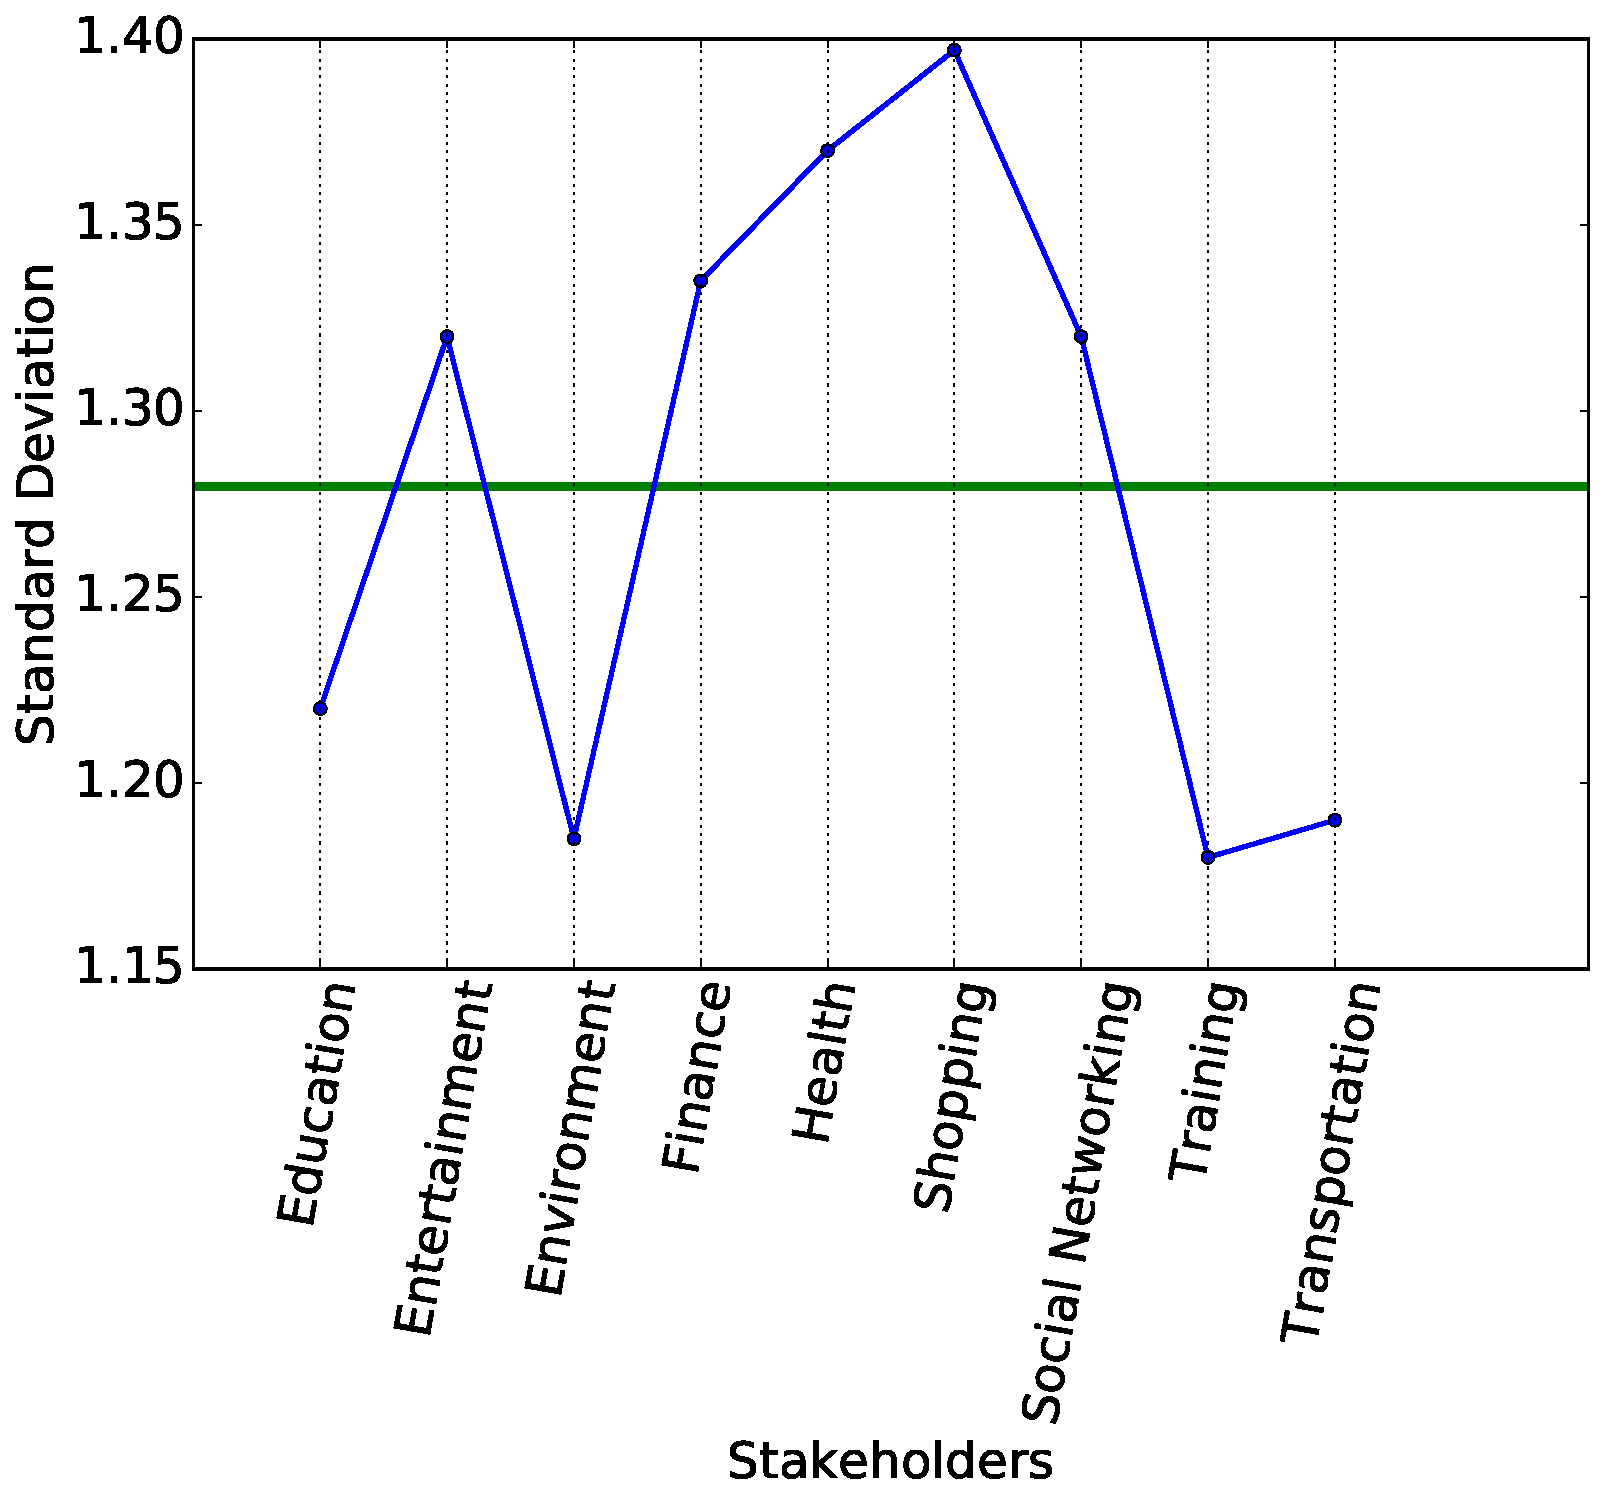
\includegraphics[width=0.5\linewidth]{./images/pre_co_sd}}\newline
\caption{Average and standard deviation for intrusion of sensors, stakeholders and contexts }
\label{fig:st3}
\end{figure}

Figure \ref{fig:pre_9} indicates the level of privacy intrusion for all sensors. Privacy intrusion level 1 corresponds to \textit{"Very low privacy intrusion"} and level 5 to \textit{"Very high privacy intrusion"}. As seen in the figure, the location, camera, microphone and bluetooth sensors are found to be most privacy intrusive with levels of 4.23, 4.14, 3.95 and 3.52 respectively. The gyroscope, battery, humidity and barometer are found to be least privacy intrusive with privacy intrusion levels of 2.13, 2.11, 2.04 and 2.00 respectively. The accelerometer, proximity, light and thermometer are found moderately intrusive with privacy intrusion levels of 2.33, 2.79, 2.31 and 2.19 respectively. Figure \ref{fig:pre_9_sd} shows the standard deviation around the mean privacy intrusion of each sensor. Among all sensors the privacy intrusion level spread around the mean is the highest for the proximity, battery, microphone, camera and bluetooth sensors.

%Among all sensors the proximity, battery, microphone, camera and bluetooth the privacy intrusion levels assigned by users has a higher spread around the mean than the rest. 
Figure \ref{fig:pre_11} indicates the level of privacy intrusion for all the stakeholders. Privacy intrusion level 1 corresponds to \textit{"Very low privacy intrusion"} and level 5 to \textit{"Very high privacy intrusion"}. As seen in the figure, the most intrusive stakeholders are corporation and government with privacy intrusion levels of 3.84 and 3.64 respectively. Stakeholders NGO and educational institution have privacy intrusion levels of 3.17 and 2.94 respectively and have privacy intrusion levels lower than the mean depicted in the figure by the horizontal line. Figure \ref{fig:pre_11_sd} shows the standard deviation around the mean privacy intrusion level for each stakeholder. As observed, stakeholder corporation and stakeholder government have a higher spread of privacy intrusion levels around the mean compared to the NGO and educational institution.

Figure \ref{fig:pre_13} indicates the level of privacy intrusion for all the contexts of applications.  Privacy intrusion level 1 corresponds to \textit{"Very low privacy intrusion"} and level 5 to \textit{"Very high privacy intrusion"}. As seen in the figure, the most privacy intrusive contexts are health, finance, shopping and social networking with levels of 3.60, 3.85, 3.50 and 3.75 respectively. The less than average privacy intrusive contexts are training, environment, entertainment, transportation and education with privacy intrusion levels of 3.06, 2.92, 3.39, 3.38 and 2.83 respectively. Figure \ref{fig:pre_13_sd} shows the standard deviation of the privacy intrusion levels for every context of application. As observed, there is a higher spread of privacy intrusion levels around the mean for contexts entertainment, finance, health, shopping and social networking.
%
%
%
%%\begin{figure}[ht!]
%%\centering
%%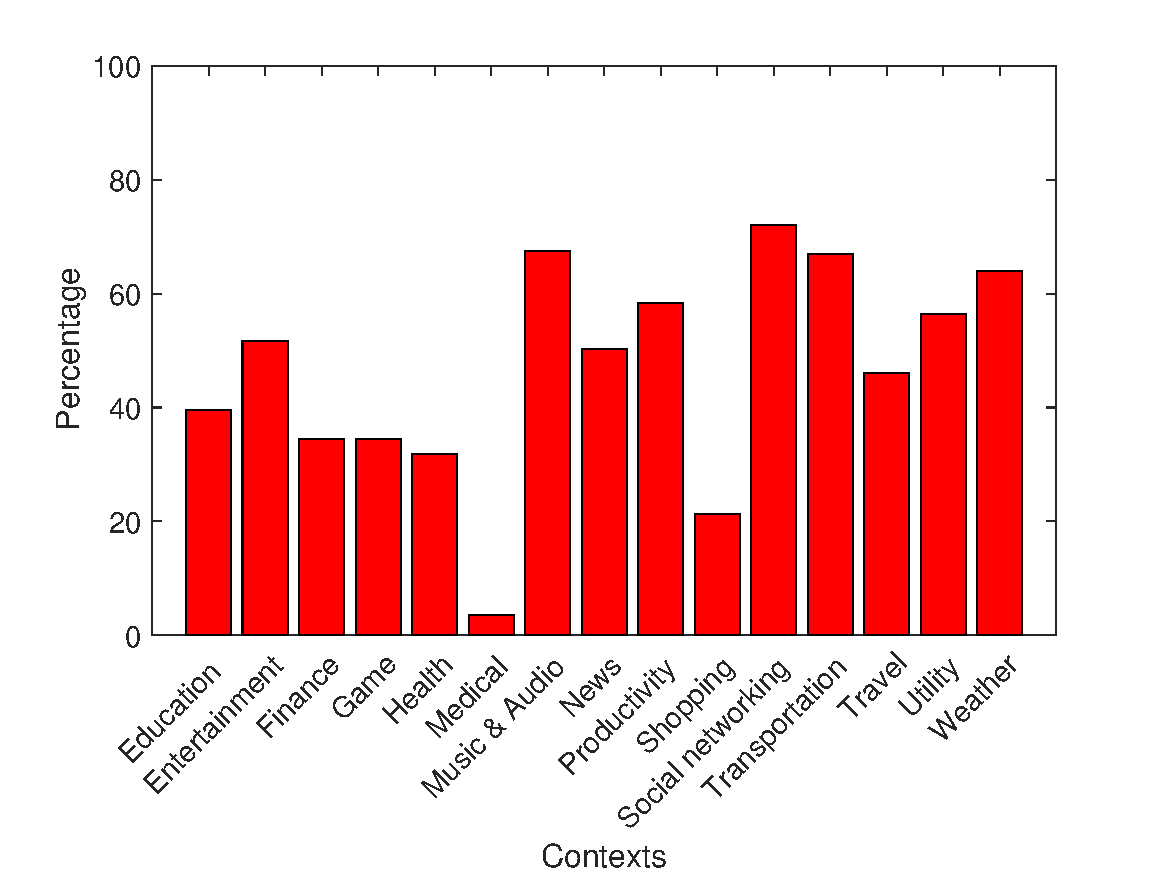
\includegraphics[width=\textwidth,keepaspectratio]{./images/pre_q6}
%%\caption{Applications in the Mobile Phone}
%%\label{fig:pre_q6}
%%\end{figure}
%%
%%\begin{figure}[ht!]
%%\centering
%%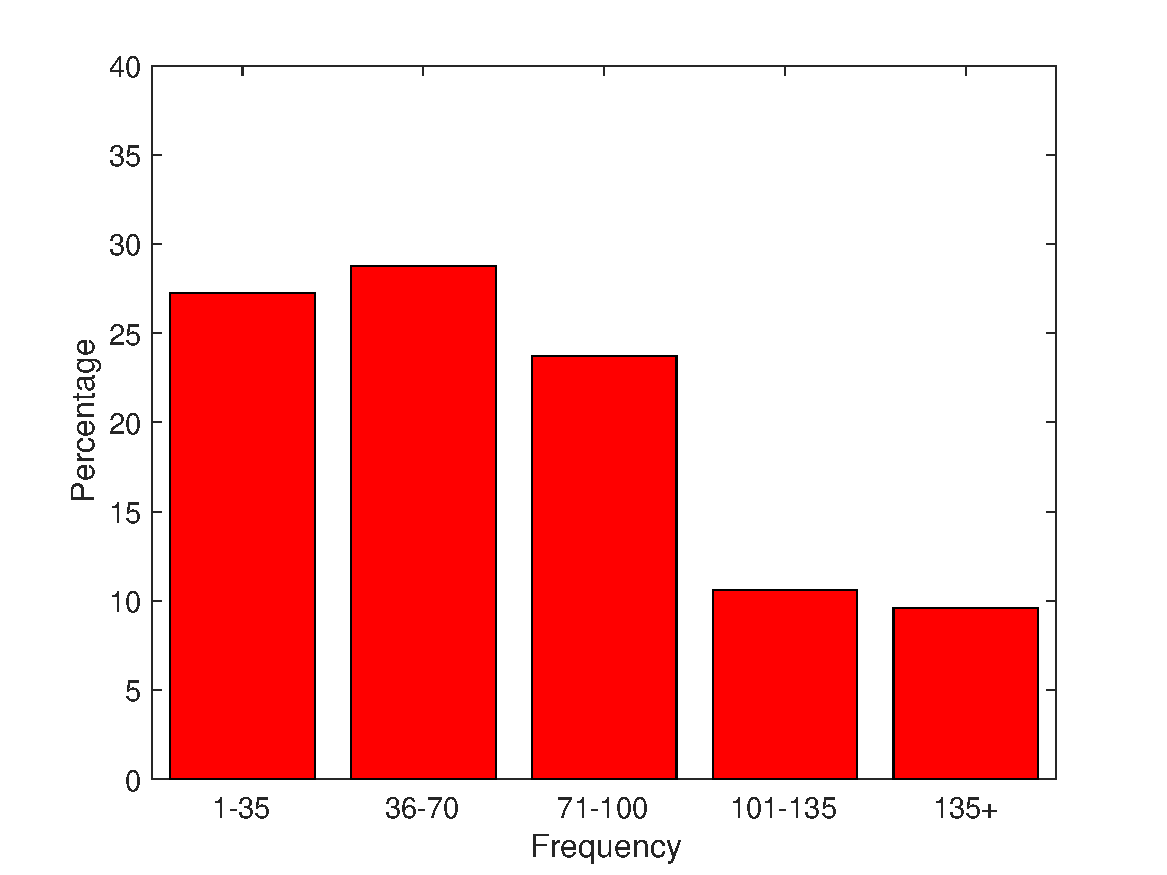
\includegraphics[width=\textwidth,keepaspectratio]{./images/pre_q7}
%%\caption{Frequency of Mobile Phone Usage}
%%\label{fig:pre_q7}
%%\end{figure}
%
%%\begin{figure}[ht!]
%%\centering
%%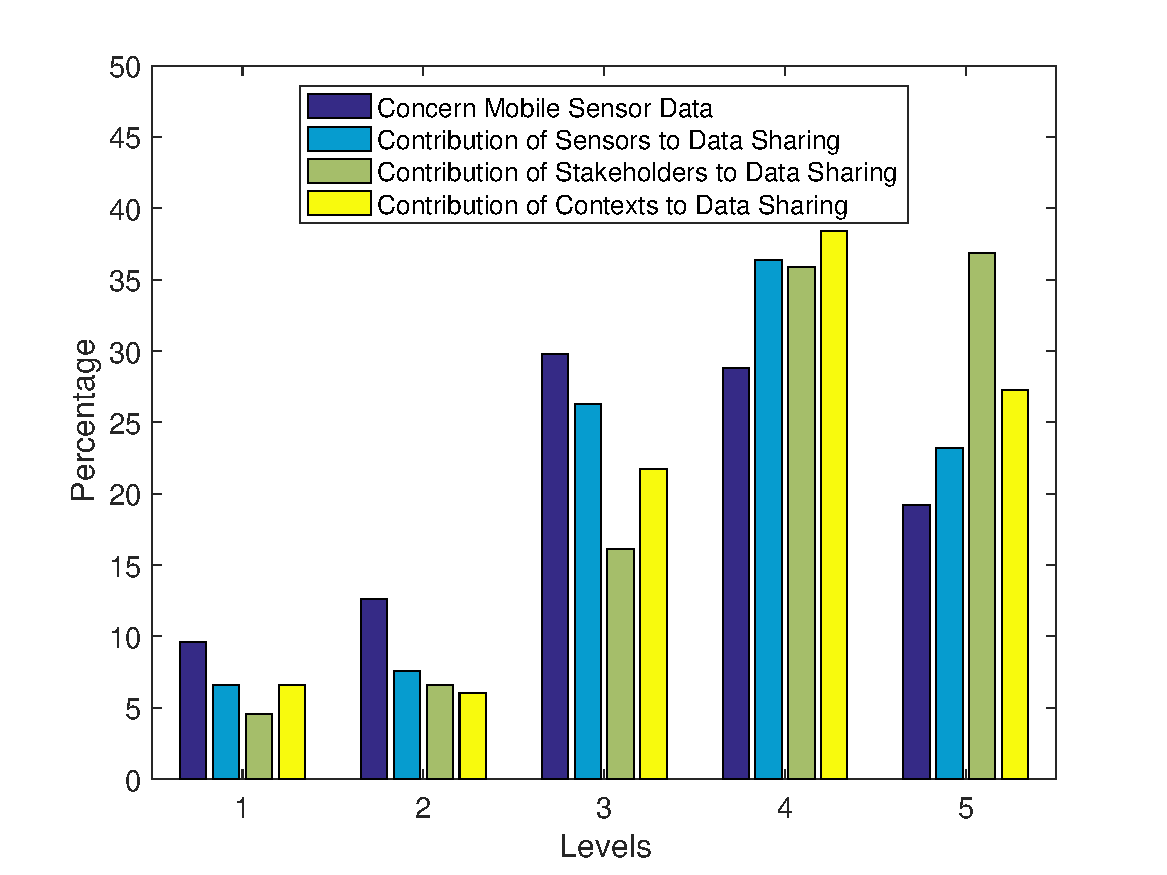
\includegraphics[width=\textwidth,keepaspectratio]{./images/pre_q8101214}
%%\caption{Graph depicting the concern of Mobile Sensor Data and the contribution of various features to the data sharing decision}
%%\label{fig:pre_q8}
%%\end{figure}
%%
%%\begin{figure}[ht!]
%%\centering
%%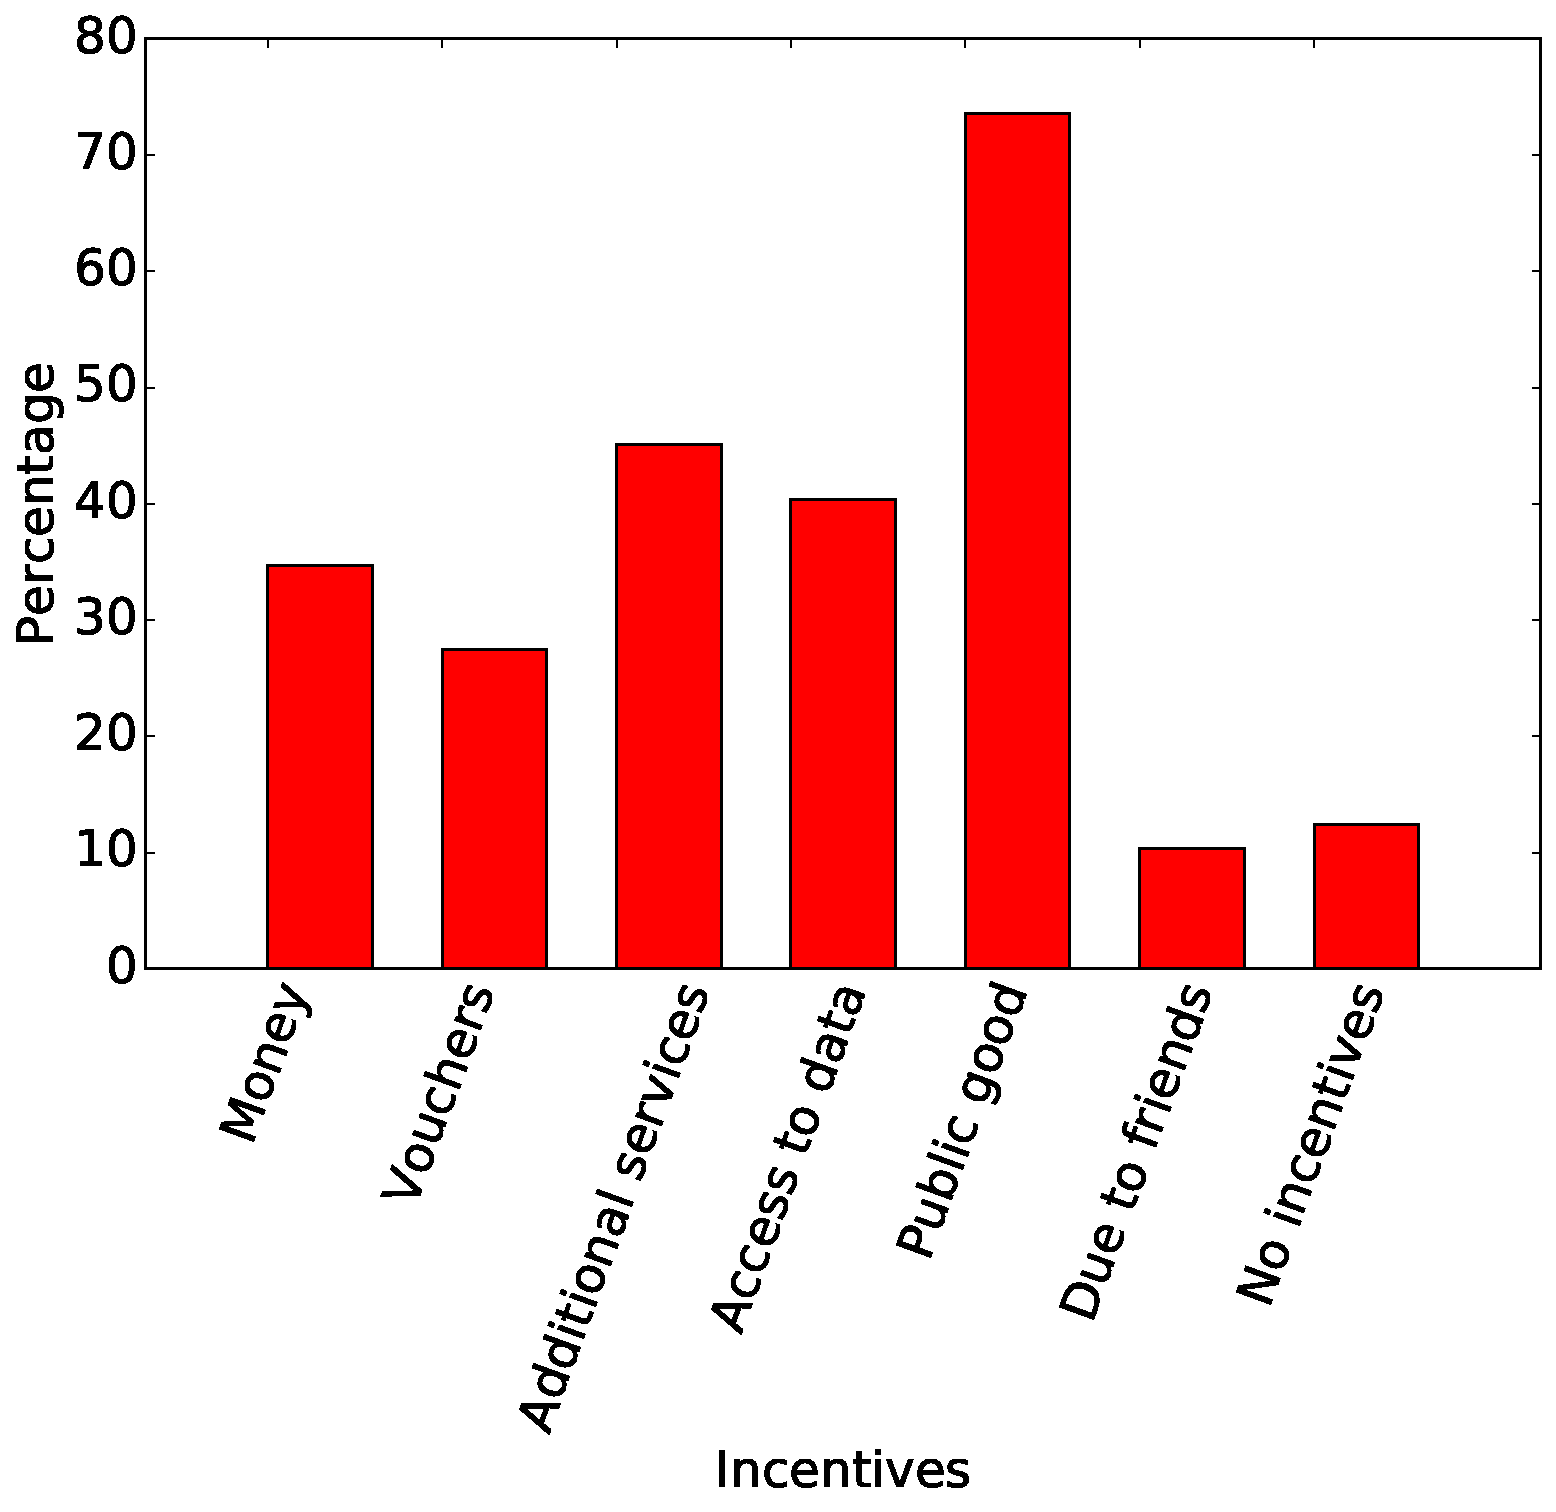
\includegraphics[width=\textwidth,keepaspectratio]{./images/pre_incentives}
%%\caption{Opinions on Incentives}
%%\label{fig:pre_q15}
%%\end{figure}
%
%
%
%%\section{Pre-Survey Methodology and Findings}
%%All the results presented below were performed on the data by performing the following changes to the data:
%%\begin{enumerate}
%%\item Rows with empty fields were removed
%%\item Rows with spurious data were removed
%%\item Data was scaled or normalized when necessary
%%\end{enumerate}
%%
%%Other than the above, the data was not manipulated. Outliers were not excluded either.
%%
%%\subsubsection{Perception of Individual Sensor Grouped on the Intrusion of Sensors in General} \label{result:sensor}
%%We try to examine here if the perception of intrusion of Sensors in general can affect the way a person views the individual sensors themselves. In other
%%words, we try to examine if there is a significant difference in perception of each sensor depending on the perception of the Sensors as a whole.
%%For this, we grouped the survey data based on the responses to question 10, which examines the contribution of sensors in general for a data request. Since there are 5 possible responses to this question, this makes 5 individual groups from 1 to 5.
%%
%%The reason why this is necessary is because, if users who view Sensors in general view in the same manner all the individual sensor sub-features, there would be no need to ask users to individually categorize each sub-feature, a profile can be formed just based on feature categorizations.
%%
%%Five groups of users are formed from one to five, who view Sensors as a whole with different intrusion levels and their perception of each of the individual sensors is now to be compared. Before going into the comparison, we try to understand the properties of the data to analyze. Essentially, we try to examine if each of the groups formed come different populations and for this the most popular statistical tests is the one-way ANOVA. To perform a one-way ANOVA test, the data should be\footnote{\url{https://fr.wikipedia.org/wiki/Analyse\_de\_la\_variance}}:
%%
%%\begin{enumerate}
%%\item Normally distributed
%%\item Homoscedastic
%%\item Ordinal or continuous
%%\end{enumerate}
%%
%%Since the data of the survey is discrete and follows the Likert Scale with options from 1 to 5, it gives a skewed normal distribution. The scale used to collect data is in the ordinal form. Additionally, the variances of values within the groups formed are not similar. The one-way ANOVA test is quite robust to heteroscedacity, as long as the maximum variance among all groups is less than four times the group with the lowest variance.  Accounting for all the violations, we instead opt for non-parametric tests such as the Kruskal-Wallis H-test and the Dunn's test
%%which only assumes the following\footnote{\url{https://en.wikipedia.org/wiki/Kruskal-Wallis\_one-way\_analysis\_of\_variance}} : 
%%
%%\begin{enumerate}
%%\item Groups are independant from one another
%%\item All observations are independant
%%\item The dependant variables should be in the ordinal scale or continuous
%%\end{enumerate}
%%
%%The above tests do not make any assumptions about the distribution of the data and are robust to heteroscedastic data.
%%\begin{figure}[htp]
%%\subtop[Mean of each Group for each Sensor\label{fig:s1}]{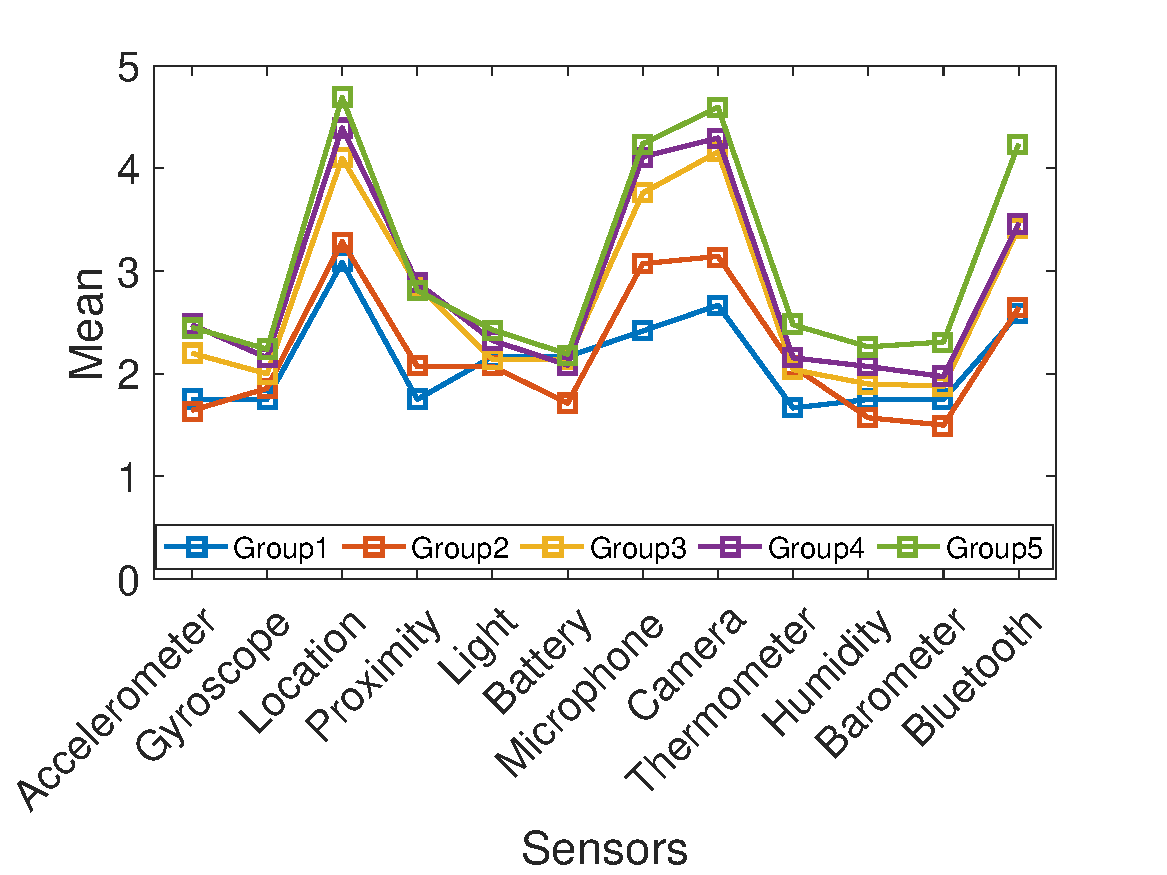
\includegraphics[width=0.5\linewidth,height=0.45\linewidth]{./images/sensors_group_meanQ10}}
%%\subtop[Variance of each Group for each Sensor\label{fig:s2}]{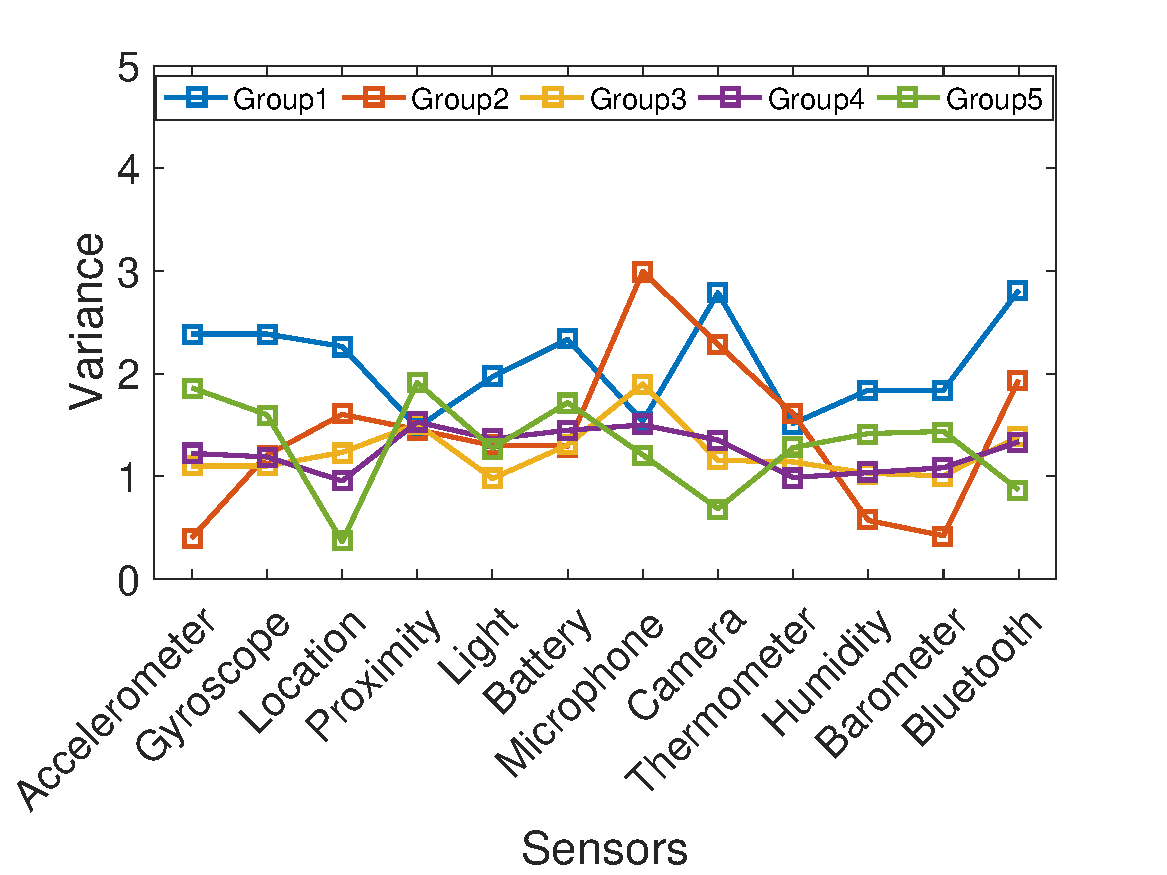
\includegraphics[width=0.5\linewidth,height=0.45\linewidth]{./images/sensors_group_varianceQ10}}
%%\caption{Table Schemas}
%%\label{fig:s3}
%%\end{figure}
%%
%%Group 1 to 5 which consist of users with different perception of Sensors have 13, 14, 50, 71 and 42 people in each group respectively. For in depth information of the composition of each group in terms of employment, education, gender and birth year please refer to tables
%%\ref{tab:emp_sensors}, \ref{tab:edu_sensors}, \ref{tab:gender_sensors}, \ref{tab:year_sensors}. Figures \ref{fig:s1} and \ref{fig:s2} depict the mean and variances for each of the individual groups. 
%%
%%We start by performing the non paramteric Kruskal-Wallis test for each individual sensor. The value of alpha assumed here is 0.05. The null hypothesis states that all the groups perceive all the sensors in the similar way. This means they come from the same population. The alternative hypothesis is
%%that the groups perceive each sensor in a significantly different way and hence their populations are distinct. The table \ref{tab:kw_sensors} depicts the p-values obtained from the statistical test.
%%
%%\begin{table}[h!]
%%  \centering
%%  \caption{Kuskal-Wallis Test For Sensors}
%%  \label{tab:kw_sensors}
%%  \begin{tabular}{cccc}
%%    \toprule
%%     Sensor & p-value \\
%%    \midrule
%%    Accelerometer & 0.0151 \\
%%    Gyroscope & 0.2959\\
%%    Location & 1.0664e-05\\
%%    Proximity & 0.0147\\ 
%%    Light & 0.6933\\
%%    Battery & 0.6950\\ 
%%    Microphone & 3.0070e-04\\
%%    Camera & 2.1191e-05\\
%%    Thermometer & 0.0693\\ 
%%    Air Humidity & 0.1292\\
%%    Barometer & 0.0949\\
%%    Bluetooth & 3.4877e-05\\ 
%%    \bottomrule
%%  \end{tabular}
%%\end{table} 
%%
%%Accelerometer, location, proximity, microphone, camera and bluetooth are the sensors for which the group opinions vary significantly.
%%On these sensors, we proceed with a post hoc test for further investigation by performing a pariwise Dunn's test to examine if there is an actual significant difference between the groups and if so between which groups. The sensors with p-values with less than 0.05 are examined in more detail and the p-values are presented in table \ref{tab:dunn_sensors}. The table shows the results for each pairwise test done, with the p-values adjusted using the Bonferroni Method\footnote{\url{https://en.wikipedia.org/wiki/Bonferroni\_correction}}. The reason for choosing to adjust the p-values is that repeated experiments can increase the chances of accepting the alternative hypothesis so p-values are adjusted according to the number of experiments performed. 10 experiments are performed per sensor.
%%
%%For the accelerometer and proximity sensors, it is seen that none of the pairwise groups have a significant difference from each other. This means that even tough the groups perceive sensors differently in general, they all view accelerometers and proximity sensors in a similar way. This is reinforced by figures \ref{fig:se_acc} and \ref{fig:se_prox}, where it is seen that there is significant overlap between the population of the groups.
%%
%%For the location sensor, it is observed that groups (1,4), (1,5), (2,4), (2,5) have a significant difference. This can be attributed to the fact that since the groups are formed from the perception of people of the sensors feature, the difference in perception between group 1 and group 5 will be larger than between group 1, group 2 and group 1, group 3 since they are not much apart in the scale. Figure \ref{fig:se_loc} depicts the spread of the group populations for the location sensor. As found groups (1,4), (1,5), (2,4), (2,5) have the least amount of overlap.
%%
%%For the microphone sensor, it can be seen that groups (1,3), (1,4) and (1,5) are significantly different from each other. This goes to show that
%%if people rate sensors as even a little intrusive, they all rate the microphone's in a significantly different way than the people who rate sensors as non-intrusive. Figure \ref{fig:se_micro} depicts the spread of the population of the groups.
%%
%%For the camera sensor, it can be observed that groups (1,4), (1,5), (2,4), (2,5) have a significant difference in their perception of the intrusion. Similar to the location sensor, people with perception of sensors in general with a lower intrusion level have significantly different responses to the camera intrusion than the people who rate sensors with more intrusion. Figure \ref{fig:se_cam} depicts the spread of the population of the groups for the camera sensor.
%%
%%For the Bluetooth sensor, there is a significant difference between groups (1,5), (2,5), (3,5) and (4,5). This shows that responses by people who find sensors extremely intrusive is different from the rest of the groups. This fact is reinforced by figure \ref{fig:se_blue} where it is seen that group 5 has least overlap with other groups.
%%
%%It can be concluded that some sensors such as the accelerometer, proximity, gyroscope, light, battery, thermometer, humidity, barometer are sensors where each of the groups do not have significantly different opinions of intrusion. Sensors such as the camera, microphone, location and bluetooth
%%are where opinions differ between groups. These sensors are found to be on average more intrusive with intrusion values of 4.23, 3.87, 4.14 and 3.52 respectively on a scale of five. Groups with larger differences between them (such as groups 1 and 4) tend to have larger differences in opinions for some sensors generally considered intrusive. Groups with smaller differences between them (such as group 1 and 2) tend to have similar opinions.
%%
%%Even tough users tend to see sensors as a whole in a different light, all groups can be incentivized similarly for lower intrusion sensors. For higher intrusion sensors, groups need to be incentivized differently, with higher intrusion groups receiving more incentives.
%%
%%\begin{table}[h!]
%%  \centering
%%  \caption{Dunn's Test For Sensors}
%%  \label{tab:dunn_sensors}
%%  \begin{tabular}{ccccccc}
%%    \toprule
%%     Groups & Accelerometer & Location & Proximity & Microphone & Camera & Bluetooh \\
%%    \midrule
%%    (1,2) & 1.0000 & 1.0000 & 0.9992 & 0.8365 & 1.0000 & 1.0000 \\
%%    (1,3) & 0.4207 & 0.2084 & 0.0699 & 0.0365 & 0.0732 & 0.7825 \\
%%    (1,4) & 0.0595 & 0.0125 & 0.0513 & 0.0012 & 0.0048 & 0.6442 \\
%%    (1,5) & 0.2054 & 0.0010 & 0.1191 & 0.0009 & 0.0007 & 0.0029 \\
%%    (2,3) & 0.6548 & 0.1774 & 0.3713 & 0.8927 & 0.1694 & 0.5921 \\
%%    (2,4) & 0.1185 & 0.0077 & 0.2617 & 0.2287 & 0.0123 & 0.4270 \\
%%    (2,5) & 0.3659 & 0.0005 & 0.5184 & 0.1597 & 0.0018 & 0.0007 \\
%%    (3,4) & 0.8989 & 0.7642 & 1.0000 & 0.8052 & 0.9040 & 1.0000 \\
%%    (3,5) & 0.9997 & 0.0869 & 1.0000 & 0.6390 & 0.2947 & 0.0066 \\
%%    (4,5) & 0.9998 & 0.8360 & 1.0000 & 1.0000 & 0.9617 & 0.0059 \\
%%    \bottomrule
%%  \end{tabular}
%%\end{table} 
%%
%%\begin{figure}[htp]
%%\subtop[Accelerometer\label{fig:se_acc}]{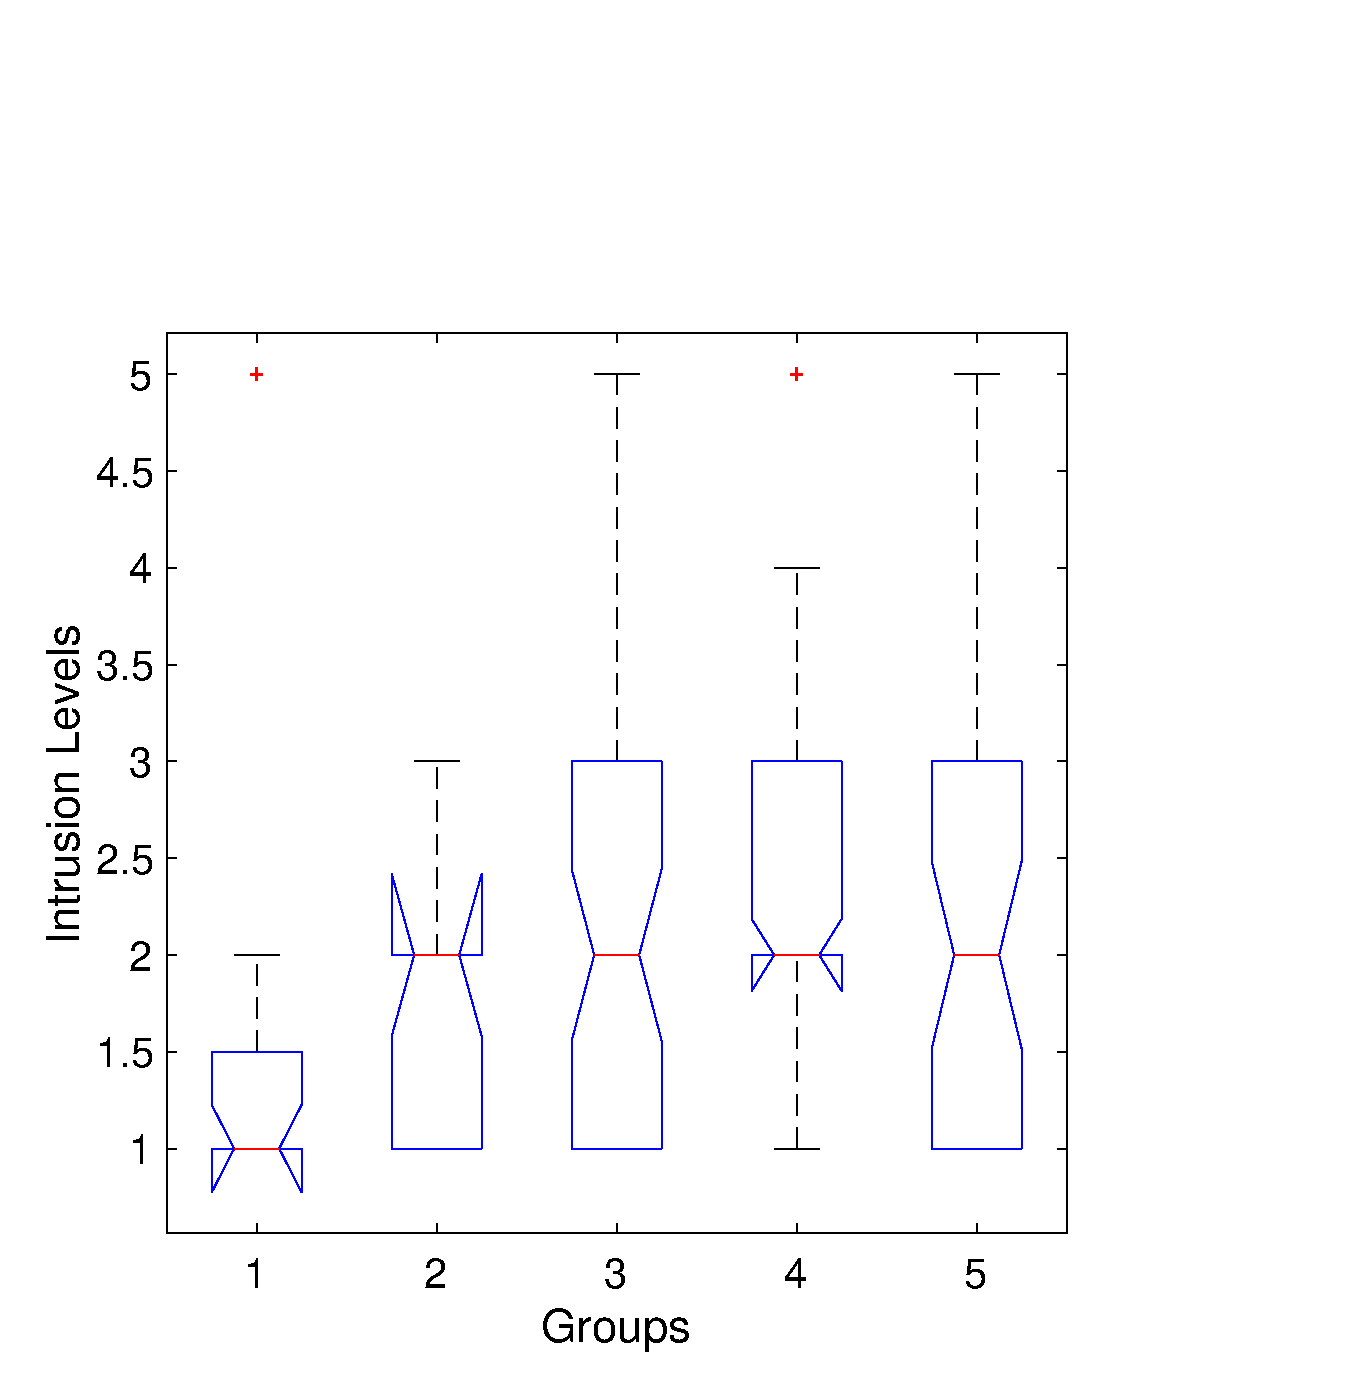
\includegraphics[width=0.5\linewidth]{./images/acc_box}}\hspace{1em}
%%\subtop[Location\label{fig:se_loc}]{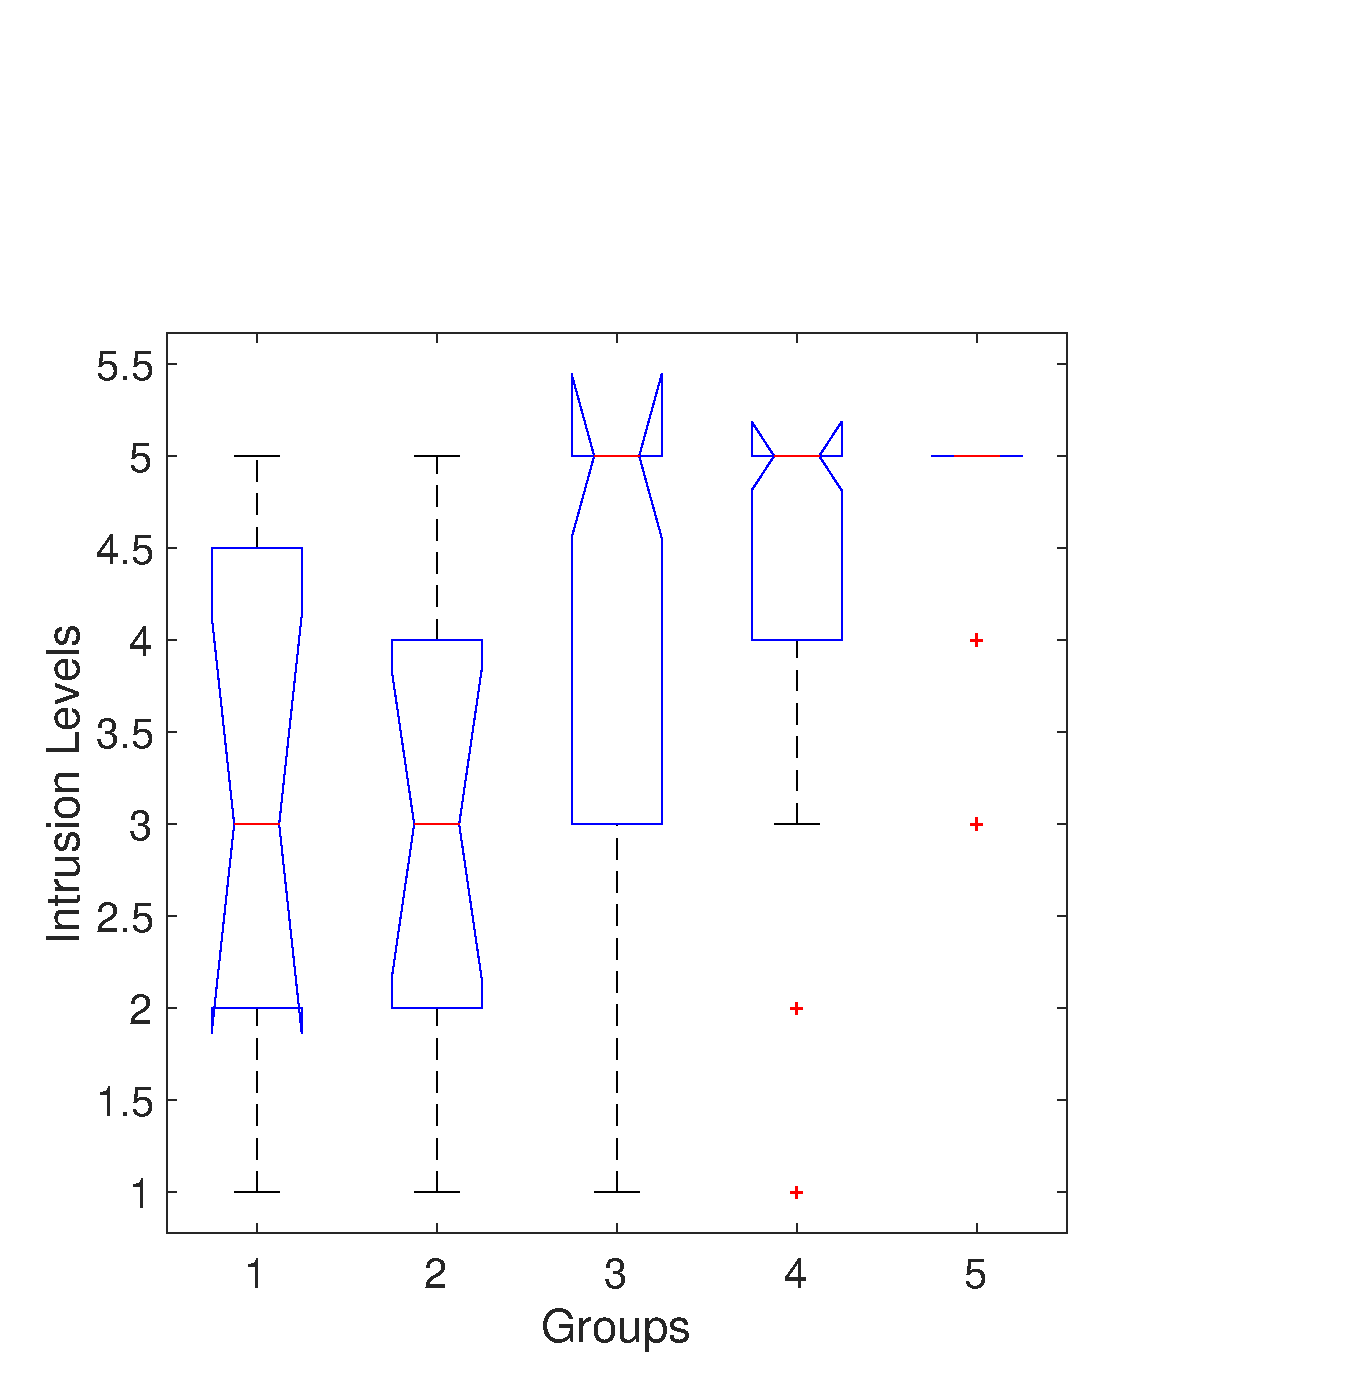
\includegraphics[width=0.5\linewidth]{./images/loc_box}} \newline
%%\subtop[Proximity\label{fig:se_prox}]{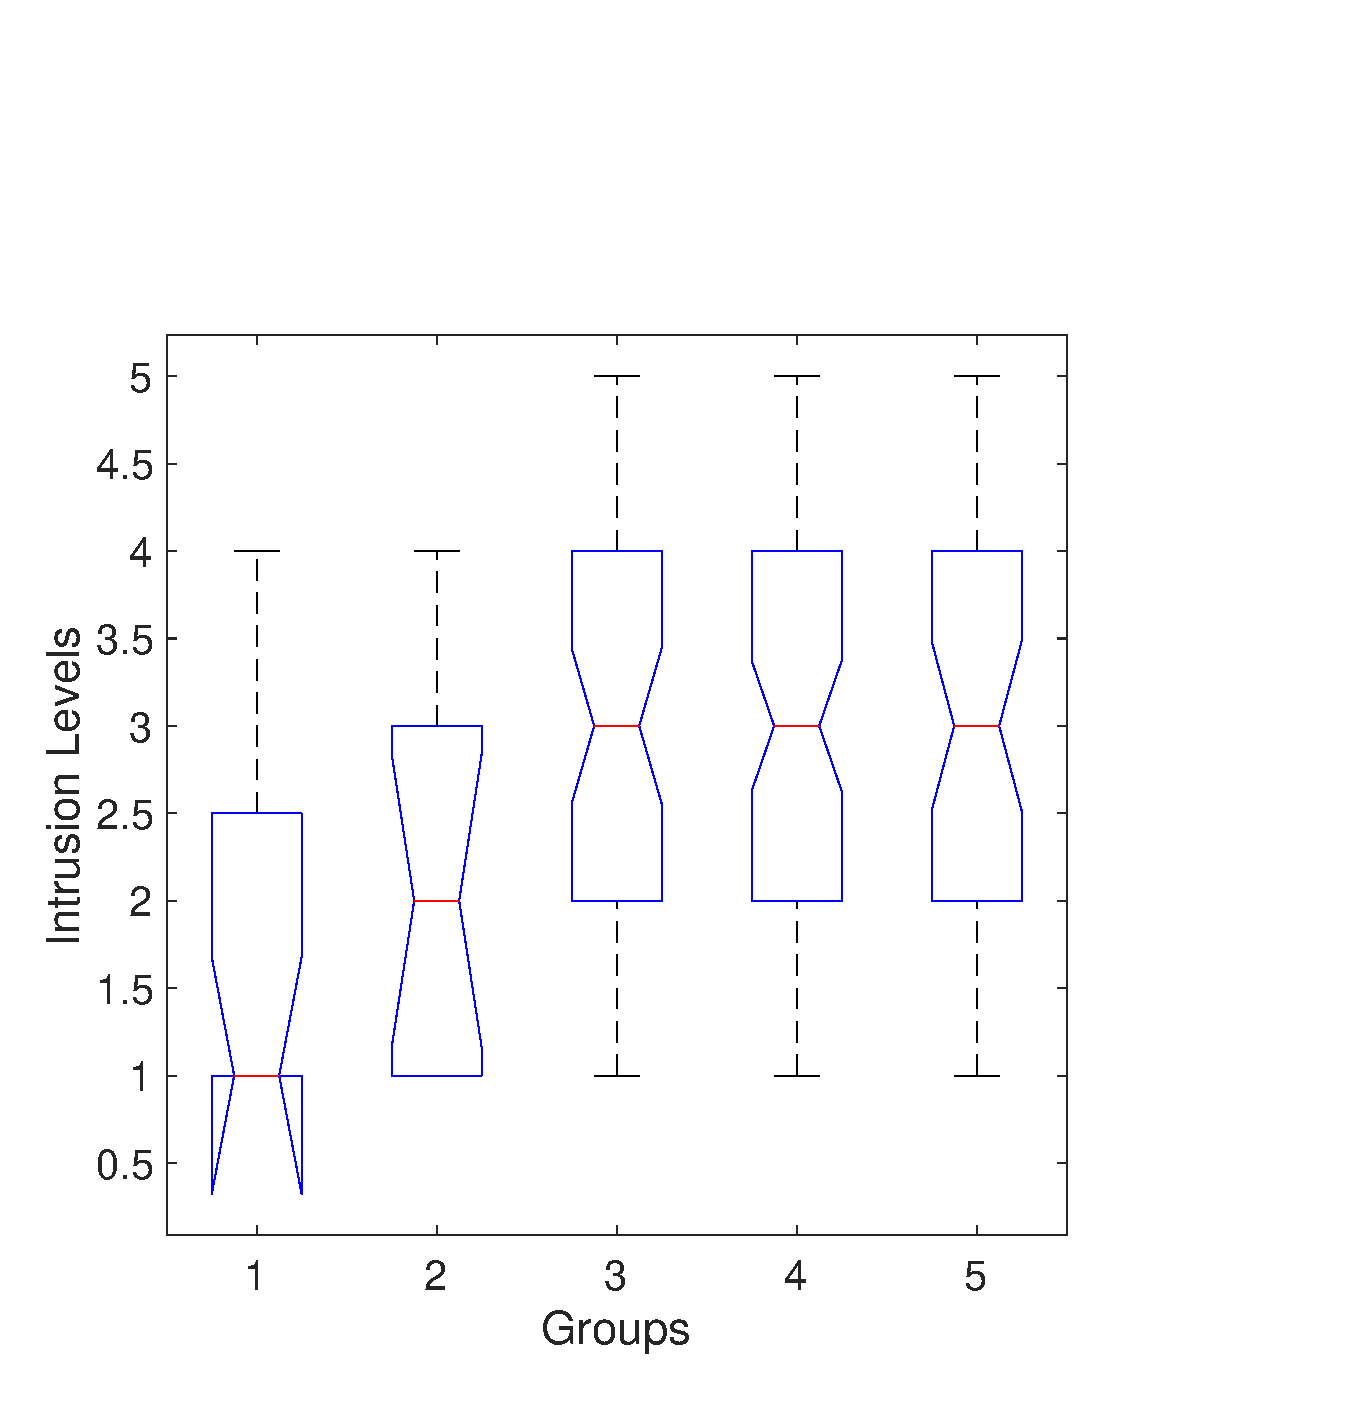
\includegraphics[width=0.5\linewidth]{./images/prox_box}}\hspace{1em}
%%\subtop[Microphone\label{fig:se_micro}]{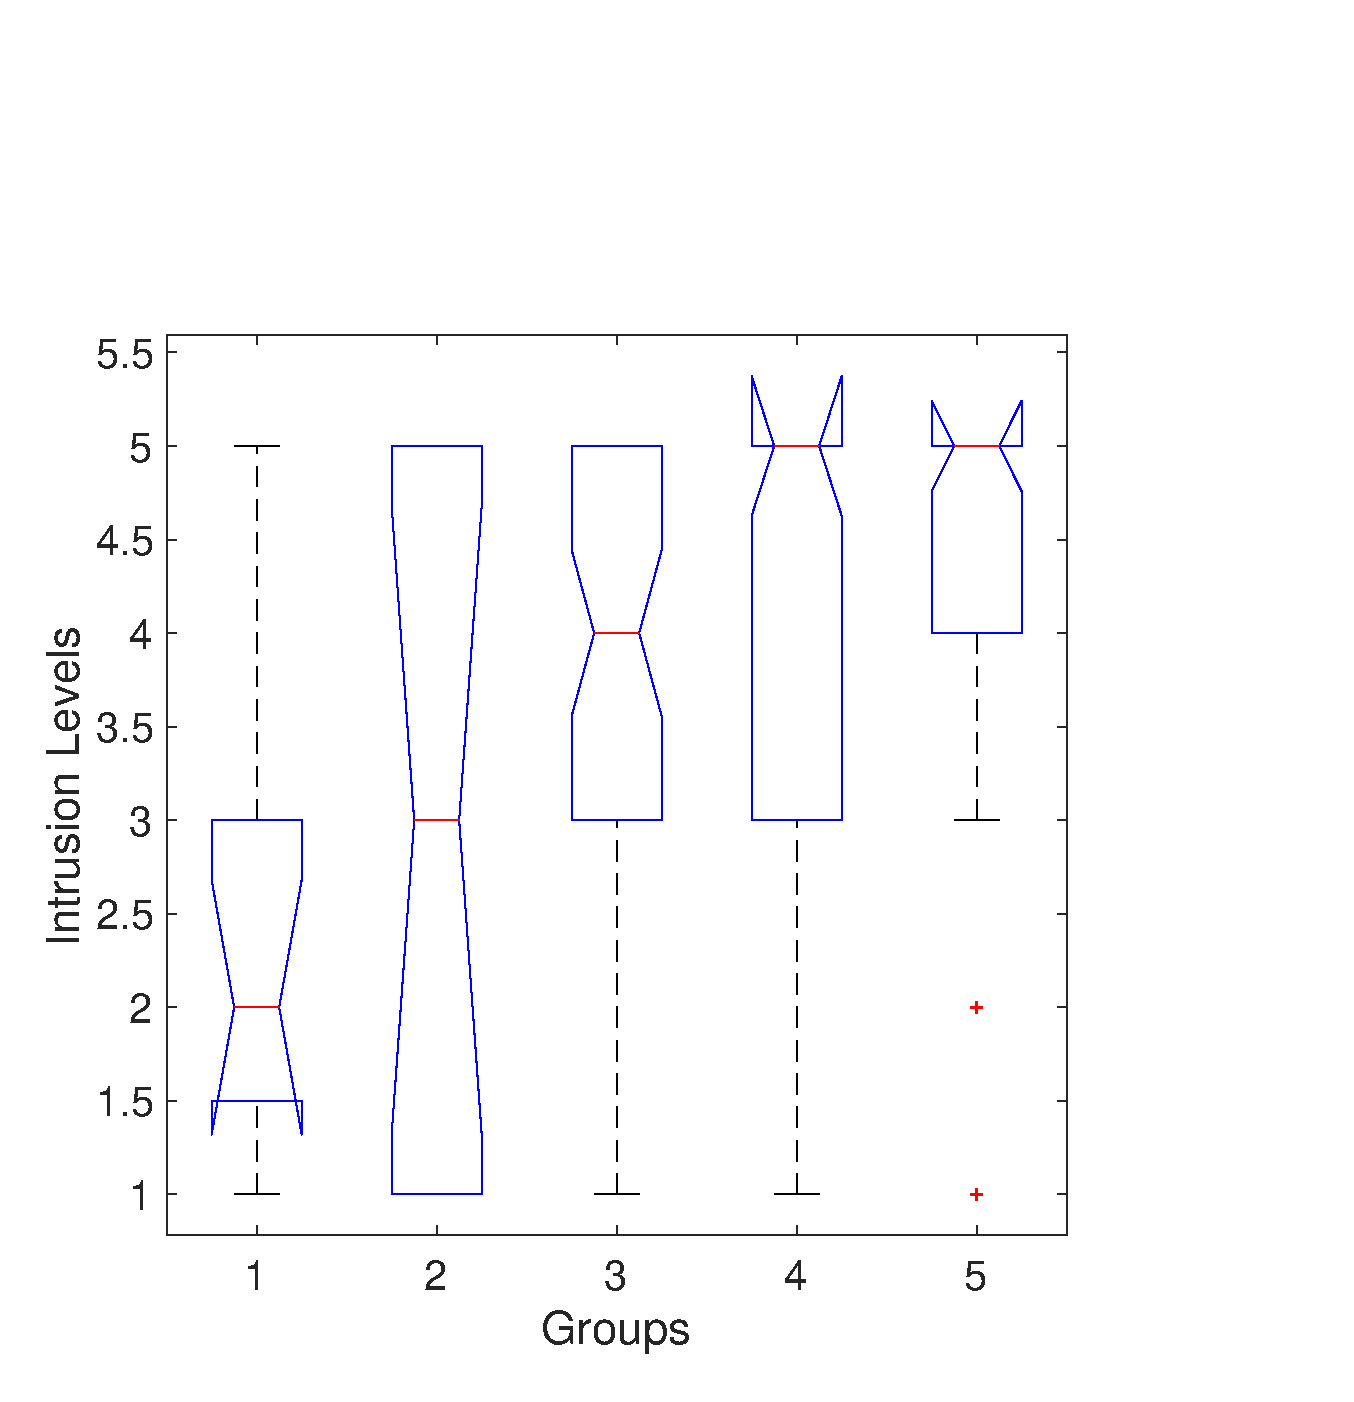
\includegraphics[width=0.5\linewidth]{./images/micro_box}} \newline
%%\subtop[Camera\label{fig:se_cam}]{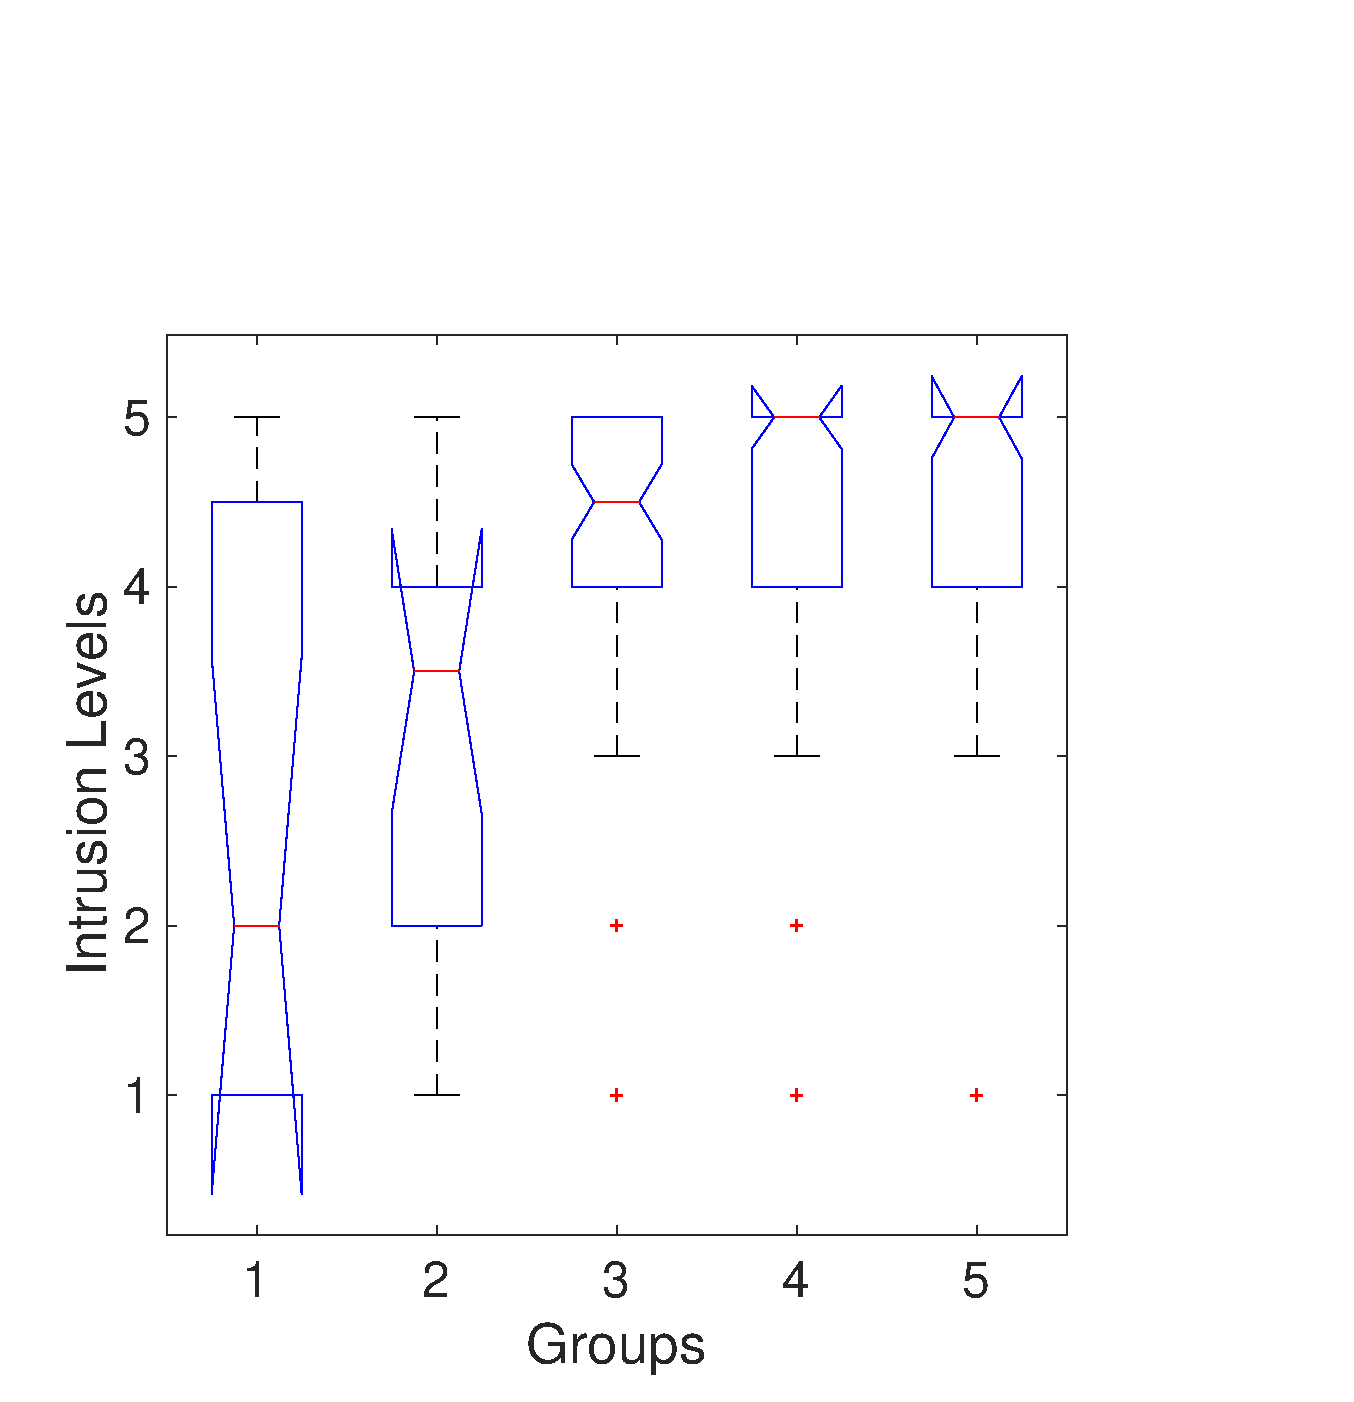
\includegraphics[width=0.5\linewidth]{./images/camera_box}}\hspace{1em}
%%\subtop[Bluetooth\label{fig:se_blue}]{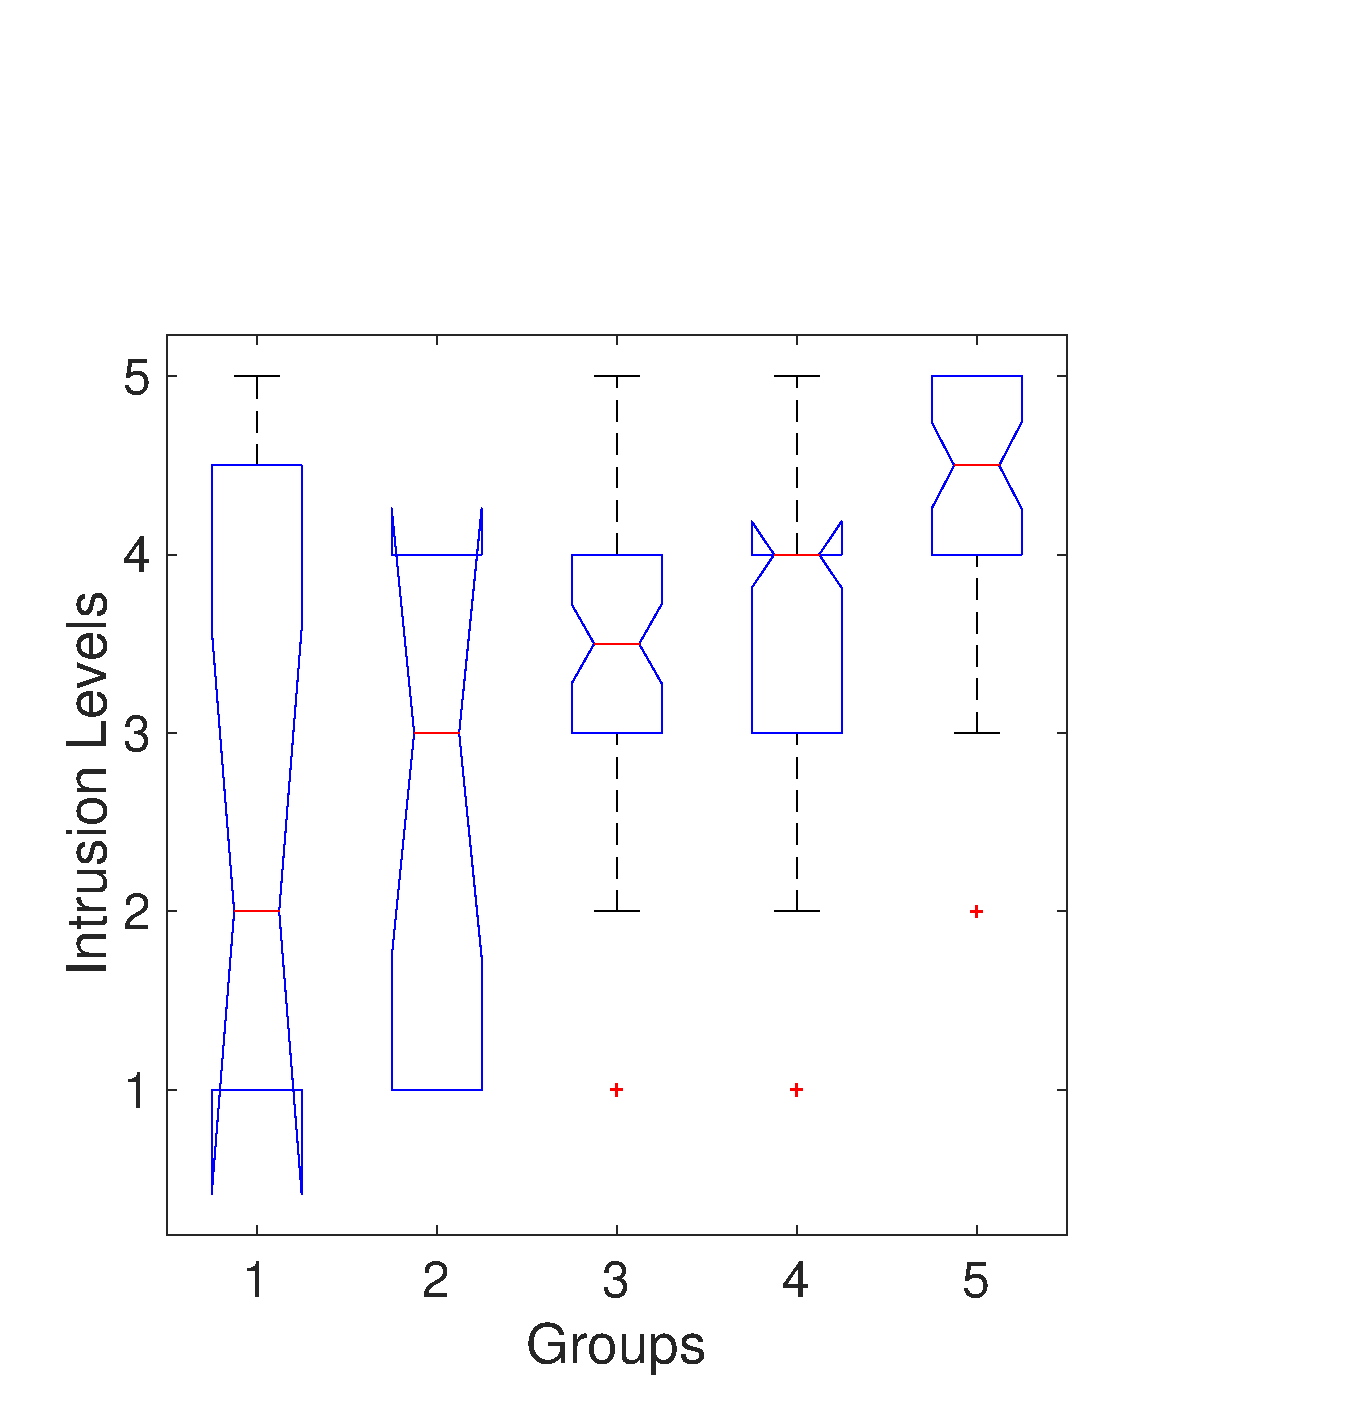
\includegraphics[width=0.5\linewidth]{./images/blue_box}}
%%\caption{Box Plots Indicating the Population Spread of each Group}
%%\label{fig:st3}
%%\end{figure}
%%
%%
%%\subsubsection{Perception of Individual Stakeholders Grouped on the Intrusion of Stakeholders in General}
%%
%%In this section, we try to see if the intrusion level perception by people of Stakeholders in general is linked to the intrusion of the individual stakeholders. In other words we examine the significant differences between groups formed by using question 12's responses (which looks into the perception of users for stakeholders in general) on the perception of
%%each individual stakeholder. Since there are 5 different responses to question 12 ,this results in five independent groups. The groups 1 to 5 have 7, 11, 32, 69 and 70 people in each group respectively. More detailed information about the employment, education, gender and age distribution in the groups is given in tables \ref{tab:emp_stak}, \ref{tab:edu_stak}, \ref{tab:gender_stak} and \ref{tab:year_stak}. The mean and variances of each group formed is depicted in figures \ref{fig:st1} and \ref{fig:st2}.
%%
%%\begin{figure}[htp]
%%\subtop[Mean of each Group for each Stakeholder\label{fig:st1}]{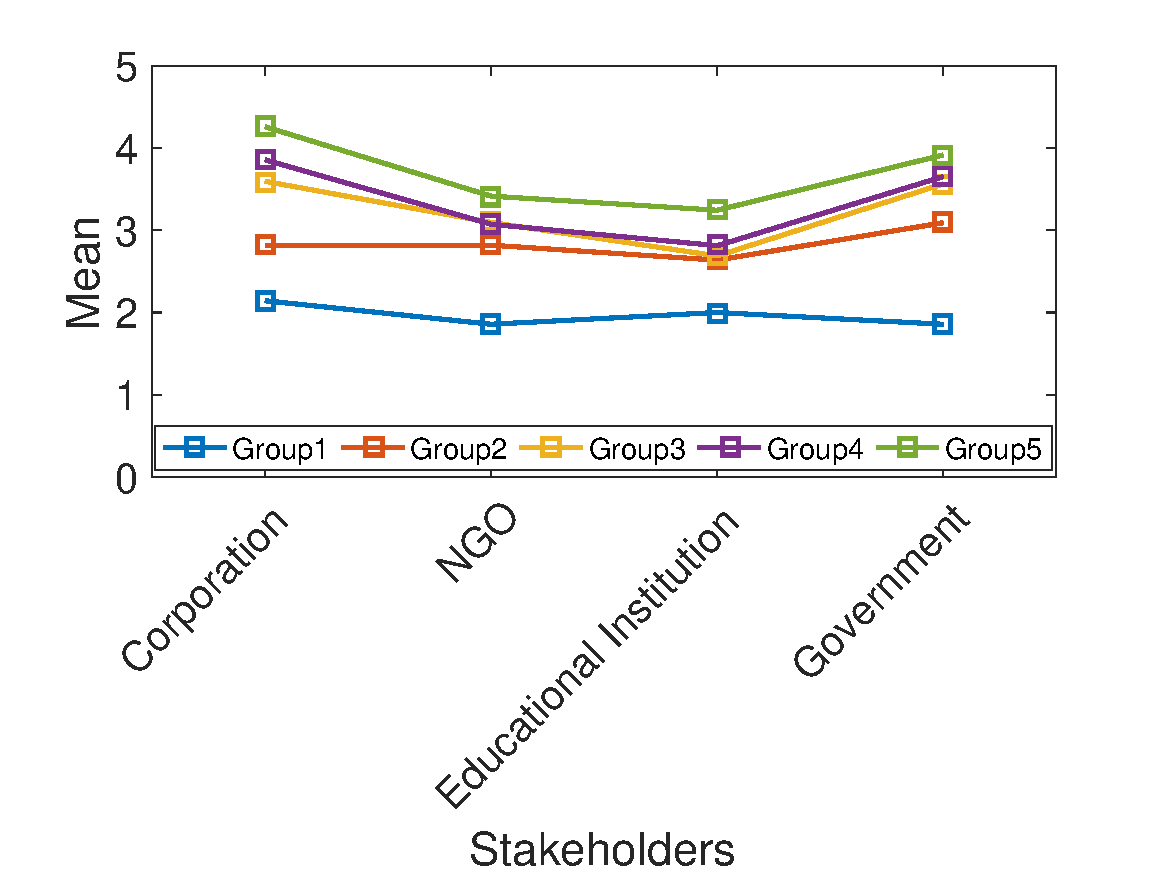
\includegraphics[width=0.5\linewidth,height=0.45\linewidth]{./images/stakeholders_group_meanQ12}}
%%\subtop[Variance of each Group for each Stakeholder\label{fig:st2}]{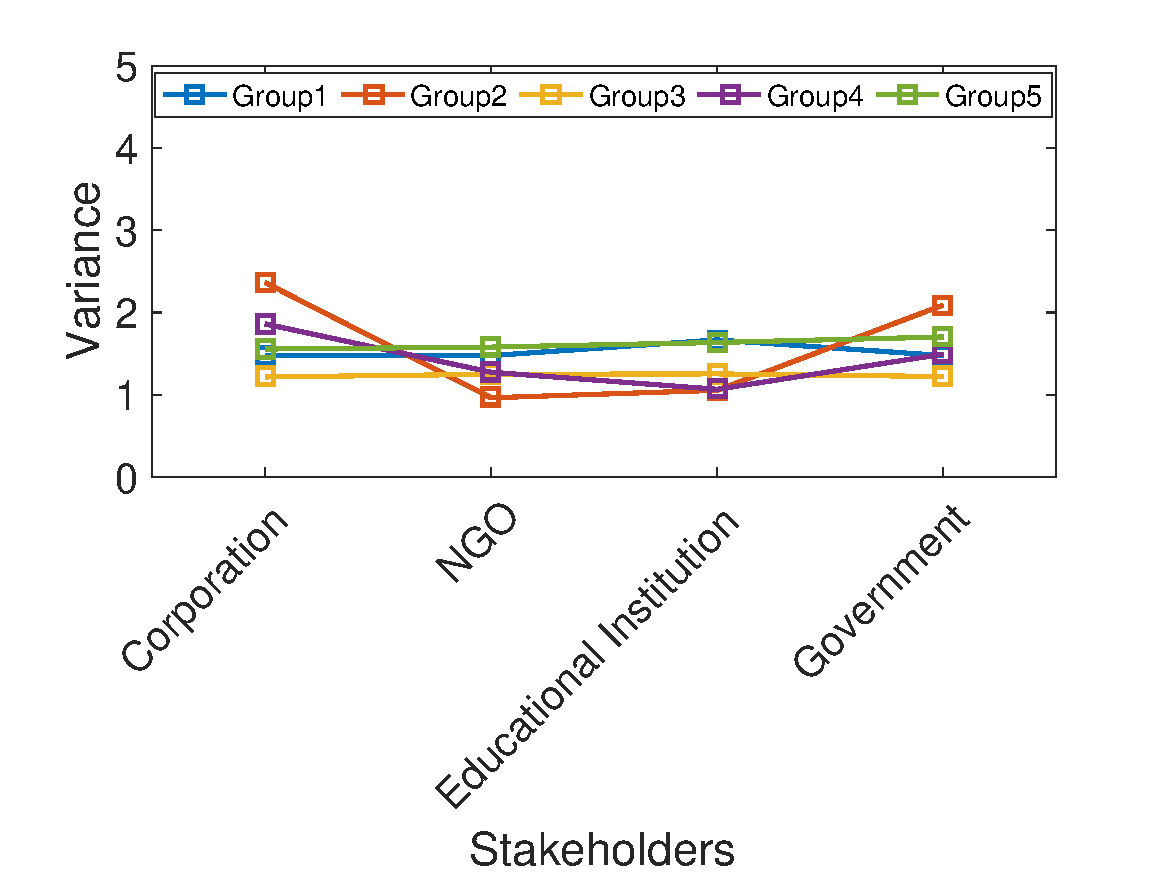
\includegraphics[width=0.5\linewidth,height=0.45\linewidth]{./images/stakeholders_group_varianceQ12}}
%%\caption{Mean and Variance of Groups}
%%\label{fig:st3}
%%\end{figure}
%%
%%To start, we examine all the groups simultaneously for all the individual stakeholders. The Kruskal-Wallis H-test since the data is discrete and not normally distributed. Further detail about the reason the test is chosen is provided in the previous section \ref{result:sensor}. The null hypothesis states that all the groups rate the intrusion of each stakeholder in a similar way. The alternative hypothesis is that the groups rate the intrusion of each stakeholder in a significantly different way.
%%
%%The resulting p-values of this test are displayed in table \ref{tab:kw_stak}. As it is seen, the test pronounces that all the groups are significantly different at an alpha with 0.05 for all stakeholders. 
%%
%%
%%\begin{table}[h!]
%%  \centering
%%  \caption{Kuskal-Wallis Test for Stakeholders}
%%  \label{tab:kw_stak}
%%  \begin{tabular}{cc}
%%    \toprule
%%     Stakeholder & p-value \\
%%    \midrule
%%    Corporation & 2.1432e-05 \\
%%    Non-Governmental Organization & 0.0221\\
%%    Educational Institution & 0.0396\\
%%    Government & 0.0024\\ 
%%    \bottomrule
%%  \end{tabular}
%%\end{table}
%%
%%This prompts us to take a closer look at which of the groups are significantly different from each other for each stakeholder. For this, we continue the experiment by performing a Dunn's Test with p-values adjusted by the Bonferroni Method. The results from the tests are shown in table \ref{tab:dunn_stak}. The test was done for all stakeholders since the Kruskal-Wallis test denoted that all groups differ significantly for all stakeholders. 
%%
%%Looking at the stakeholder corporation, it is seen that groups (1,4), (1,5) and (2,5) differ significantly. This goes to show that groups with larger differences in their outlook to stakeholders as a whole view corporations in a significantly different way. Figure \ref{fig:st_corp} shows the spread of each group for corporations. It is observed that adjacent groups have a large overlap.
%%
%%For the non-governmental organizations, only the groups (1,5) differ significantly. This goes to show that groups that do not find stakeholders intrusive and groups that find stakeholders very intrusive rate the intrusion of Non-Governmental Organization in significantly different ways. Additionally, it shows that groups with large differences in the perception of stakeholders have significant differences in their perceptions on NGOs. Figure \ref{fig:st_ngo} reinforces this claim.
%%
%%For Educational Institutions, none of pairwise comparisons have p-values below 0.05. This goes to show that the intrusion of Educational Institutions by all groups does not differ significantly, that is all groups have similar opinions. Figure \ref{fig:st_edu} shows that all groups have significant overlap.
%%
%%Lastly, for the stakeholder government, the groups (1,4) and (1,5) differ significantly. This goes to show that groups that view the intrusion of stakeholders with a larger difference view Government in a significantly different way. Figure \ref{fig:st_gov} shows the spread of the group's opinions on governments. 
%%
%%The trend observed above is that there is a significant difference in the outlook of individual stakeholders in between groups with larger differences
%%in their outlook to stakeholders as a whole, with the exception of Educational Institutions where the alternative hypothesis was rejected because on average, users find it lesser intrusive to a level of 2.94 on a scale of five which is least intrusive compared to the others as shown in \ref{exp}.
%%
%%Hence we can conclude that for generally perceived non intrusive stakeholders, there is a similar opinion across various groups. For the rest, there is a significant difference in opinion between groups with larger differences in their outlook to stakeholders as whole. More incentives should be given out to people for generally high intrusive stakeholders and even more so to users from high intrusion groups (such as 4 and 5) to motivate them to give their data to generally perceived intrusive stakeholders. For the lower intrusion stakeholders, there is lesser need of higher rewards to different groups.
%%
%%\begin{table}[h!]
%%  \centering
%%  \caption{Dunn's Test for Stakeholders}
%%  \label{tab:dunn_stak}
%%  \begin{tabular}{ccccccc}
%%    \toprule
%%     Groups & Corporation & NGO & Educational Institution & Government \\
%%    \midrule
%%    (1,2) & 0.9839 & 0.8042 & 0.9565 & 0.6615 \\
%%    (1,3) & 0.3282 & 0.2351 & 0.8540 & 0.0986 \\
%%    (1,4) & 0.0240 & 0.1962 & 0.6867 & 0.0289 \\
%%    (1,5) & 0.0012 & 0.0243 & 0.1254 & 0.0028 \\
%%    (2,3) & 0.9467 & 0.9992 & 1.0000 & 0.9958 \\
%%    (2,4) & 0.2047 & 0.9991 & 1.0000 & 0.9252  \\
%%    (2,5) & 0.0110 & 0.7192 & 0.8415 & 0.3670  \\
%%    (3,4) & 0.6893 & 1.0000 & 1.0000 & 0.9999 \\
%%    (3,5) & 0.0197 & 0.8906 & 0.4112 & 0.5794  \\
%%    (4,5) & 0.4640 & 0.6027 & 0.3427 & 0.7378 \\
%%    \bottomrule
%%  \end{tabular}
%%\end{table}  
%%
%%\begin{figure}[htp]
%%\subtop[Corporations\label{fig:st_corp}]{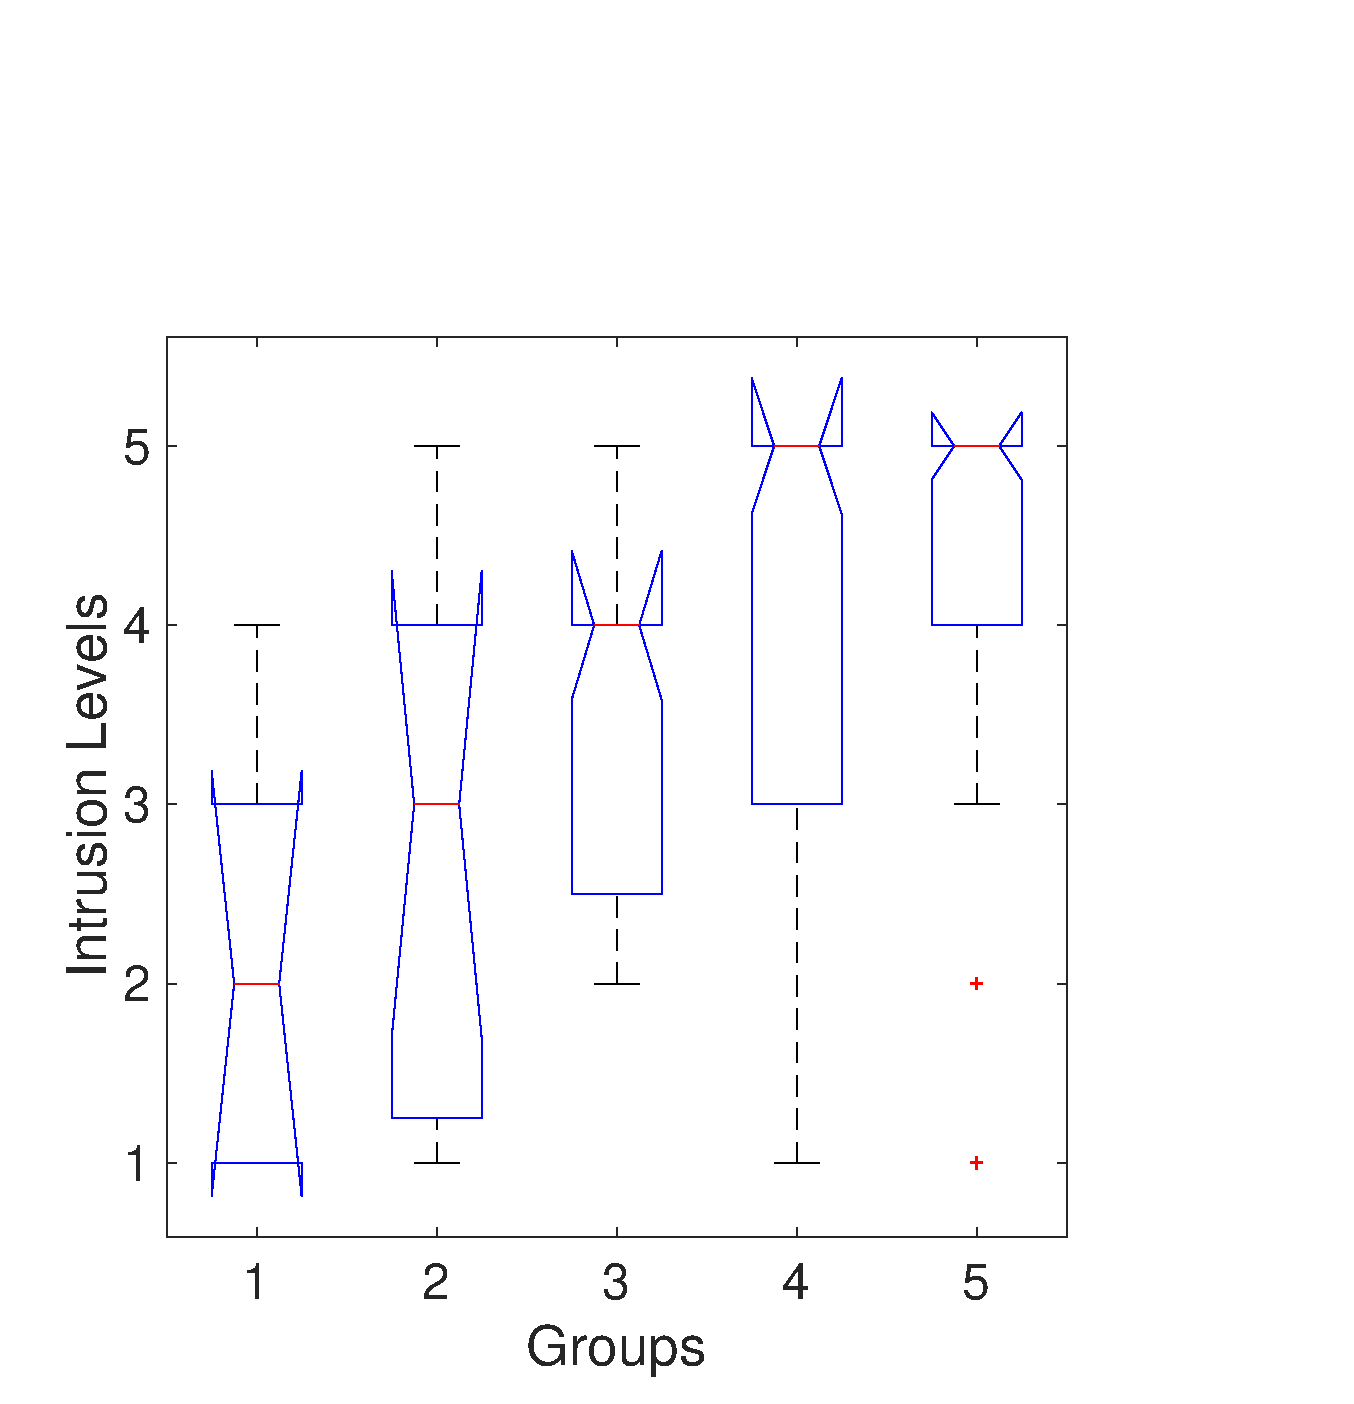
\includegraphics[width=0.5\linewidth]{./images/corp_box}}\hspace{1em}
%%\subtop[NGO\label{fig:st_ngo}]{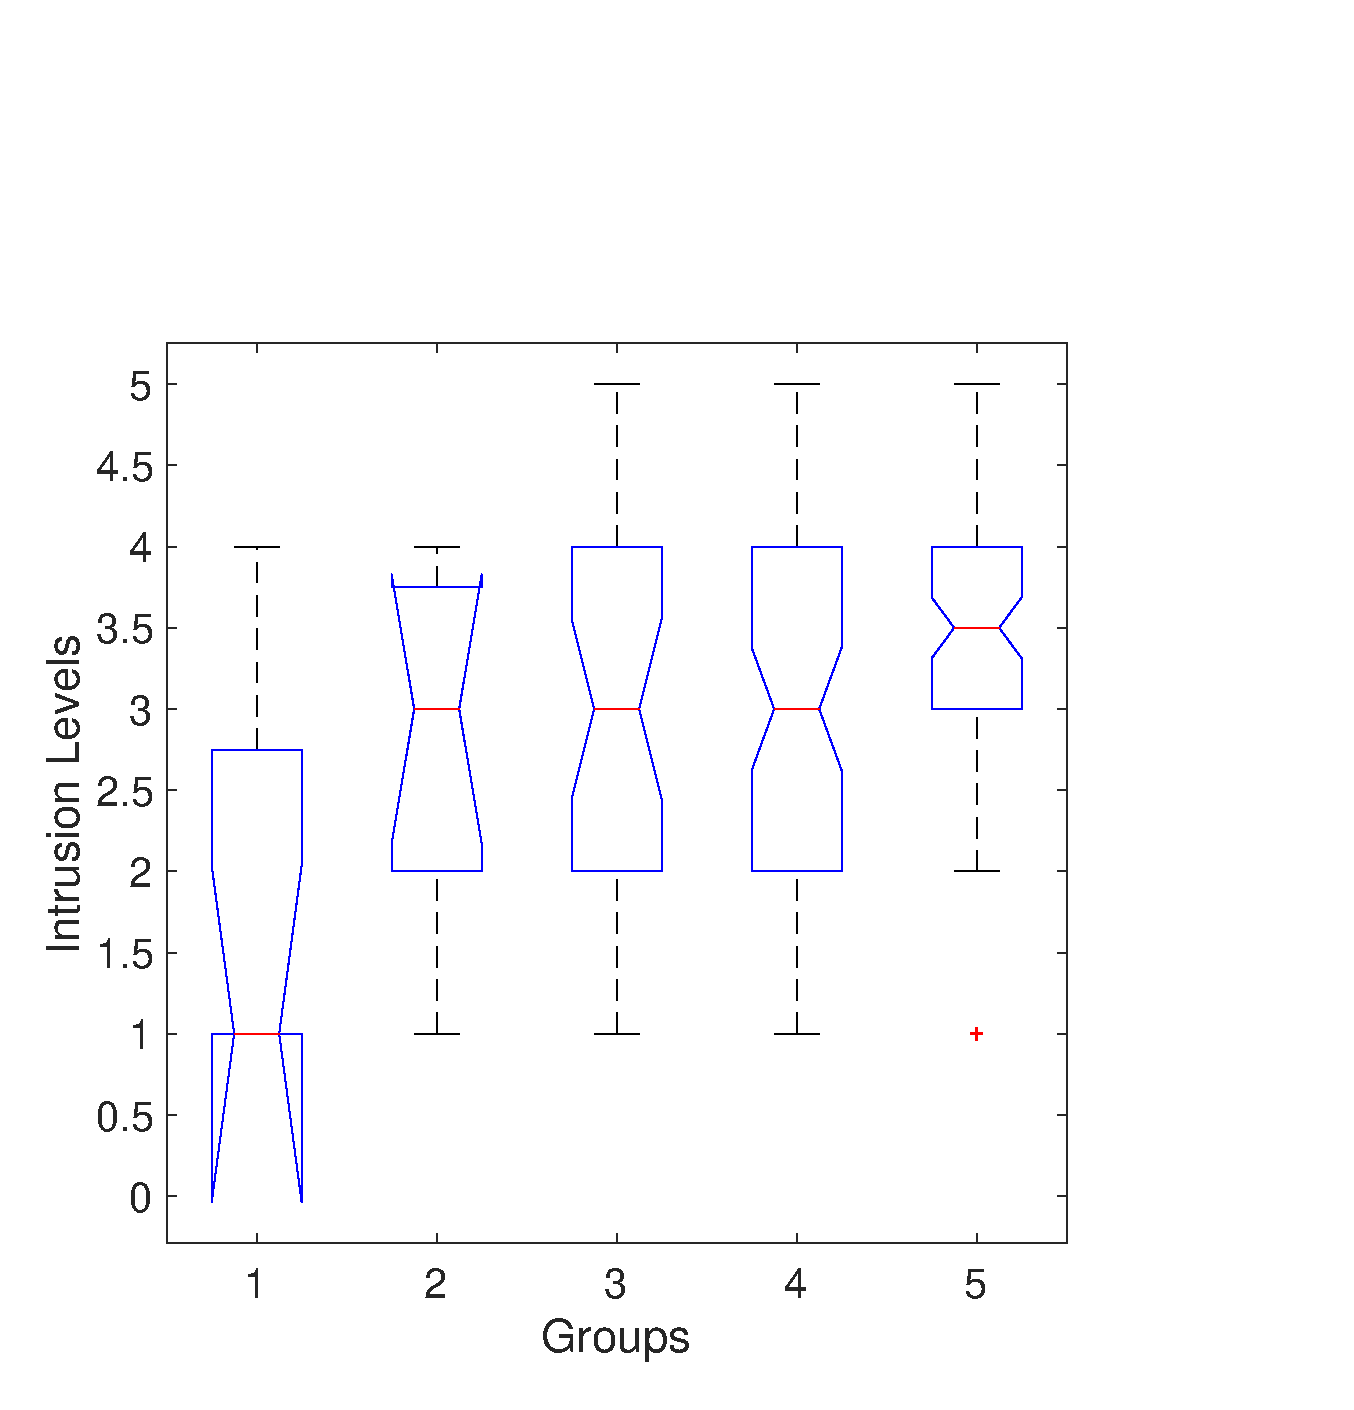
\includegraphics[width=0.5\linewidth]{./images/ngo_box}} \newline
%%\subtop[Educational Institutions\label{fig:st_edu}]{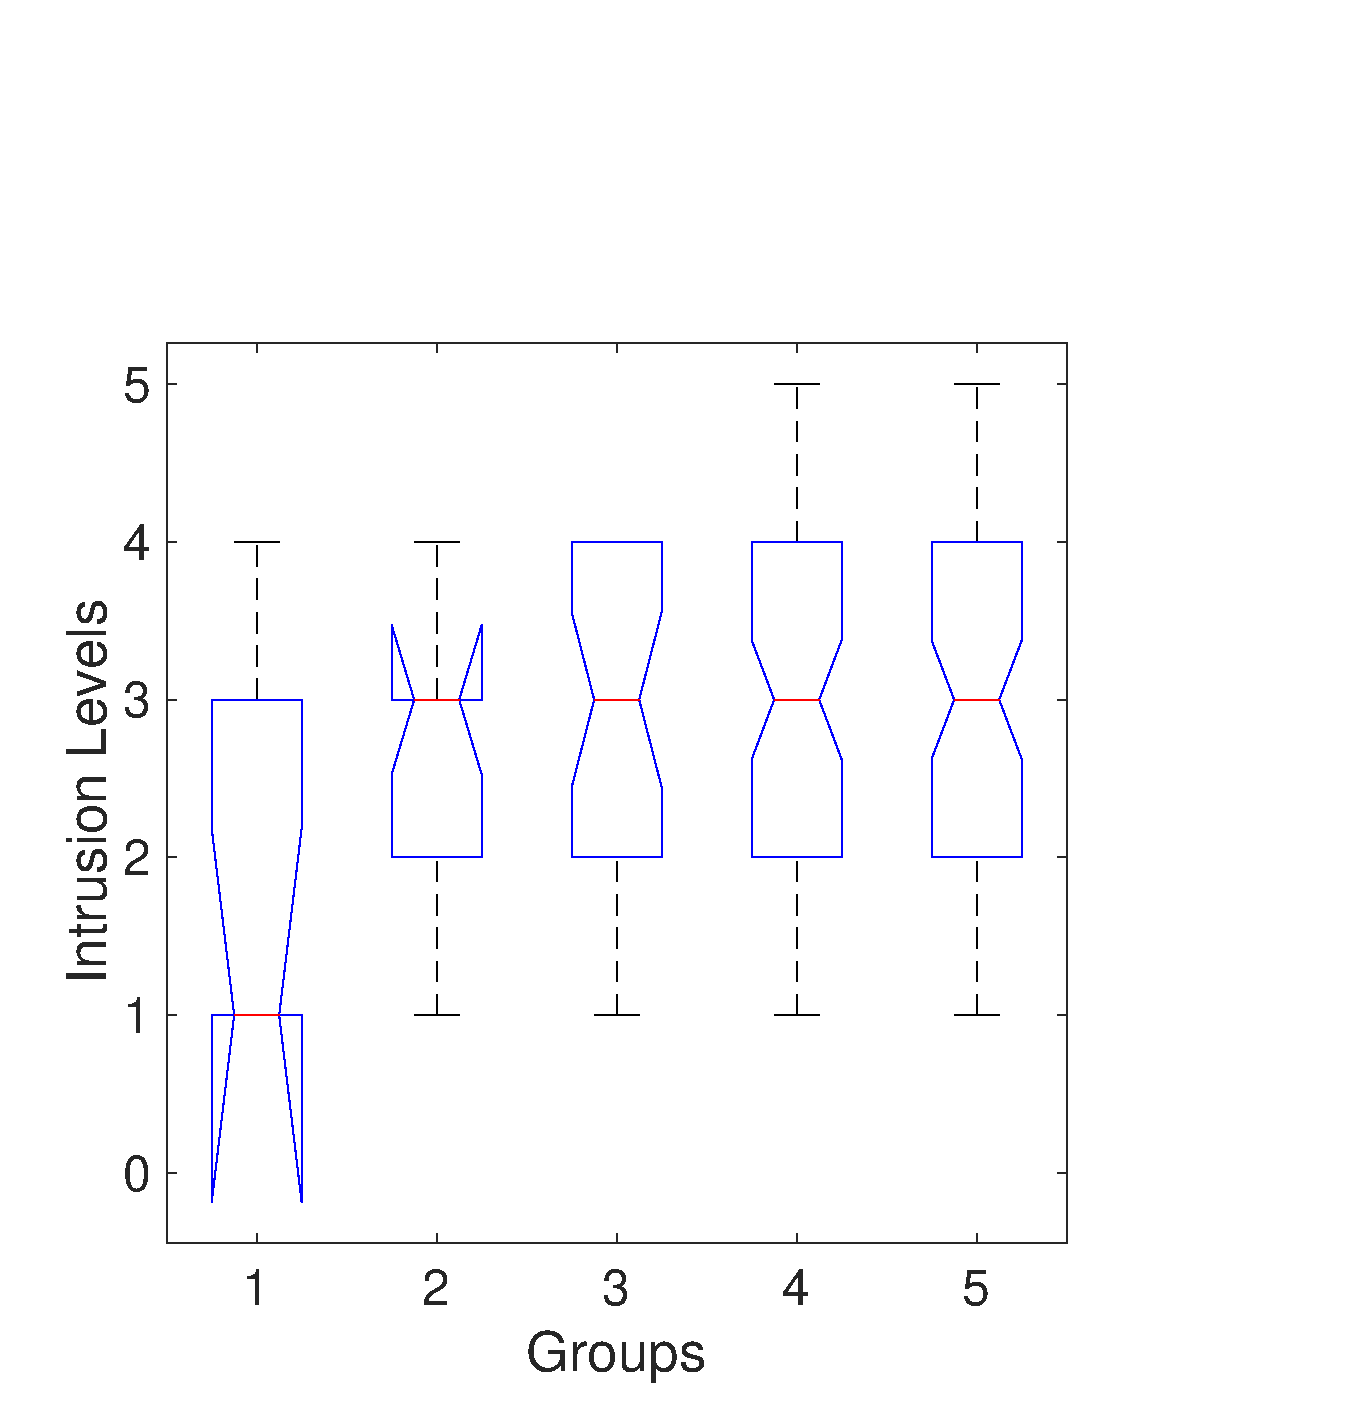
\includegraphics[width=0.5\linewidth]{./images/edu_box}}\hspace{1em}
%%\subtop[Government\label{fig:st_gov}]{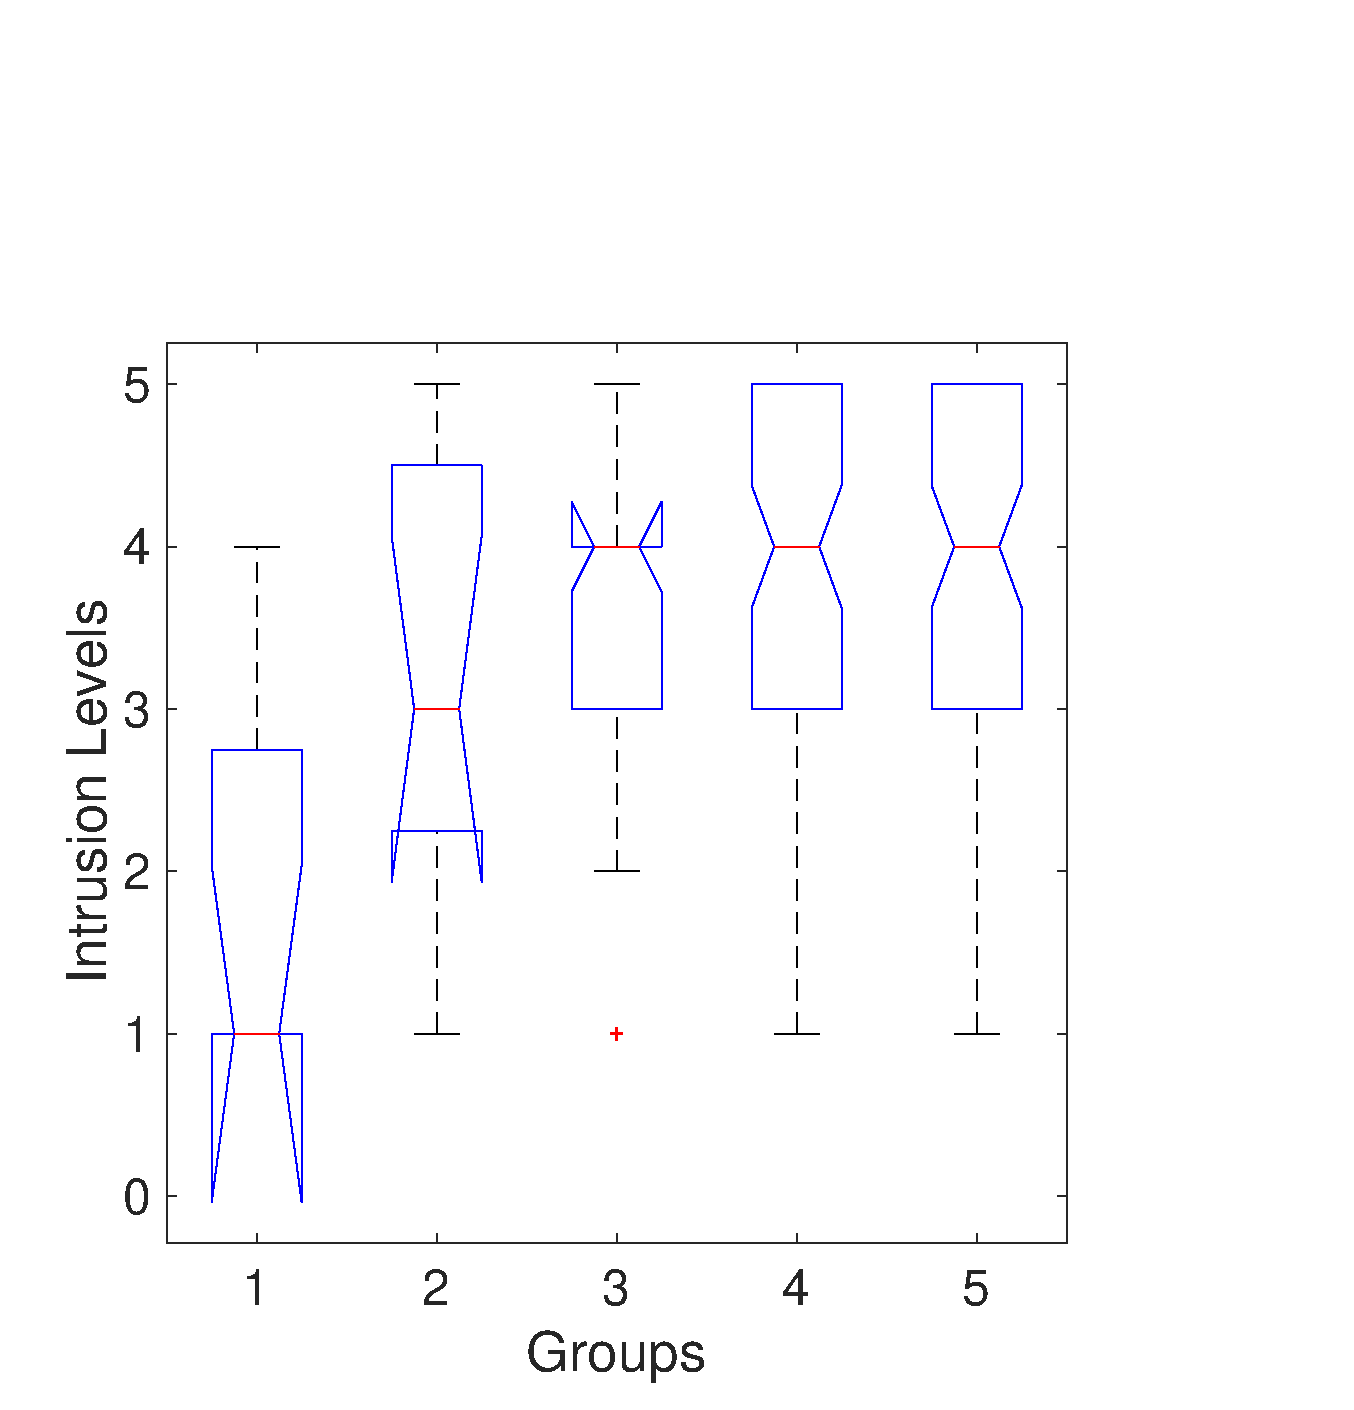
\includegraphics[width=0.5\linewidth]{./images/gov_box}} 
%%\caption{Box Plots Indicating the Population Spread of each Group}
%%\label{fig:st3}
%%\end{figure}
%%
%%\subsubsection{Perception of Individual Contexts Grouped on the Intrusion of Contexts in General}
%%
%%In this section, the relationship between the perception of contexts as a whole and the individual contexts is studied. 
%%To do this, like the above sections the data is partitioned into groups based on the answers given question 14, which asks the user the perception of intrusion of contexts in a data request. There are five groups in total partitioned using the responses given to question 14. Group one to five have each 12, 11, 42, 74 and 50 people respectively. Additional
%%information about the groups on employment, education , gender and year of birth is given in tables \ref{tab:emp_c}, \ref{tab:edu_c}, \ref{tab:gender_c} and \ref{tab:year_c}. The mean and variance of each group is shown in figures \ref{fig:co1} and \ref{fig:co2}.
%%
%%Like in the previous sections, since the data is discrete and not normal, we use the Kruskal-Wallis test to compare the groups perceptions on various contexts \ref{result:sensor}. The alpha value is considered to be 0.05. The results of the test are presented in table \ref{tab:kw_c}. As it is seen, the test says that there is a significant difference between all the groups for all contexts.
%%
%%\begin{figure}[htp]
%%\subtop[Mean of each Group for each Context\label{fig:co1}]{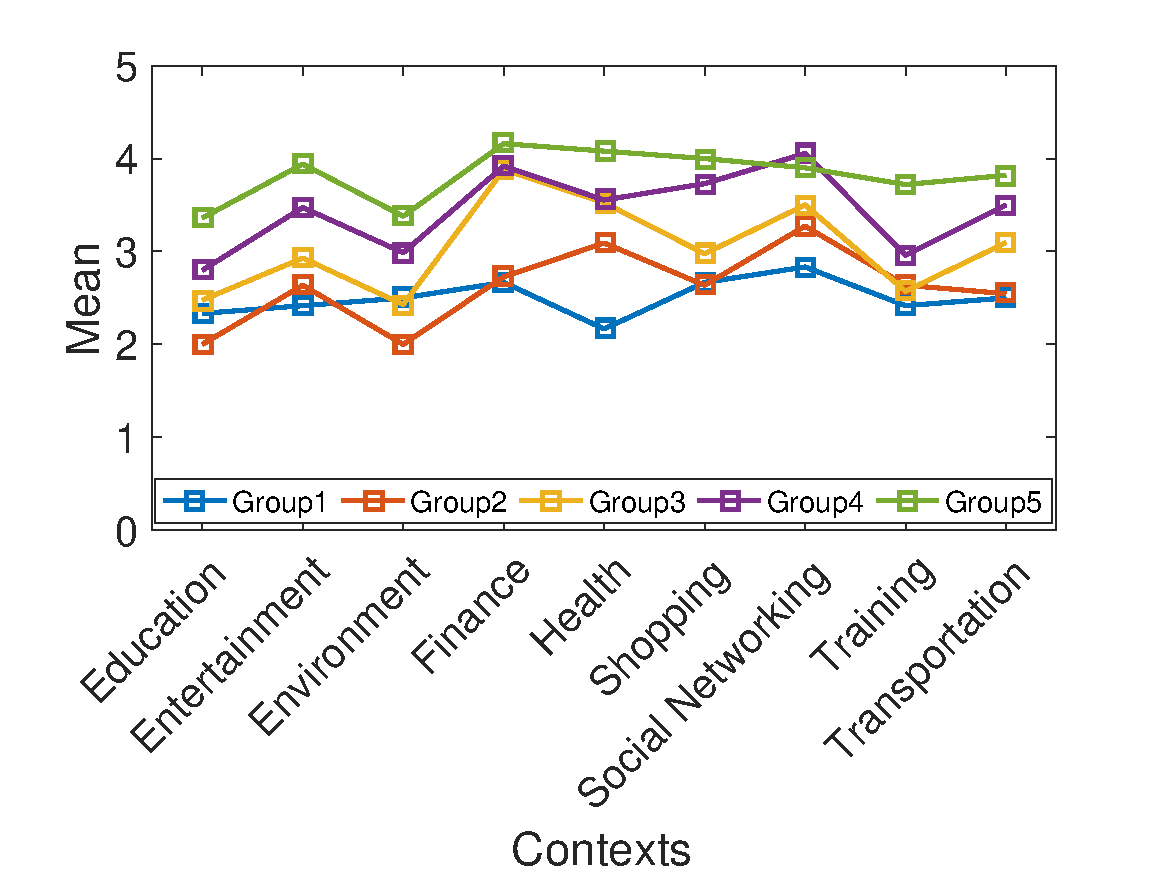
\includegraphics[width=0.5\linewidth,height=0.45\linewidth]{./images/contexts_group_meanQ14}}
%%\subtop[Variance of each Group for each Context\label{fig:co2}]{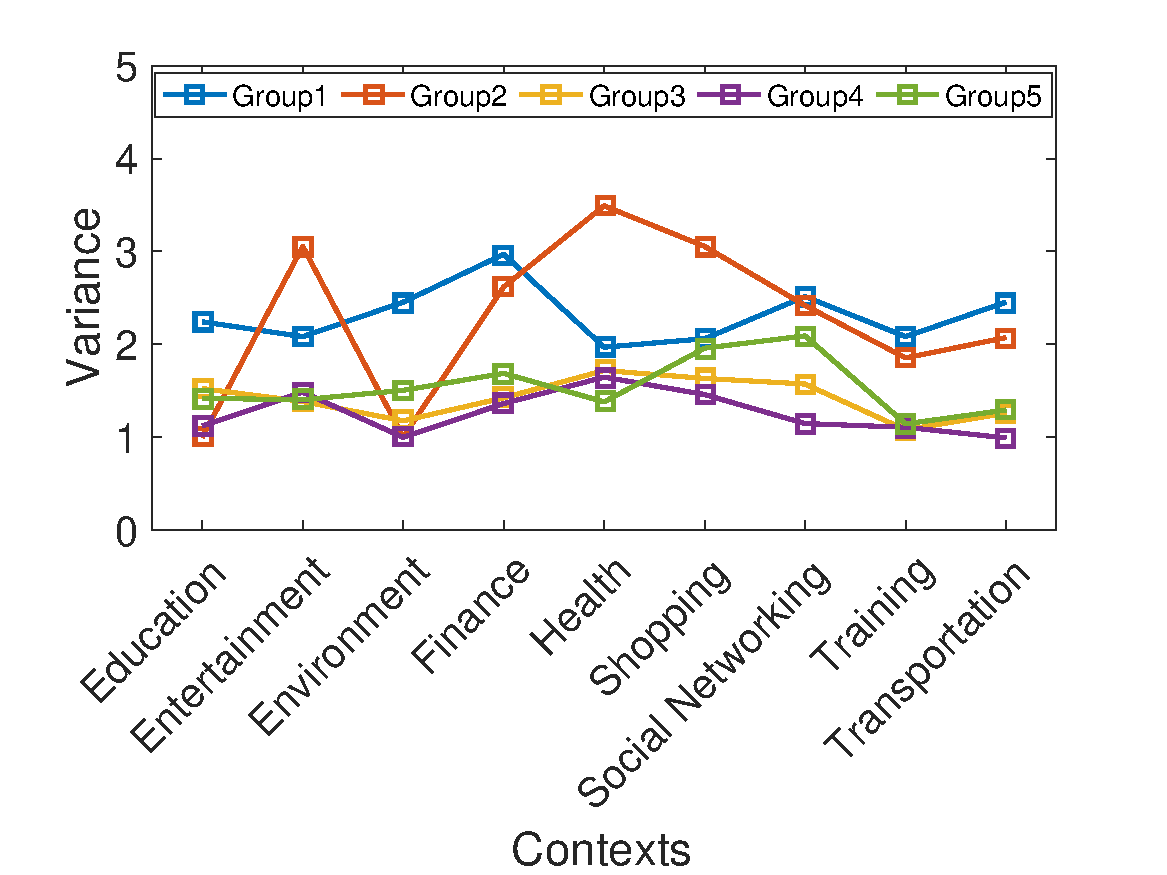
\includegraphics[width=0.5\linewidth,height=0.45\linewidth]{./images/contexts_group_varianceQ14}}
%%\caption{Mean and Variance of Groups}
%%\label{fig:co3}
%%\end{figure}
%%
%%\begin{table}[h!]
%%  \centering
%%  \caption{Kuskal-Wallis Test for Contexts}
%%  \label{tab:kw_c}
%%  \begin{tabular}{cc}
%%    \toprule
%%     Context & p-value \\
%%    \midrule
%%    Education &  6.4694e-04 \\
%%    Entertainment & 1.0660e-04\\
%%    Environment & 1.3079e-04\\
%%    Finance & 0.0021\\ 
%%    Health & 0.0011\\
%%    Shopping & 5.4227e-05\\ 
%%    Social Network &  0.0120\\
%%    Training & 1.2071e-05\\
%%    Transportation & 4.9043e-04\\ 
%%    \bottomrule
%%  \end{tabular}
%%\end{table} 
%%
%%Dunn's Test is performed as a post hoc test for all the contexts to observe the exact group pairs that might be significantly different. The results are presented in tables \ref{tab:dunn_c} and \ref{tab:dunn_c1}. 
%%
%%For the context education, the groups (2,5) and (3,5) are significantly different from each other. The figure \ref{fig:co_educ} shows the spread of the groups. It is seen that groups with larger difference in opinion about contexts have larger differences in opinion about the context education. The reason why the group 1 was not significantly different from group 5 can be attributed to the fact that the population of the survey might not be a representative sample. Secondly, the number of participants in the survey is limited to 189. Thirdly, due to the previous statement the number of people in group 1 is just 12 and the population sample can be unrepresentative of the actual distribution.
%%
%%For the context entertainment, further investigation shows that groups (1,5), (2,5) and (3,5) are significantly different in each others responses. The figure \ref{fig:co_ent} shows the spread of the groups. Therefore, we infer that groups with higher differences in opinions about contexts (such as groups 1 and 5) have varying opinions of intrusion on entertainment.
%%
%%For the context environment, groups (2,5) and (3,5) are significantly different from each other. The figure \ref{fig:co_env} shows the spread of the groups. We can come to a similar conclusion as to the context education as to why group 1 is not significantly different from group 5.
%%
%%For the context finance, the groups (1,5), and (2,5) are significantly different from each other. The figure \ref{fig:co_finance} shows the spread of the groups and we can infer that groups with bigger differences in opinions on contexts also have significant differences in their opinions on finance context.
%%
%%In the context health, except for groups (1,5) all the other groups are not significantly different from each other. The figure \ref{fig:co_health} shows the spread of the groups and we can infer people who find contexts non intrusive and very intrusive have significant difference in viewpoint of the health context. As seen, all the other groups have significant overlap with groups 1 and 5.
%%
%%For the context shopping and social network, none of the groups are significantly different from each other as seen in \ref{fig:co_shopping}. This show that irrespective of their viewpoint about contexts, all groups have similar opinions with the context shopping and social network.
%%
%%In the context training, the groups (1,5),(3,5) and (4,5) are significantly different from each other. The figure \ref{fig:co_training} shows the spread of the groups. This show that all groups have similar opinions about training contexts except for group 5. The reason for group 2 not being different from group 5 is due to the small population size of group 2. Additional points are mentioned for the context education.
%%
%%Finally for the context transportation, the groups (1,5), (2,5) and (3,5) are significantly different from each other. It is seen in figure \ref{fig:co_nav} that groups 1,2,3 are significantly different form group 5. Group 4 is not significantly different from group 5 due to the fact that the users of group 4 and 5 have closer opinions of contexts than the rest. Hence users who find contexts intrusive will have a significant difference in opinion with sufficiently different groups.
%%
%%This goes to show that groups that perceive contexts in a more different light tend to have different ways of viewing the individual contexts. We do observe that in some cases (2,5) are significantly different, but (1,5) is not. This can be attributed to the low number of responses
%%and the noise in the data. 
%%
%%Shopping and social networking are considered highly intrusive with values 3.75 and 3.50 and every group had similar opinions. Finance and health are also very intrusive with levels 3.85 and 3.60 on a scale of five. Here a significant difference in opinions was observed between groups with largely different opinions about contexts in general (such as group 1 and 5).
%%
%%Education and environment are considered 2.83 and 2.92 intrusive on a scale of five, which are the lowest. For these two we observe that there is a significant difference between groups 2 with 5 and 3 with 5. For entertainment and transportation which have medium intrusion levels of 3.39 and 3.38 on a scale of five and it is observed that groups 1, 2, 3 differ significantly from group 5. It is still observed that groups with higher intrusion perception of contexts (such as group 5) view some contexts in a more intrusive light and should be incentivized more for those.
%%
%%\begin{table}[h!]
%%  \centering
%%  \caption{Dunn's Test for Contexts Part 1}
%%  \label{tab:dunn_c}
%%  \begin{tabular}{cccccccc}
%%    \toprule
%%     Groups & Education & Entertainment & Environment & Finance & Health  \\
%%    \midrule
%%    (1,2)&0.99796&0.99982&0.97055&1.0000&0.63908\\
%%(1,3)&1.0000&0.99174&1&0.32963&0.076147\\
%%(1,4)&0.94148&0.19262&0.86998&0.22077&0.042547\\
%%(1,5)&0.11471&0.0056283&0.21553&0.015364&0.00051115\\
%%(2,3)&0.9342&1&0.96665&0.31604&0.9999\\
%%(2,4)&0.32744&0.76121&0.083389&0.21508&0.99963\\
%%(2,5)&0.0082212&0.082023&0.0048936&0.016365&0.50246\\
%%(3,4)&0.83617&0.23034&0.10875&1.0000&1.0000\\
%%(3,5)&0.0064191&0.00086418&0.0012905&0.65747&0.32713\\
%%(4,5)&0.13825&0.28231&0.60016&0.57519&0.21258\\
%%    \bottomrule
%%  \end{tabular}
%%\end{table}
%%
%%\begin{table}[h!]
%%  \centering
%%  \caption{Dunn's Test for Contexts Part 2}
%%  \label{tab:dunn_c1}
%%  \begin{tabular}{ccccccc}
%%    \toprule
%%     Groups & Shopping & Social Network & Training & Transportation  \\
%%    \midrule
%%(1,2) &1.0000&0.99831&1.0000&1.0000\\
%%(1,3)&0.99992&0.94767&1.0000&0.9722\\
%%(1,4)&0.18309&0.089135&0.90197&0.23809\\
%%(1,5)&0.015842&0.10636&0.010906&0.016376\\
%%(2,3)&1.0000&1.0000&1&0.98253\\
%%(2,4)&0.39426&0.70552&0.99778&0.30509\\
%%(2,5)&0.052334&0.7272&0.068368&0.026144\\
%%(3,4)&0.038351&0.21259&0.58123&0.51397\\
%%(3,5)&0.00050454&0.29374&2.1697e-05&0.012924\\
%%(4,5)&0.69535&1.0000&0.0033189&0.55629\\
%%\bottomrule
%%  \end{tabular}
%%\end{table} 
%%
%%
%%\begin{figure}[htp]
%%
%%\subtop[Education\label{fig:co_educ}]{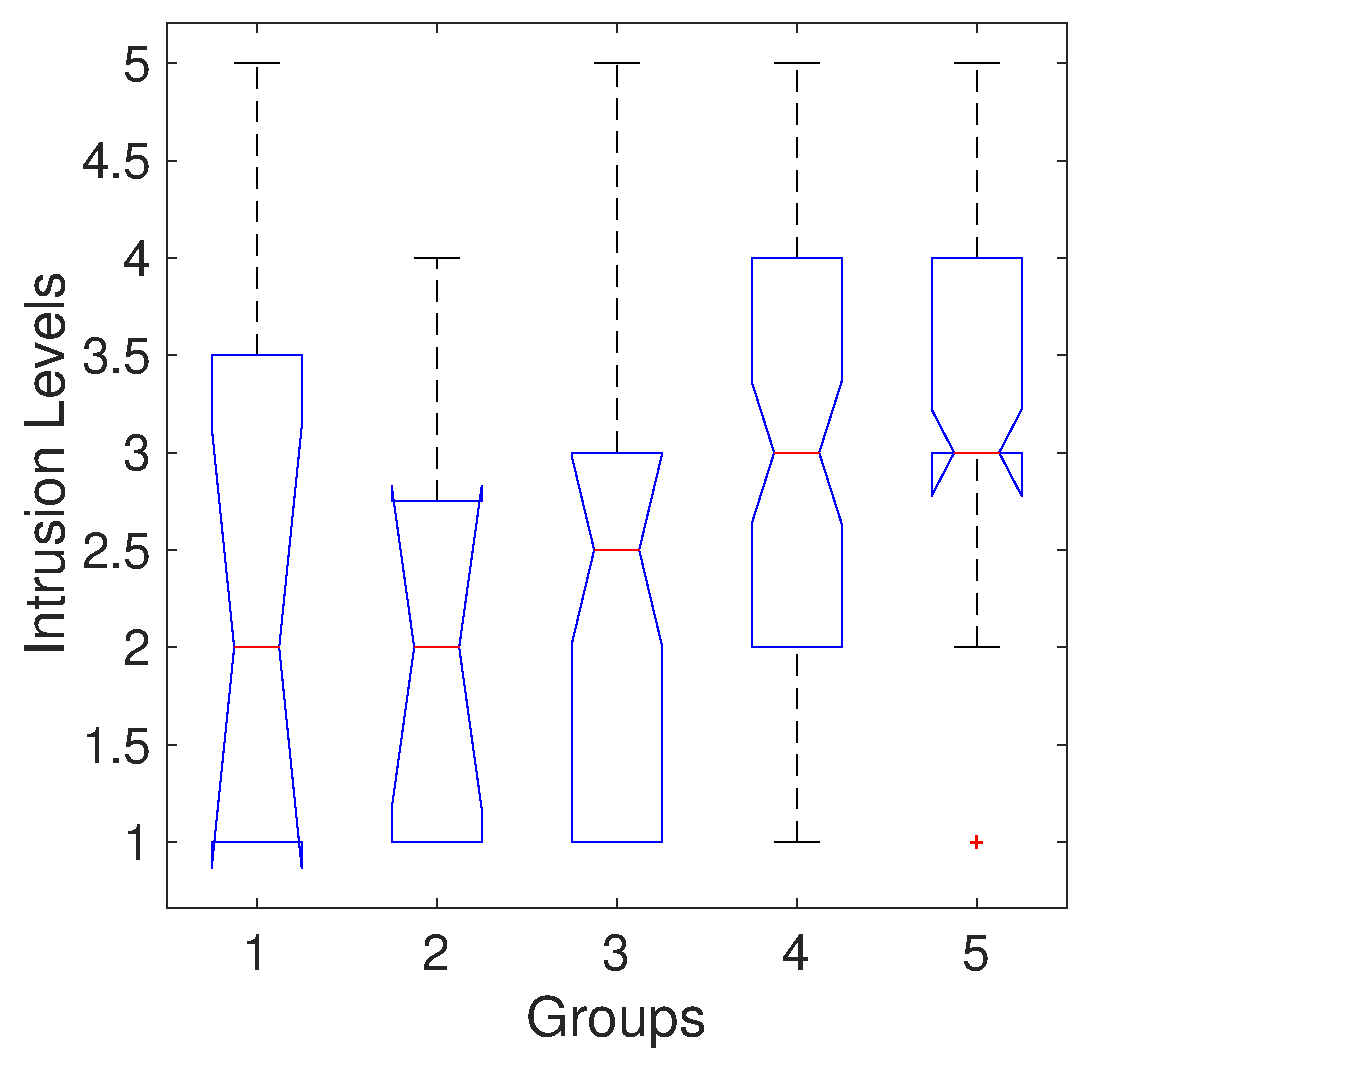
\includegraphics[width=0.5\linewidth]{./images/educ_box}}\hspace{1em}
%%\subtop[Entertainment\label{fig:co_ent}]{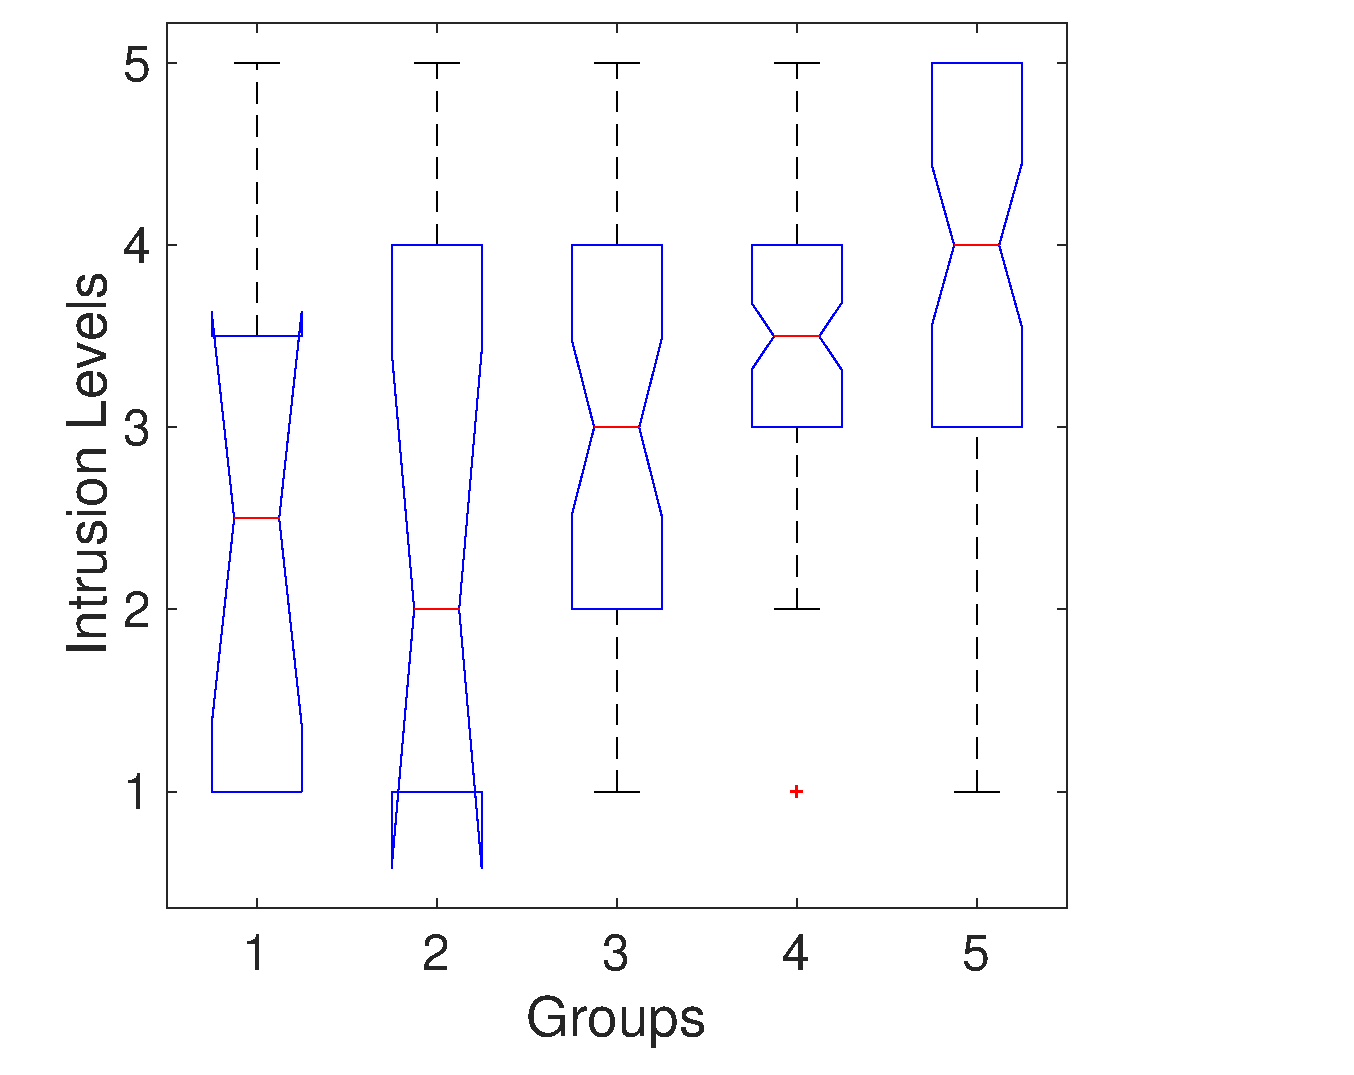
\includegraphics[width=0.5\linewidth]{./images/ent_box}} \newline
%%\subtop[Environment\label{fig:co_env}]{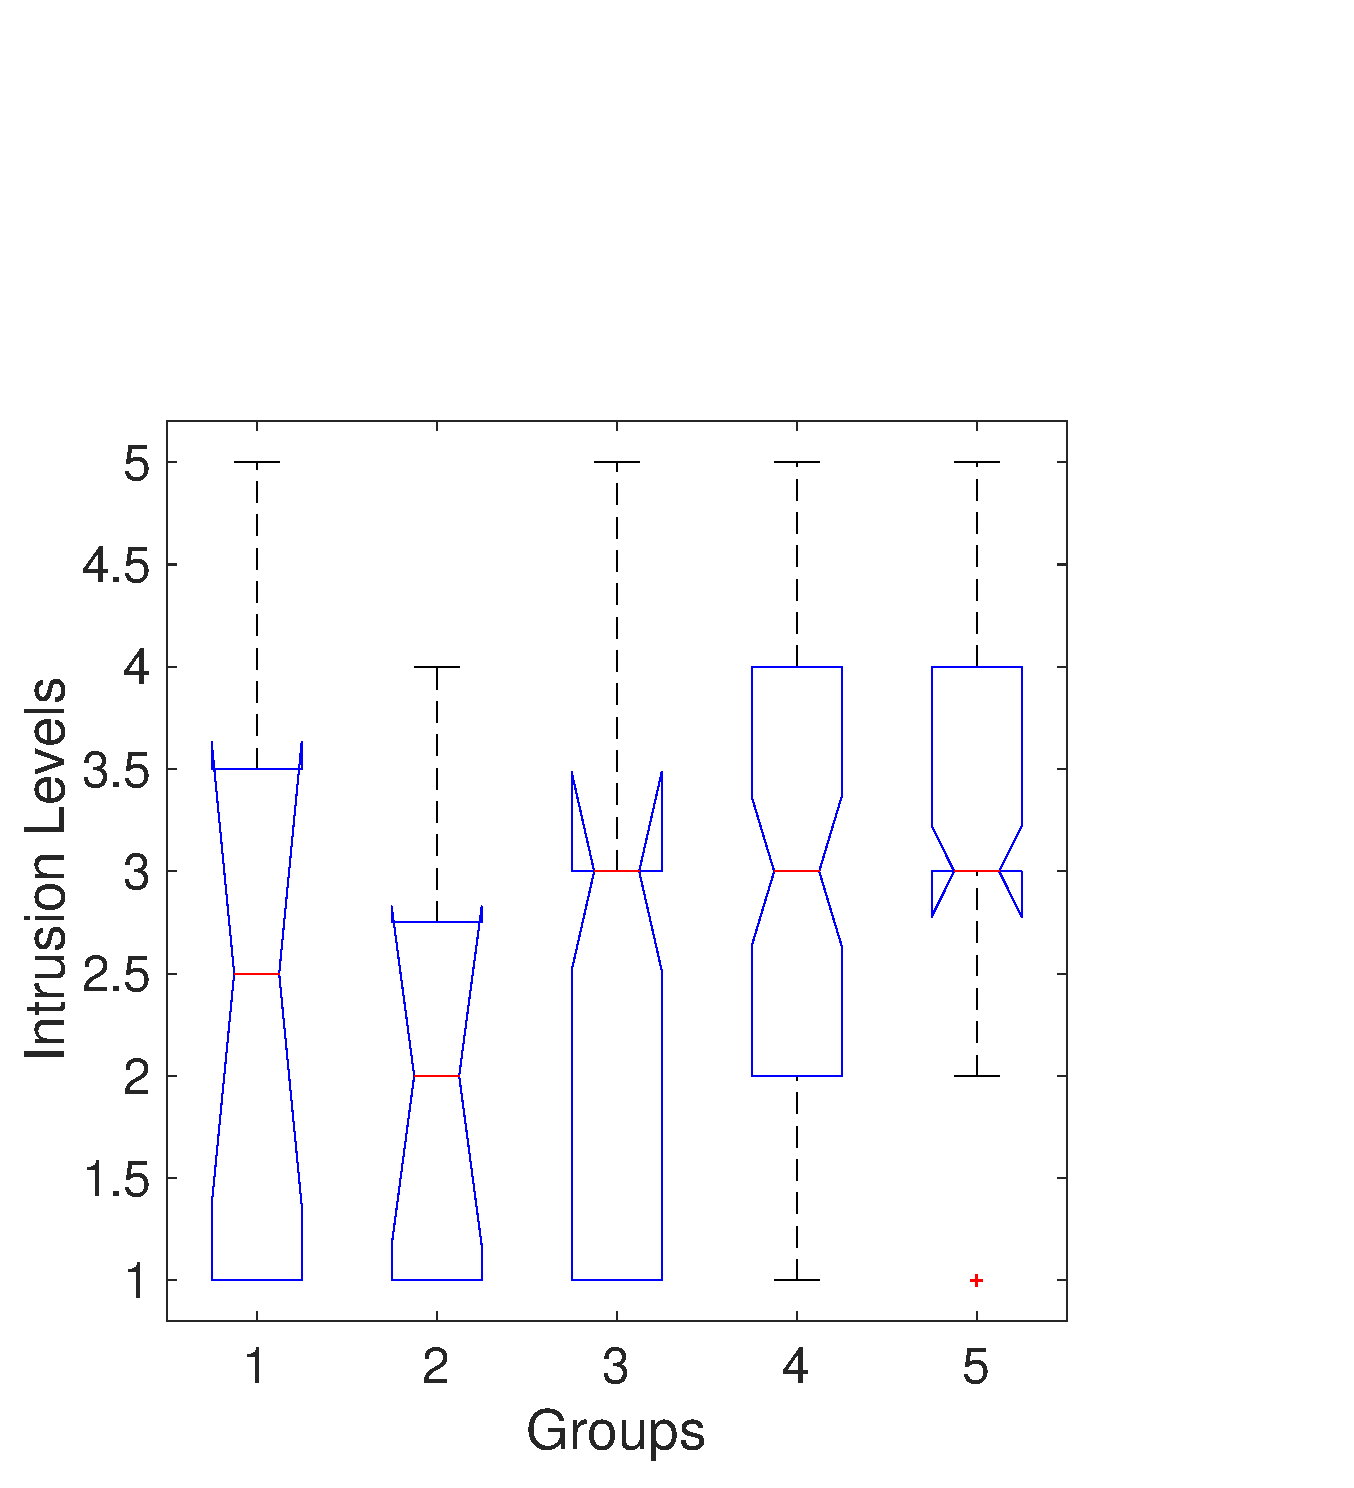
\includegraphics[width=0.5\linewidth]{./images/env_box}}\hspace{1em}
%%\subtop[Finance\label{fig:co_finance}]{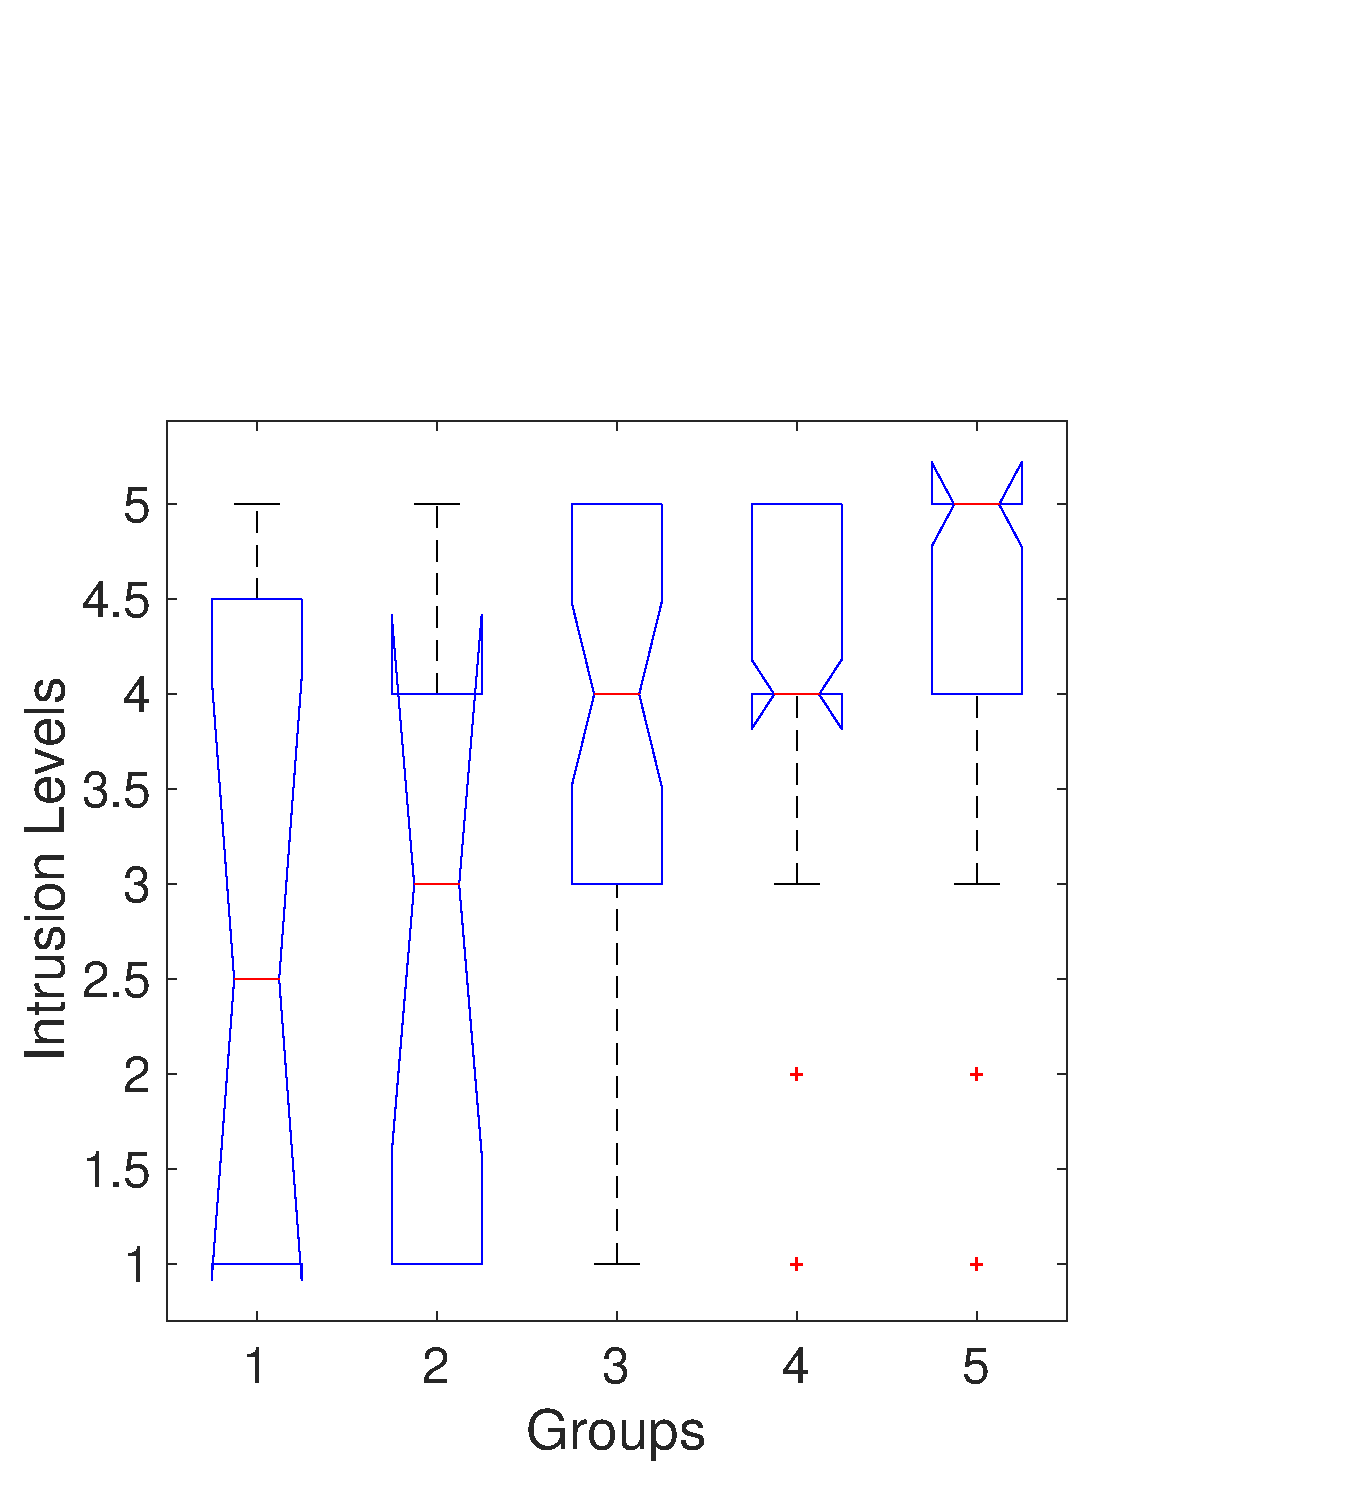
\includegraphics[width=0.5\linewidth]{./images/finance_box}} \newline
%%\subtop[Health\label{fig:co_health}]{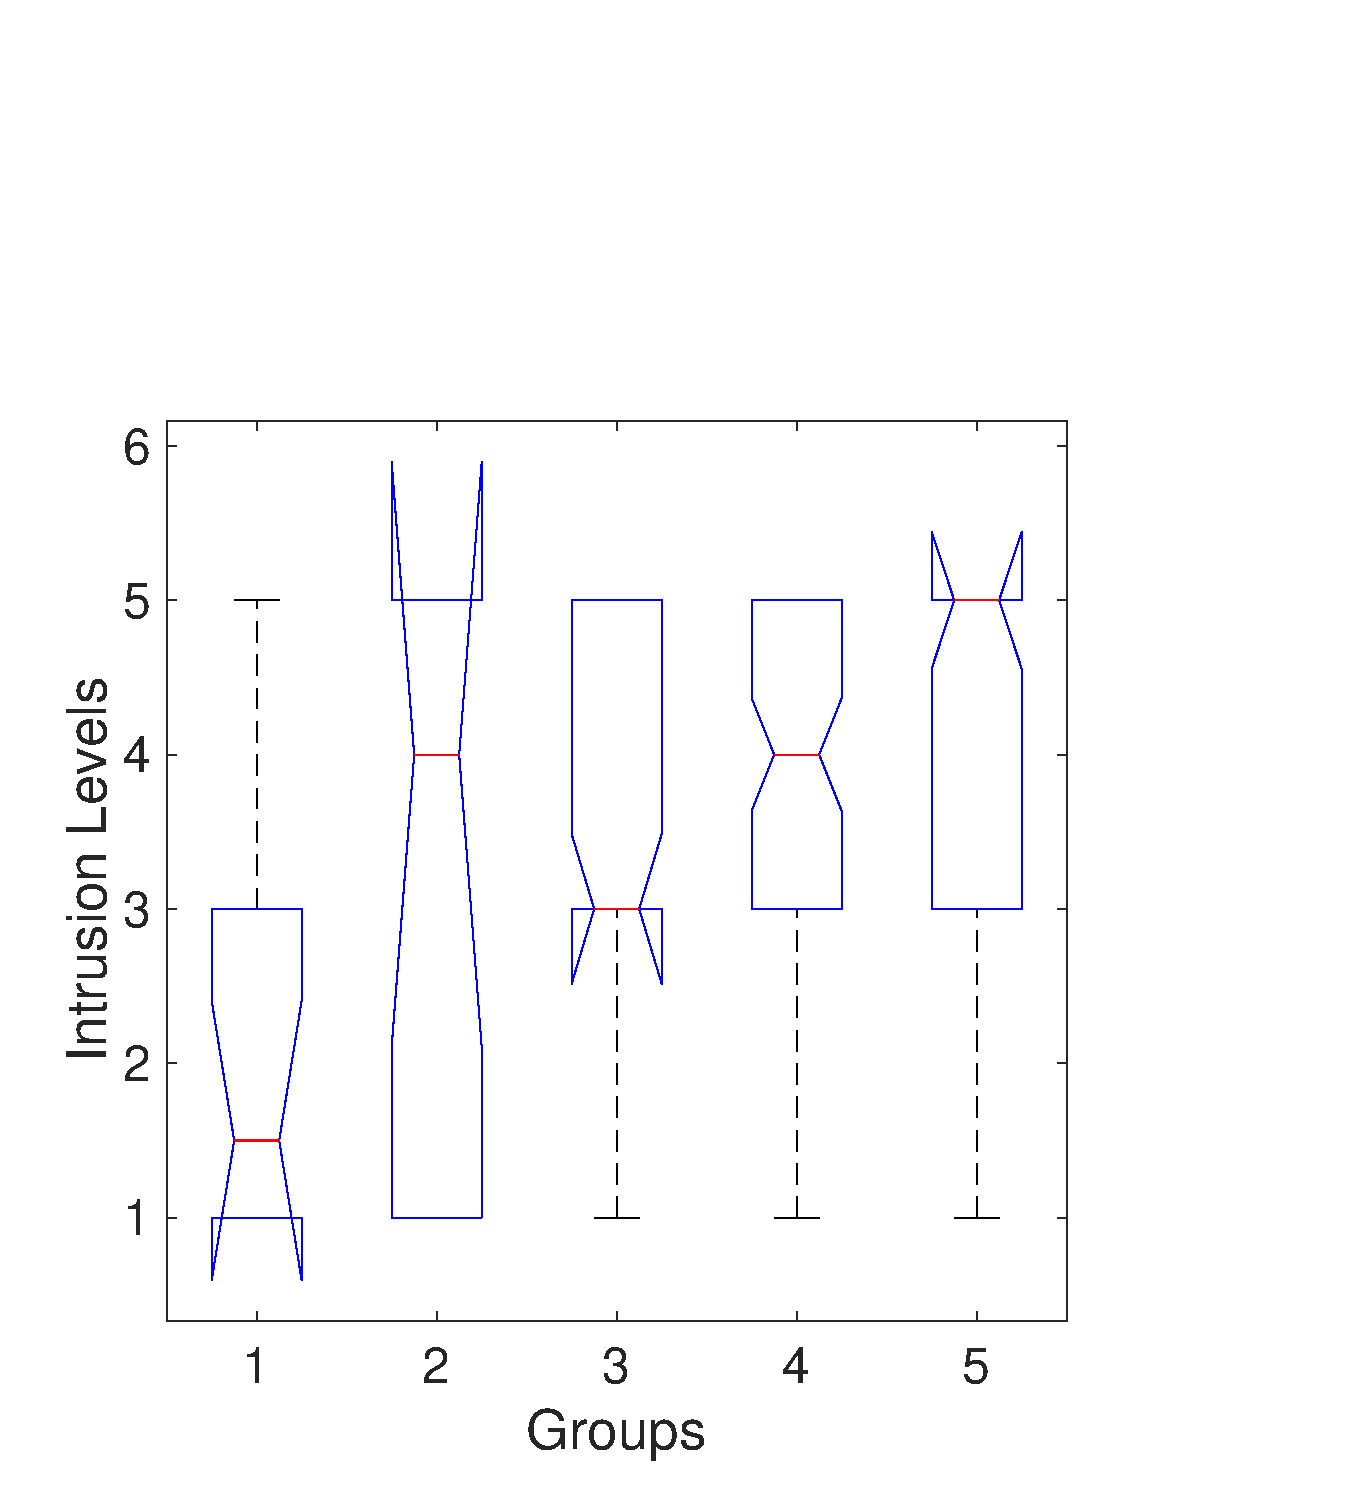
\includegraphics[width=0.5\linewidth]{./images/health_box}}\hspace{1em}
%%\subtop[Shopping\label{fig:co_shopping}]{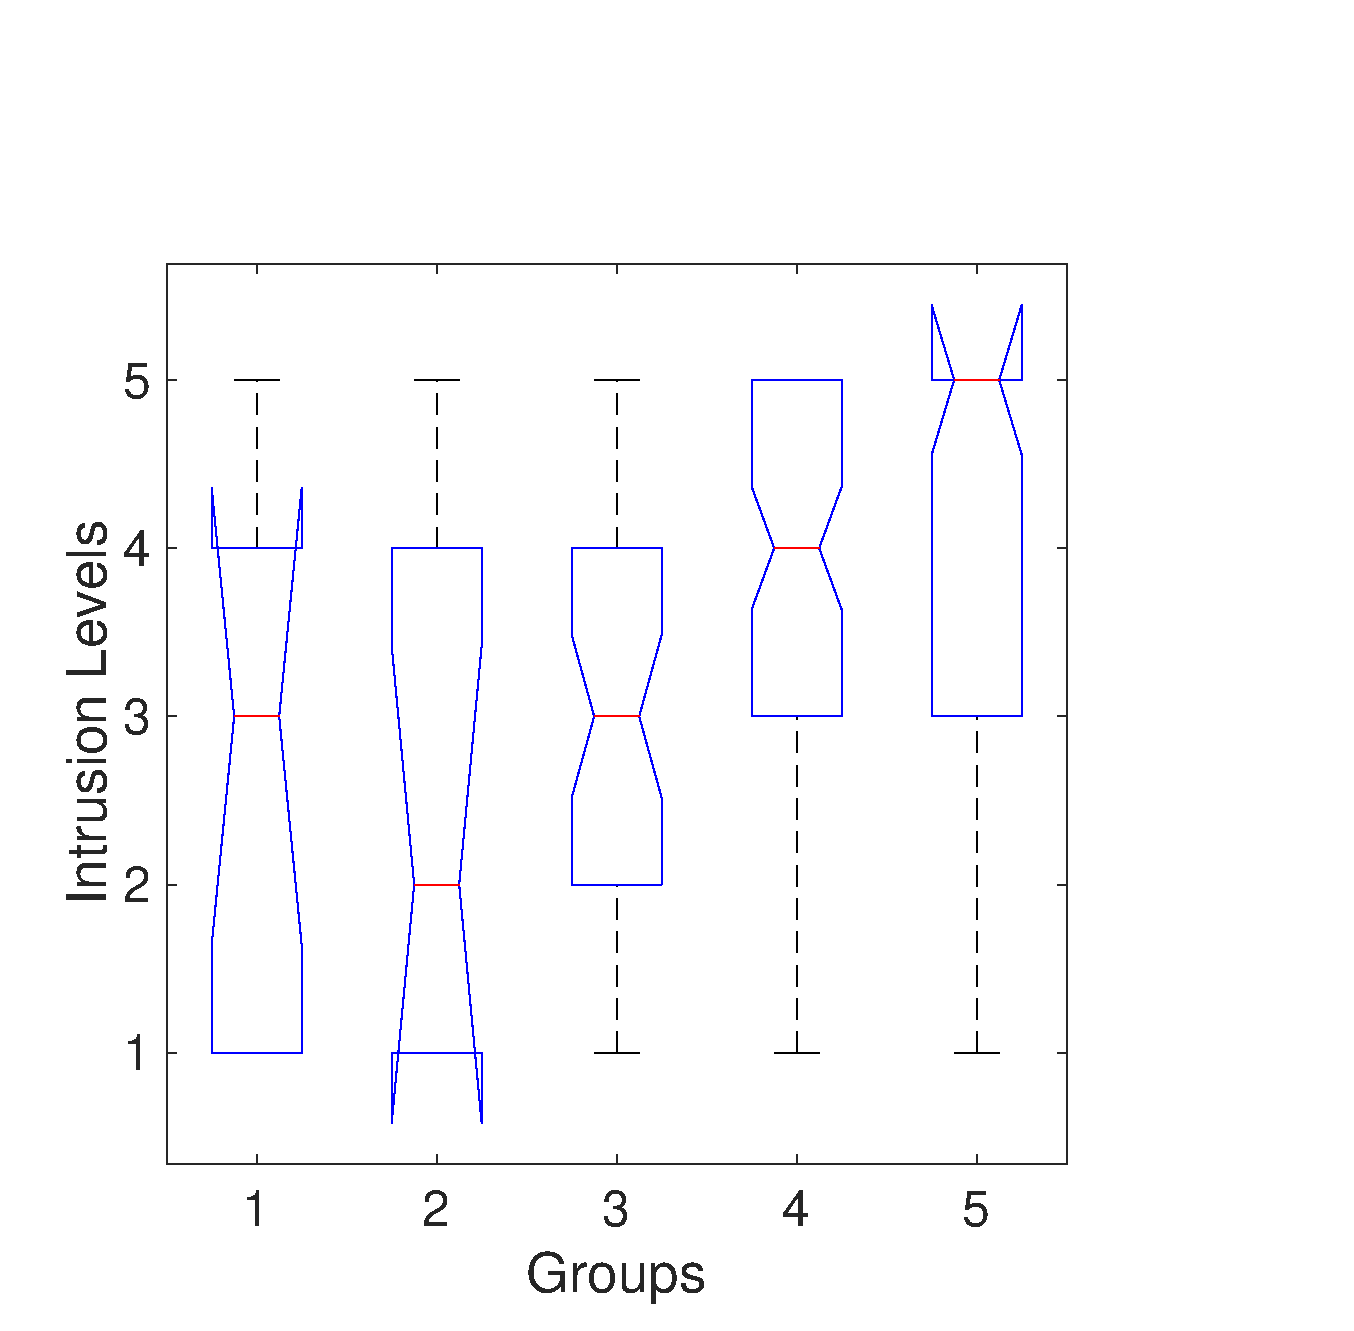
\includegraphics[width=0.5\linewidth]{./images/shopping_box}} 
%%\caption{Mean and Variance of Groups}
%%\label{fig:st3}
%%\end{figure}
%%
%%\begin{figure}[htp]
%%\subtop[Social Networking\label{fig:co_social}]{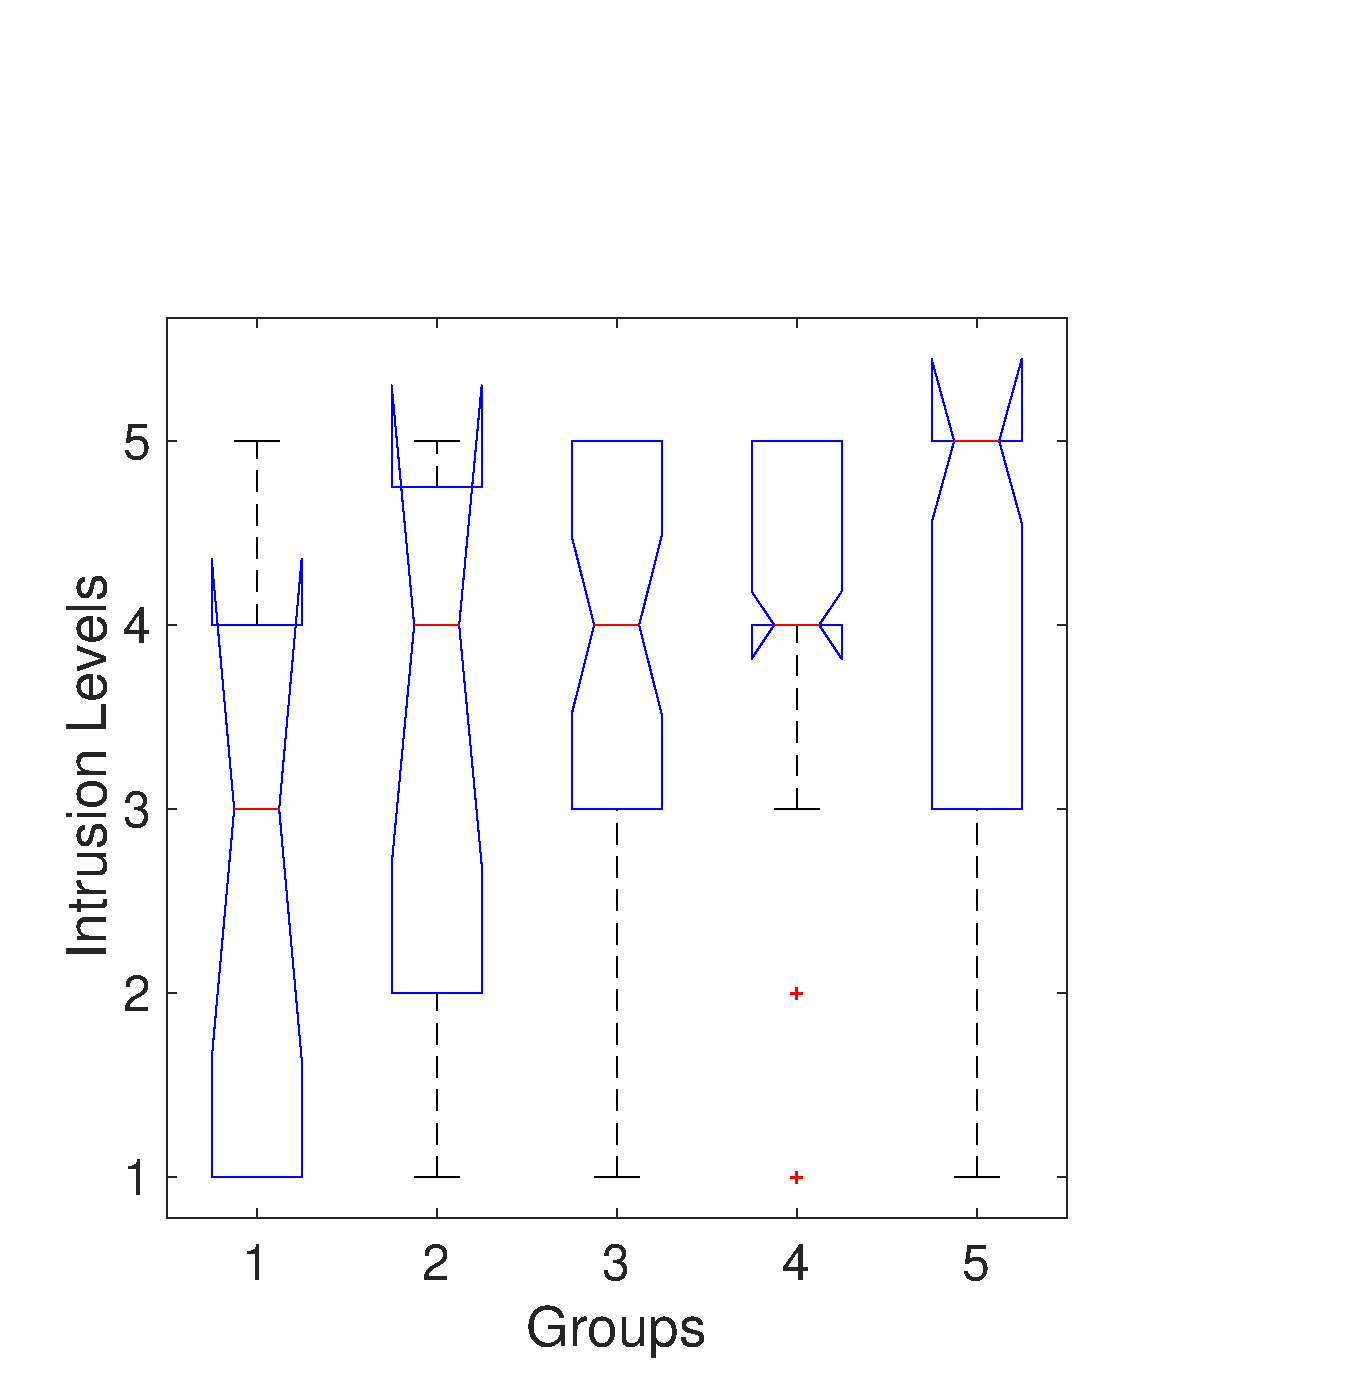
\includegraphics[width=0.47\linewidth]{./images/social_box}}\hspace{1em}
%%\subtop[Training\label{fig:co_training}]{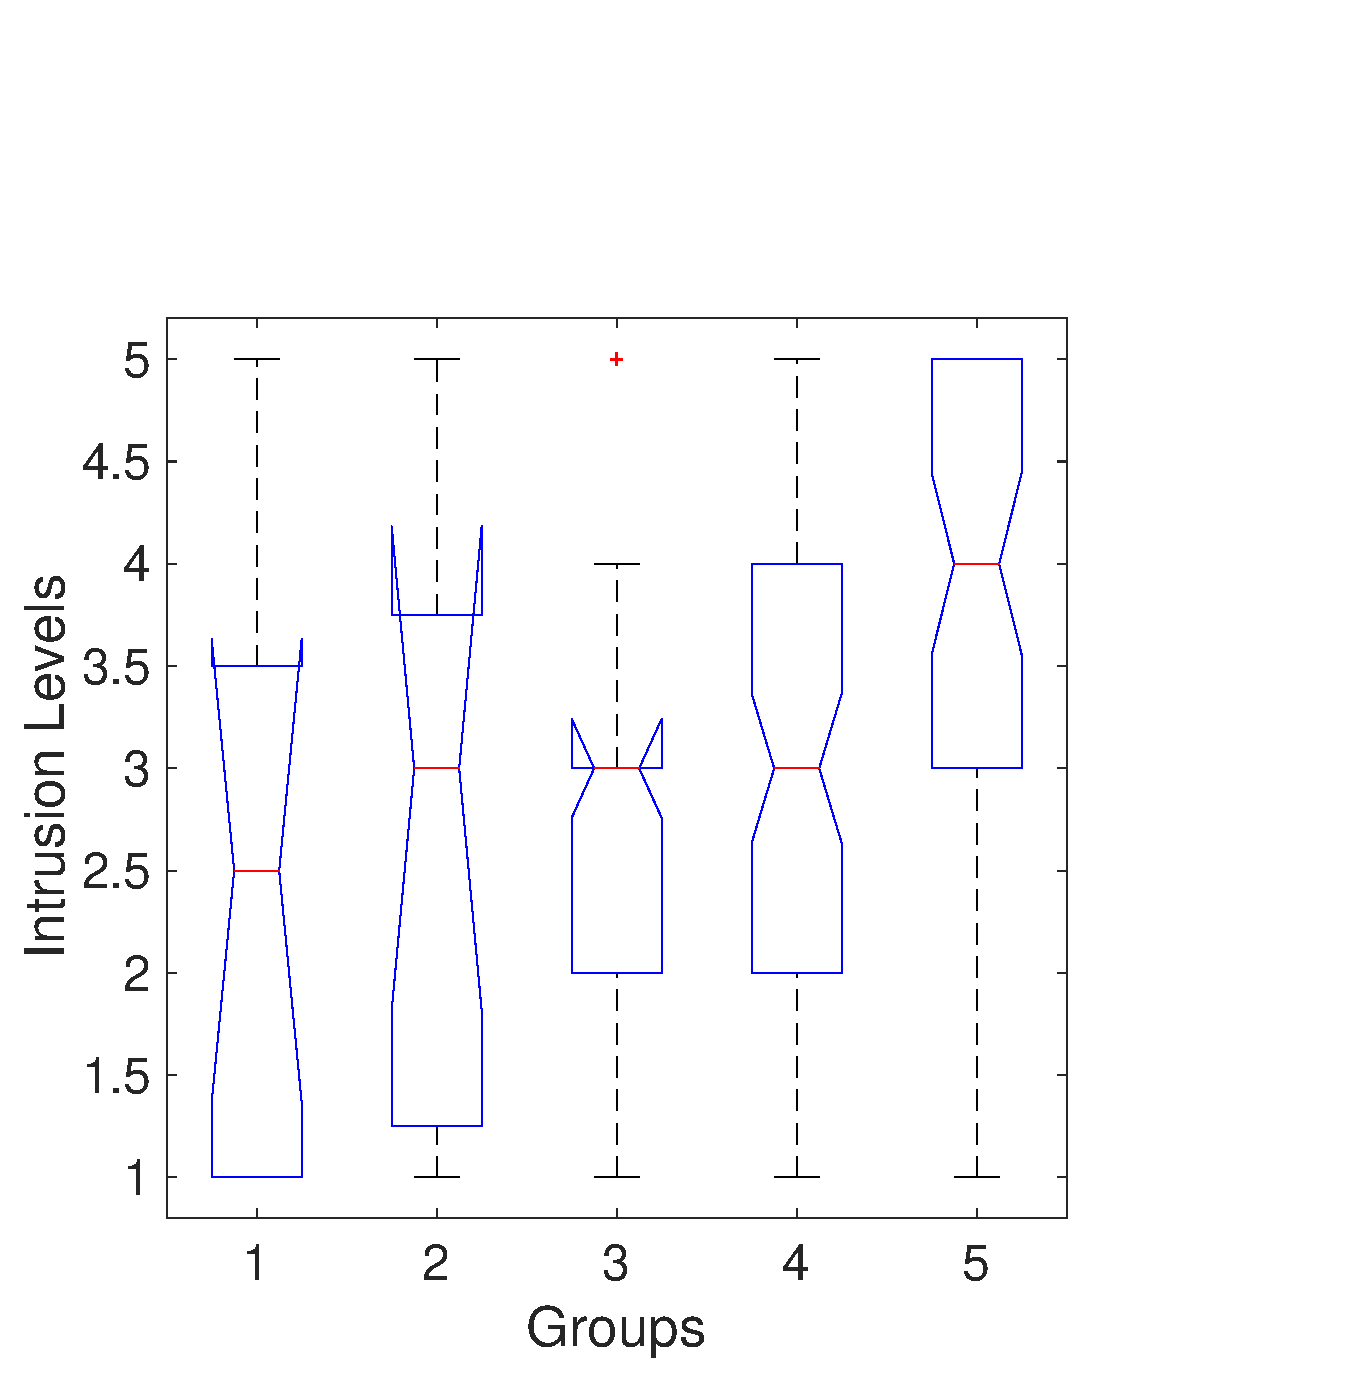
\includegraphics[width=0.47\linewidth]{./images/training_box}}\newline
%%\centering
%%\subtop[Navigation\label{fig:co_nav}]{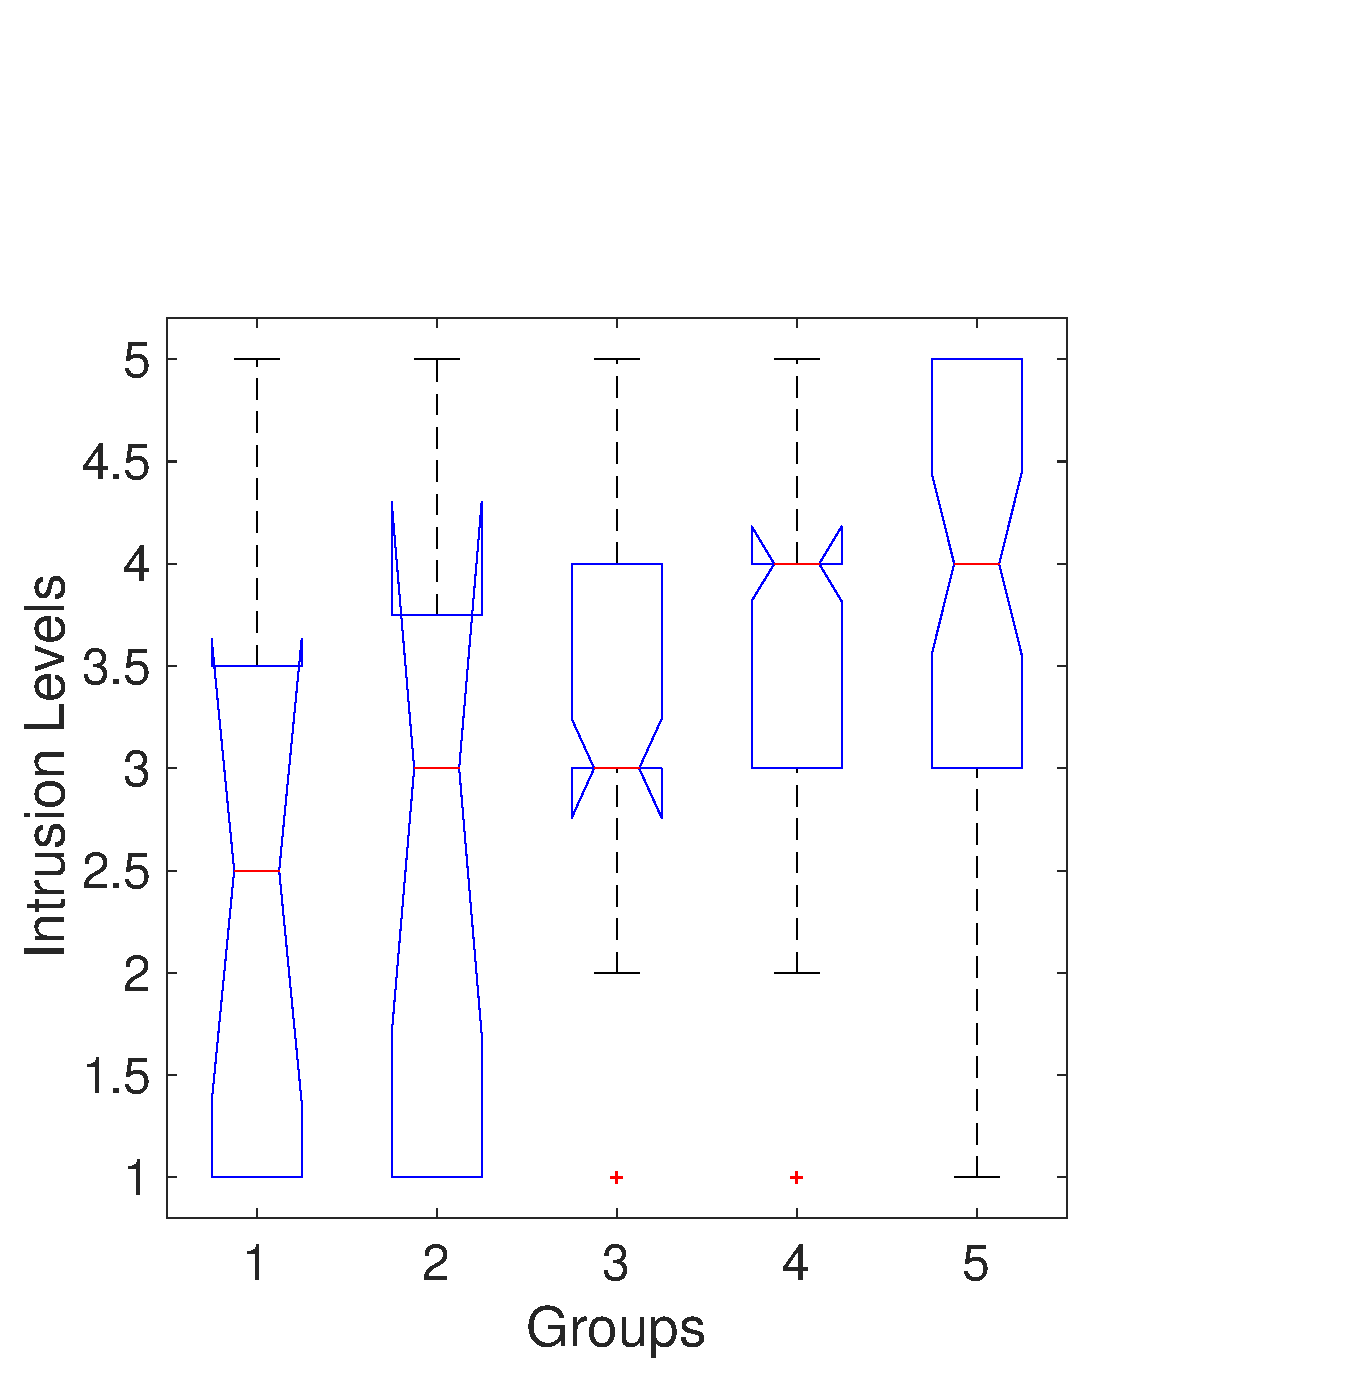
\includegraphics[width=0.47\linewidth]{./images/nav_box}}
%%\caption{Mean and Variance of Groups}
%%\label{fig:st3}
%%\end{figure}
%%
%%In the above, the various intrusions and their relationships with their sub-features was examined. If there was a constant relationship between both, categorization of sub-features in the computational model would be redundant. The above shows that categorizations of sub-features is still essential to the computational model since the data above is not sufficient to make claims about the relationships. In the future, deploying this survey with a larger more representative population can help reduce the number of categorization questions in the model and perhaps even eliminate the categorizations all together. It could also aid to construct better incentivizing mechanisms.
%
\section{Findings from the Experiment}

%The social experiment described in chapter \ref{exp} took place using 9 participants. Out of the total 3 days of the experiment, 3 of the participants did not answer data requests on day 2 and 3. The mobile application ran successfully on all participants phones even after being switched off. All data was successfully recorded on the server. Participants were not paid but were asked to behave like they were paid, so results might skew from the ideal scenario. A trial was run to see if the application created works and to get user feedback on the usability. Additionally, using the data collected on the server, the relationship between data sharing and incentives is examined. 

An emulation of the social experiment explained in Chapter \ref{exp} was held with 9 participants. This was done in order to test the working of the mobile application and receive user feedback before the actual experiment, that will be officially held with the ETH Decision Science Laboratory.

The experiment was held for a period of 3 days. Out of the total number of days, 3 participants did not answer requests on day 2 and day 3. Participants were not monetarily incentivized during the emulation of the experiment, but were asked to think of the incentives indicated in the application as real incentives they will receive. This might cause a deviation from the ideal scenario where users are paid for their participation while examining the results. The mobile application ran successfully on all participating phones even after being switched off. All data was successfully recorded on the server. Using the data collected on the server, the relationship between data sharing and incentives is examined.

\begin{table}[h!]
  \centering
  \caption{Average Score Obtained in the Experiment}
  \label{tab:score}
  \begin{tabular}{ccc}
    \toprule
    Day&Privacy&Cost \\
    \midrule
	1&56.43\%&7.75\\
	2&40.17\%&9.29\\
	3&47.97\%&8.80\\
\bottomrule
  \end{tabular}
\end{table} 

Table \ref{tab:score} shows the average privacy and cost obtained by the users for each day of the experiment. It is observed that the privacy metric is higher on the first day than on day 2 and 3. Furthermore it is also observed that the cost metric is higher on day 2 and day 3 than day 1.
It can be inferred that users have decreased their privacy in order to obtain more cost on day 2 and 3.

\begin{figure}[htp]
\subtop[Improve Privacy and Credit Button\label{fig:button_pri}]{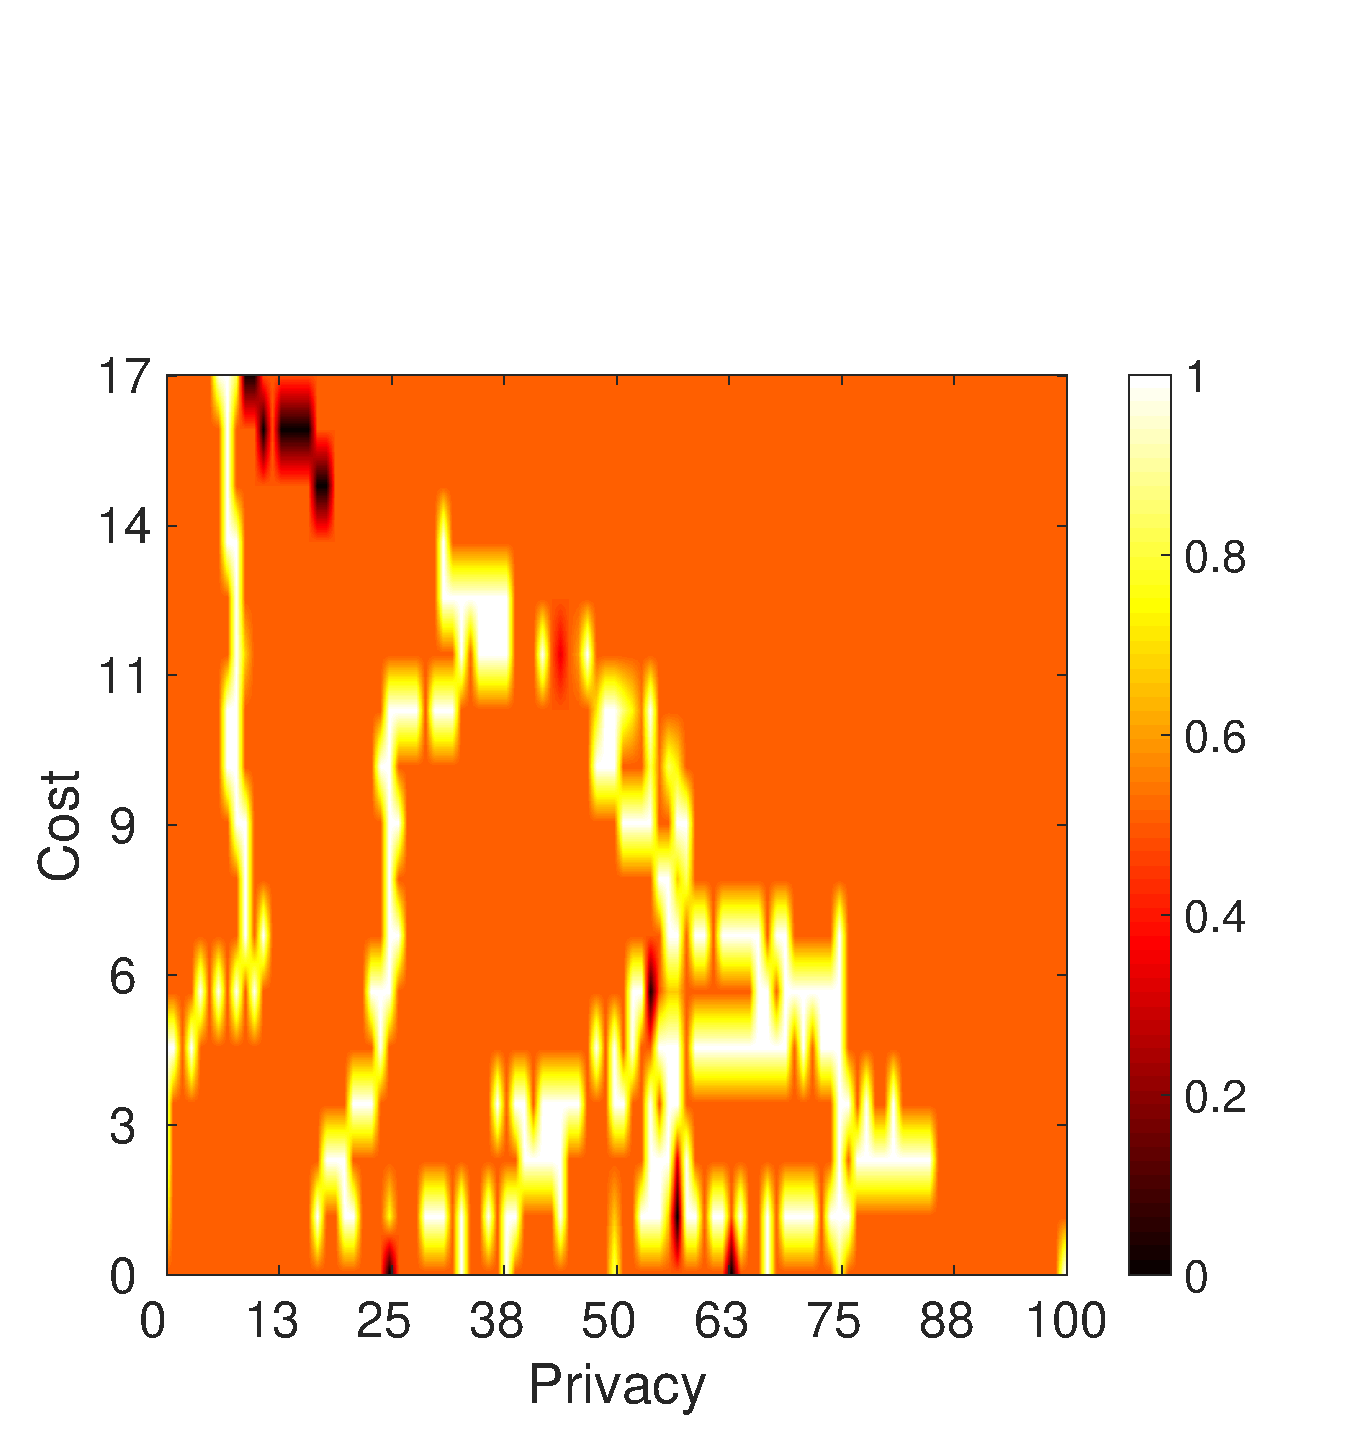
\includegraphics[width=0.5\linewidth]{./images/heatmap_all_days_button}}
\hspace{1em}
\subtop[Actual improvements in Cost and Privacy\label{fig:actual_pri}]{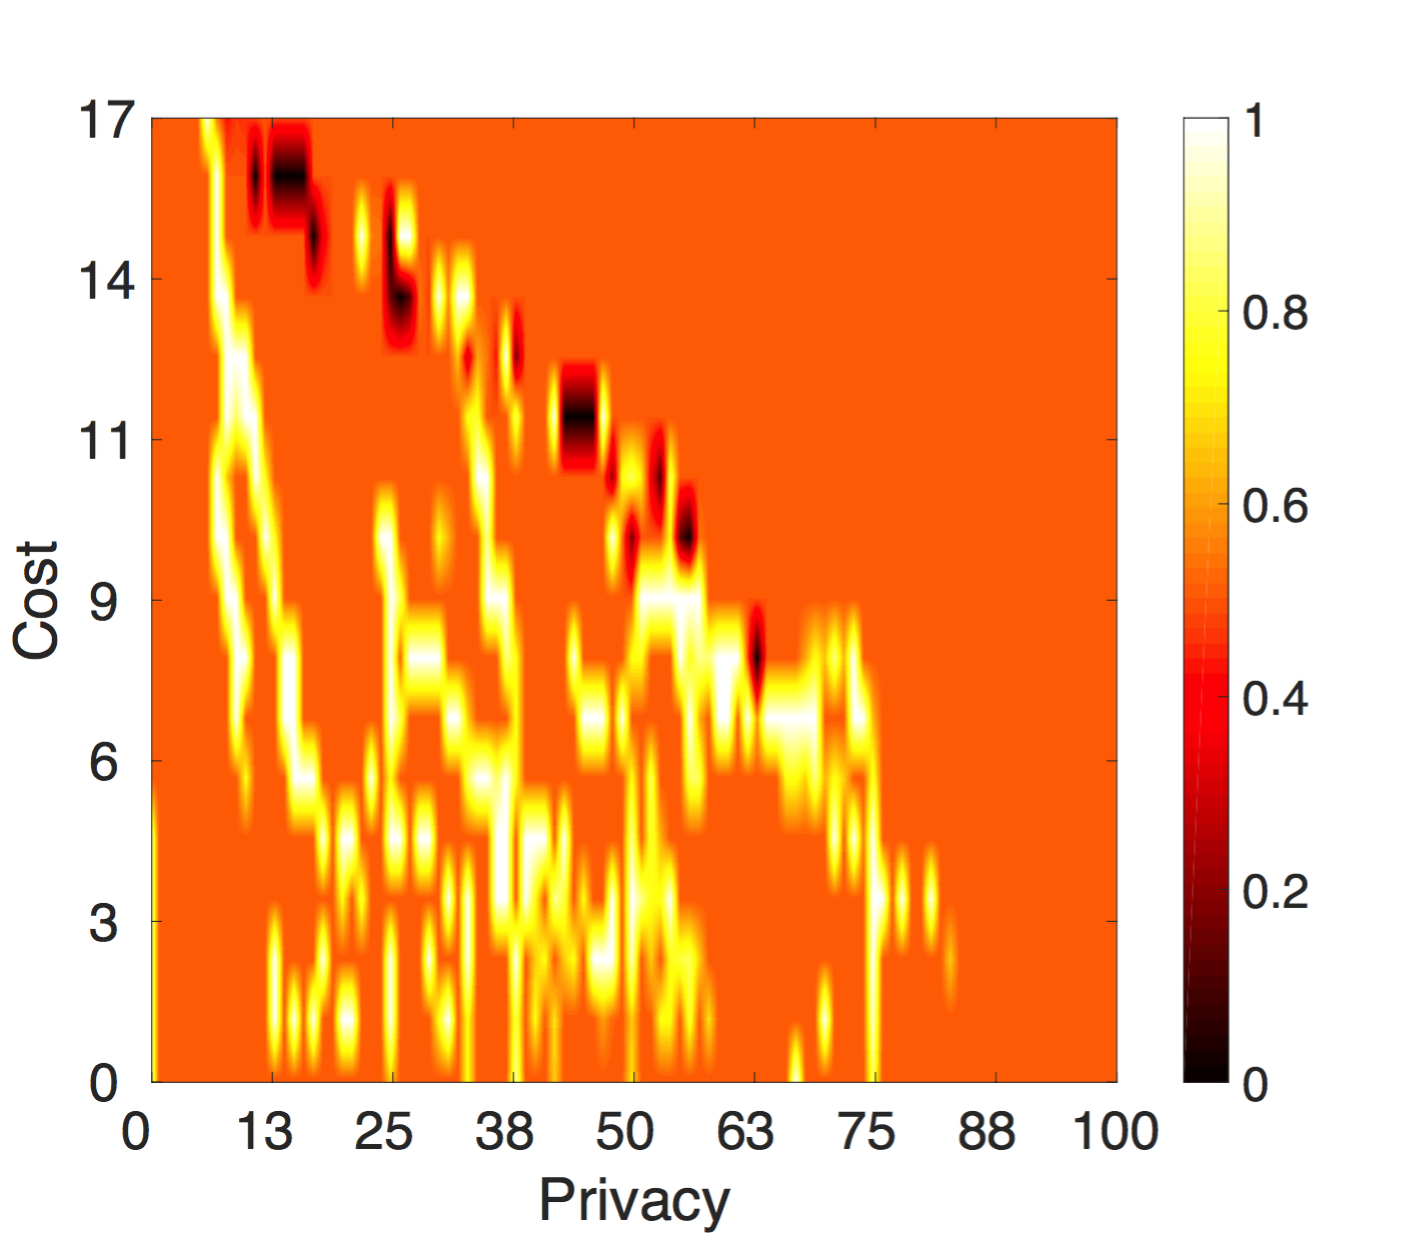
\includegraphics[width=0.5\linewidth]{./images/heatmap_all_days_privacyimprovement}}
\caption{Table Schemas}
\label{fig:st3}
\end{figure}

Figure \ref{fig:button_pri} depicts the of the user clicking on the improve privacy or improve credit button for every possible cost and privacy metric value obtained in the experiment from all participants. Probability values closer to 1 depicts that the user probability of clicking on the improve credit button is highest. Similarly, probability value of 0 depicts that the user's likelihood of clicking on the improve privacy button is highest. The figure depicts that users have higher probabilities of clicking on the improve privacy button when they have a high cost metric and a low privacy metric.

Figure \ref{fig:actual_pri} depicts the probability of an increment in the cost or privacy metric for every possible cost and privacy metric value obtained in the experiment. Probability values closer to 1 depicts the user's likelihood of choosing an option for a data request that will increase the cost metric. Similarly, probability value of 0 depicts the user's probability of choosing an option for a data request that will increase the privacy metric. When Figures \ref{fig:button_pri} and \ref{fig:actual_pri} are observed together, it is seen that when the probability that users click on the improve credit button is high, users clicking on an option for a data request that improves their cost metric is also high. It is also observed that in some areas where the probability of clicking on the improve button is high, Figure \ref{fig:actual_pri} shows that users have a high probability of clicking on an option for a data request that improves their privacy metric. It could be due to the fact that even tough users have more intentions to improve their cost metric as seen before, the ultimate decision could possibly lie on the data request presented whether they will click on an option that will increase the cost or privacy metric.

%Figure \ref{fig:button_pri} depicts for every possible cost and privacy the probability of whether users clicked on the privacy button or credit button. The darker color indicates high probability for clicking on the privacy button (0), a light yellow indicates a higher probability for for clicking on the credit button (1) and the orange depicts the probability of clicking on both buttons equally (0.5). It is observed that probability of users to click on the improve privacy button is very close to when they have no privacy at all and a very high cost. This shows that users are more interested to improve their cost than the privacy metric. 
%
%Similarly, figure \ref{fig:actual_pri} depicts for every possible cost and privacy the probability of whether users actually improved their privacy or their credit rather than just wanting to. The darker color indicates high probability for improvement in privacy (0), a light yellow indicates a higher probability for improvement in credit (1) and the orange depicts the probability of an equal improvement in both metrics (0.5). It is observed that the probability of users incrementing their credit is much higher than their privacy just like in the last figure. Users are interested in improving their privacy when they have sufficient cost
%and their privacy is becoming lower.
%
%Figures \ref{fig:button_pri} and \ref{fig:actual_pri} are now compared. As observed in \ref{fig:button_pri}, users click on the privacy button close to when they have almost no privacy but it is also observed that they improve their privacy even after clicking on the improve credit button as seen in \ref{fig:actual_pri}. This can be attributed to the fact that users were not comfortable giving data for the data requests that appeared, even tough the intentions were to obtain more credit. This means that they were not incentivized enough for those data requests.

\begin{figure}[ht!]
\centering
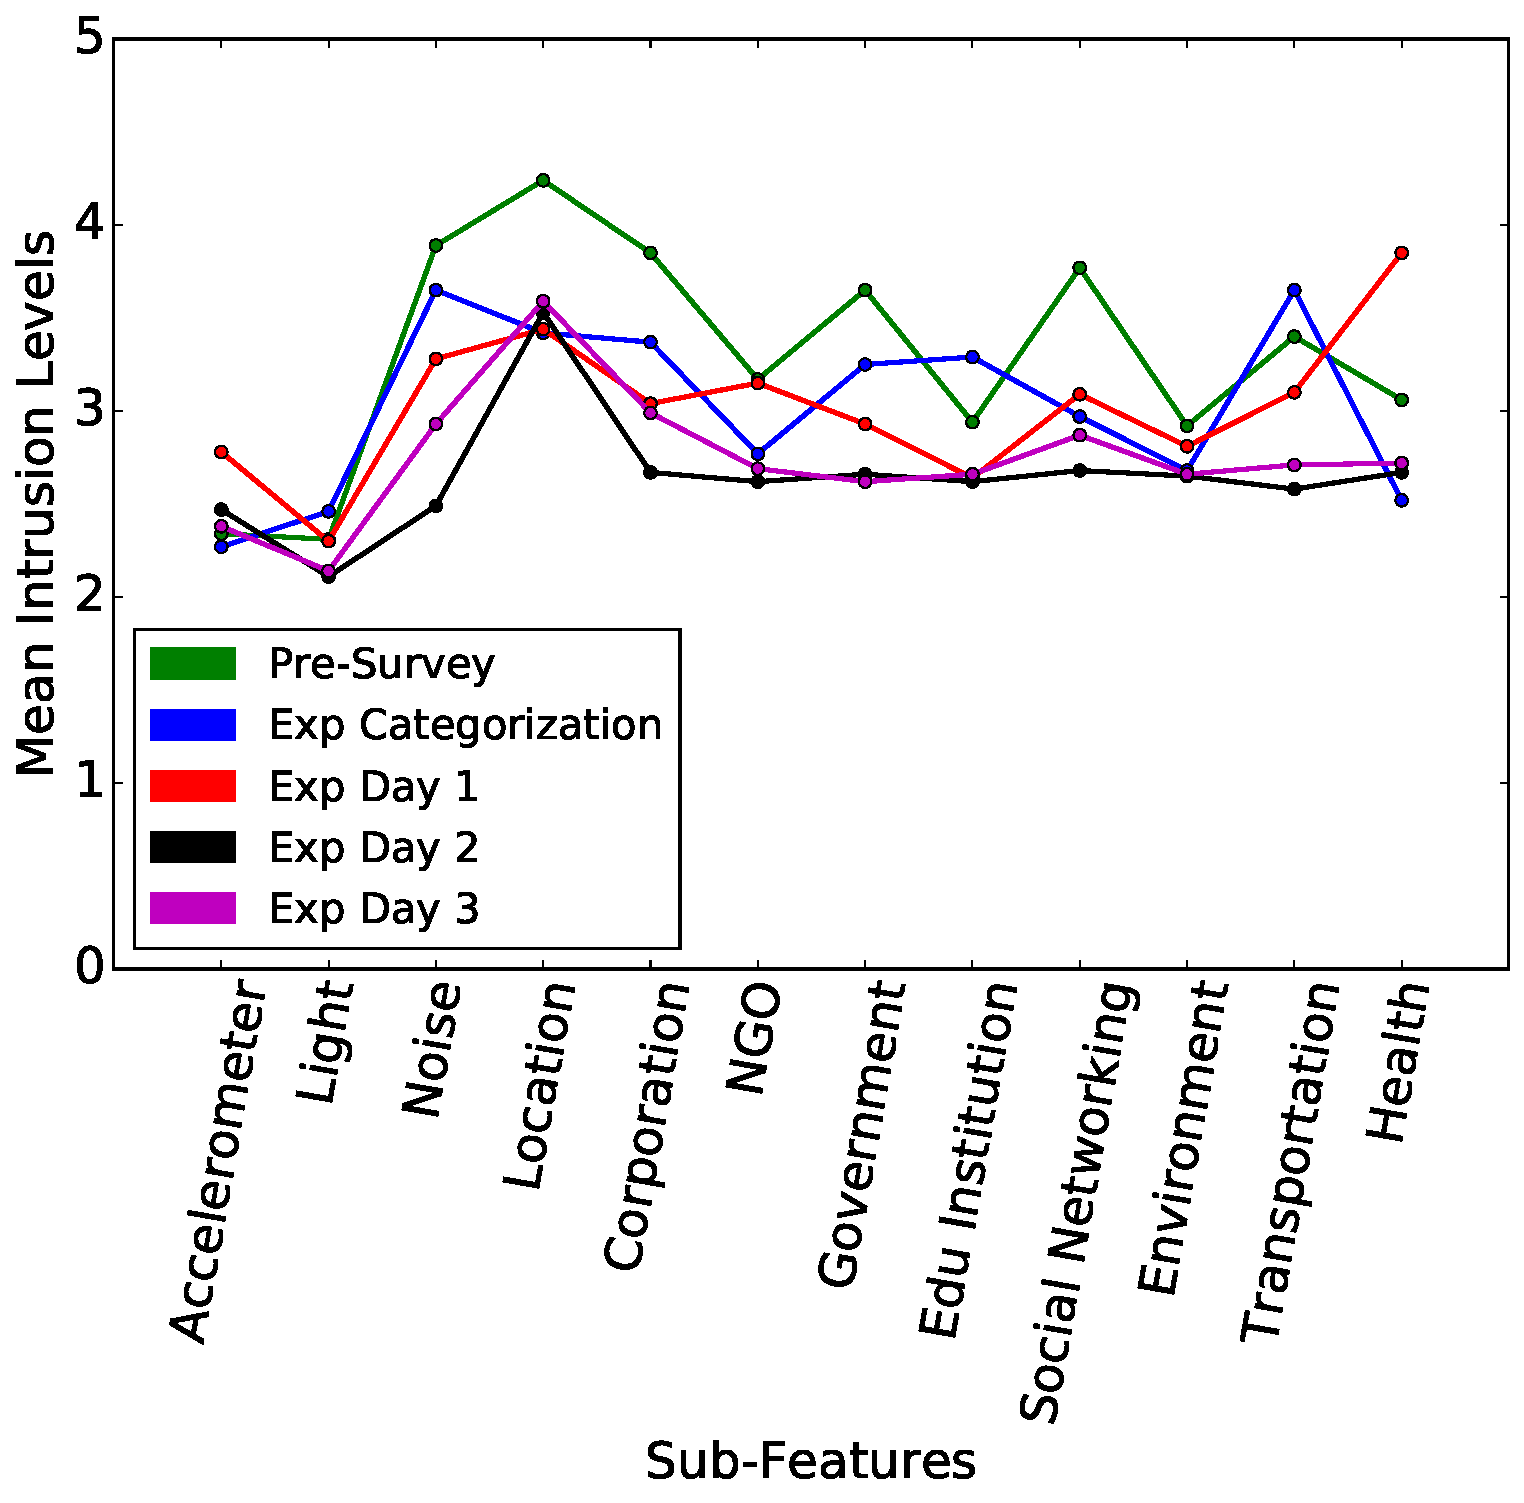
\includegraphics[width=0.6\textwidth,keepaspectratio]{./images/all_sub_mean}
\caption{Mean Privacy Intrusion Levels for Sub-Features}
\label{fig:sum_mean}
\end{figure}

Figure \ref{fig:sum_mean} depicts the mean of the privacy intrusion levels assigned to the sub-features in the pre-survey and experiment categorization. It also depicts how much data was shared for each sub-feature during the experiment on day 1, day 2 and day 3. As it can be seen, there is a difference in the mean privacy intrusion levels assigned during the pre-survey and during the experiment categorization for some sub-features. This is perhaps due to the low number of participants in the experiment.

Additionally, it is observed that for all sub-features, the privacy level chosen for data requests during day 1 of the experiment is much higher than on day 2 and day 3. This is indicated by the day 1 line being much higher than the lines day 2 and day 3. This shows that users have chosen to improve their cost metric on day 2 and day 3.

%The figure \ref{fig:sum_mean} depicts the mean of privacy intrusion levels assigned to the sub-features in the pre-survey, experiment categorization,
%experiment day one, experiment day two and experiment day three. The green and blue lines correspond to the pre survey results and the categorization of sub-features during the experiment. As it is seen, they both carry similar values for every sub-feature on the x-axis. Differences can be attributed to the differences in the sizes of the populations of both samples. 
%
%
%The red line corresponds to day one of the experiment, the black and magenta line to day two and three of the experiment respectively. It is observed that users have been incentivized for most sub-features to share more data on day two and day three than day one except for the location sensor, where giving incentives slightly increased the privacy of the data shared. This can be attributed to the fact that users were aware of how much of their data was being shared with the privacy metric displayed and became more privacy concerned. Additionally, they could have found the incentives insufficient. For the stakeholder education, it is seen that users do not share more data on day 2 or day 3 than day 1. This can be due to the fact that users have already shared a bigger amount of data on day 1 and were not incentivized enough to share even more on the following days.

\begin{figure}[ht!]
\centering
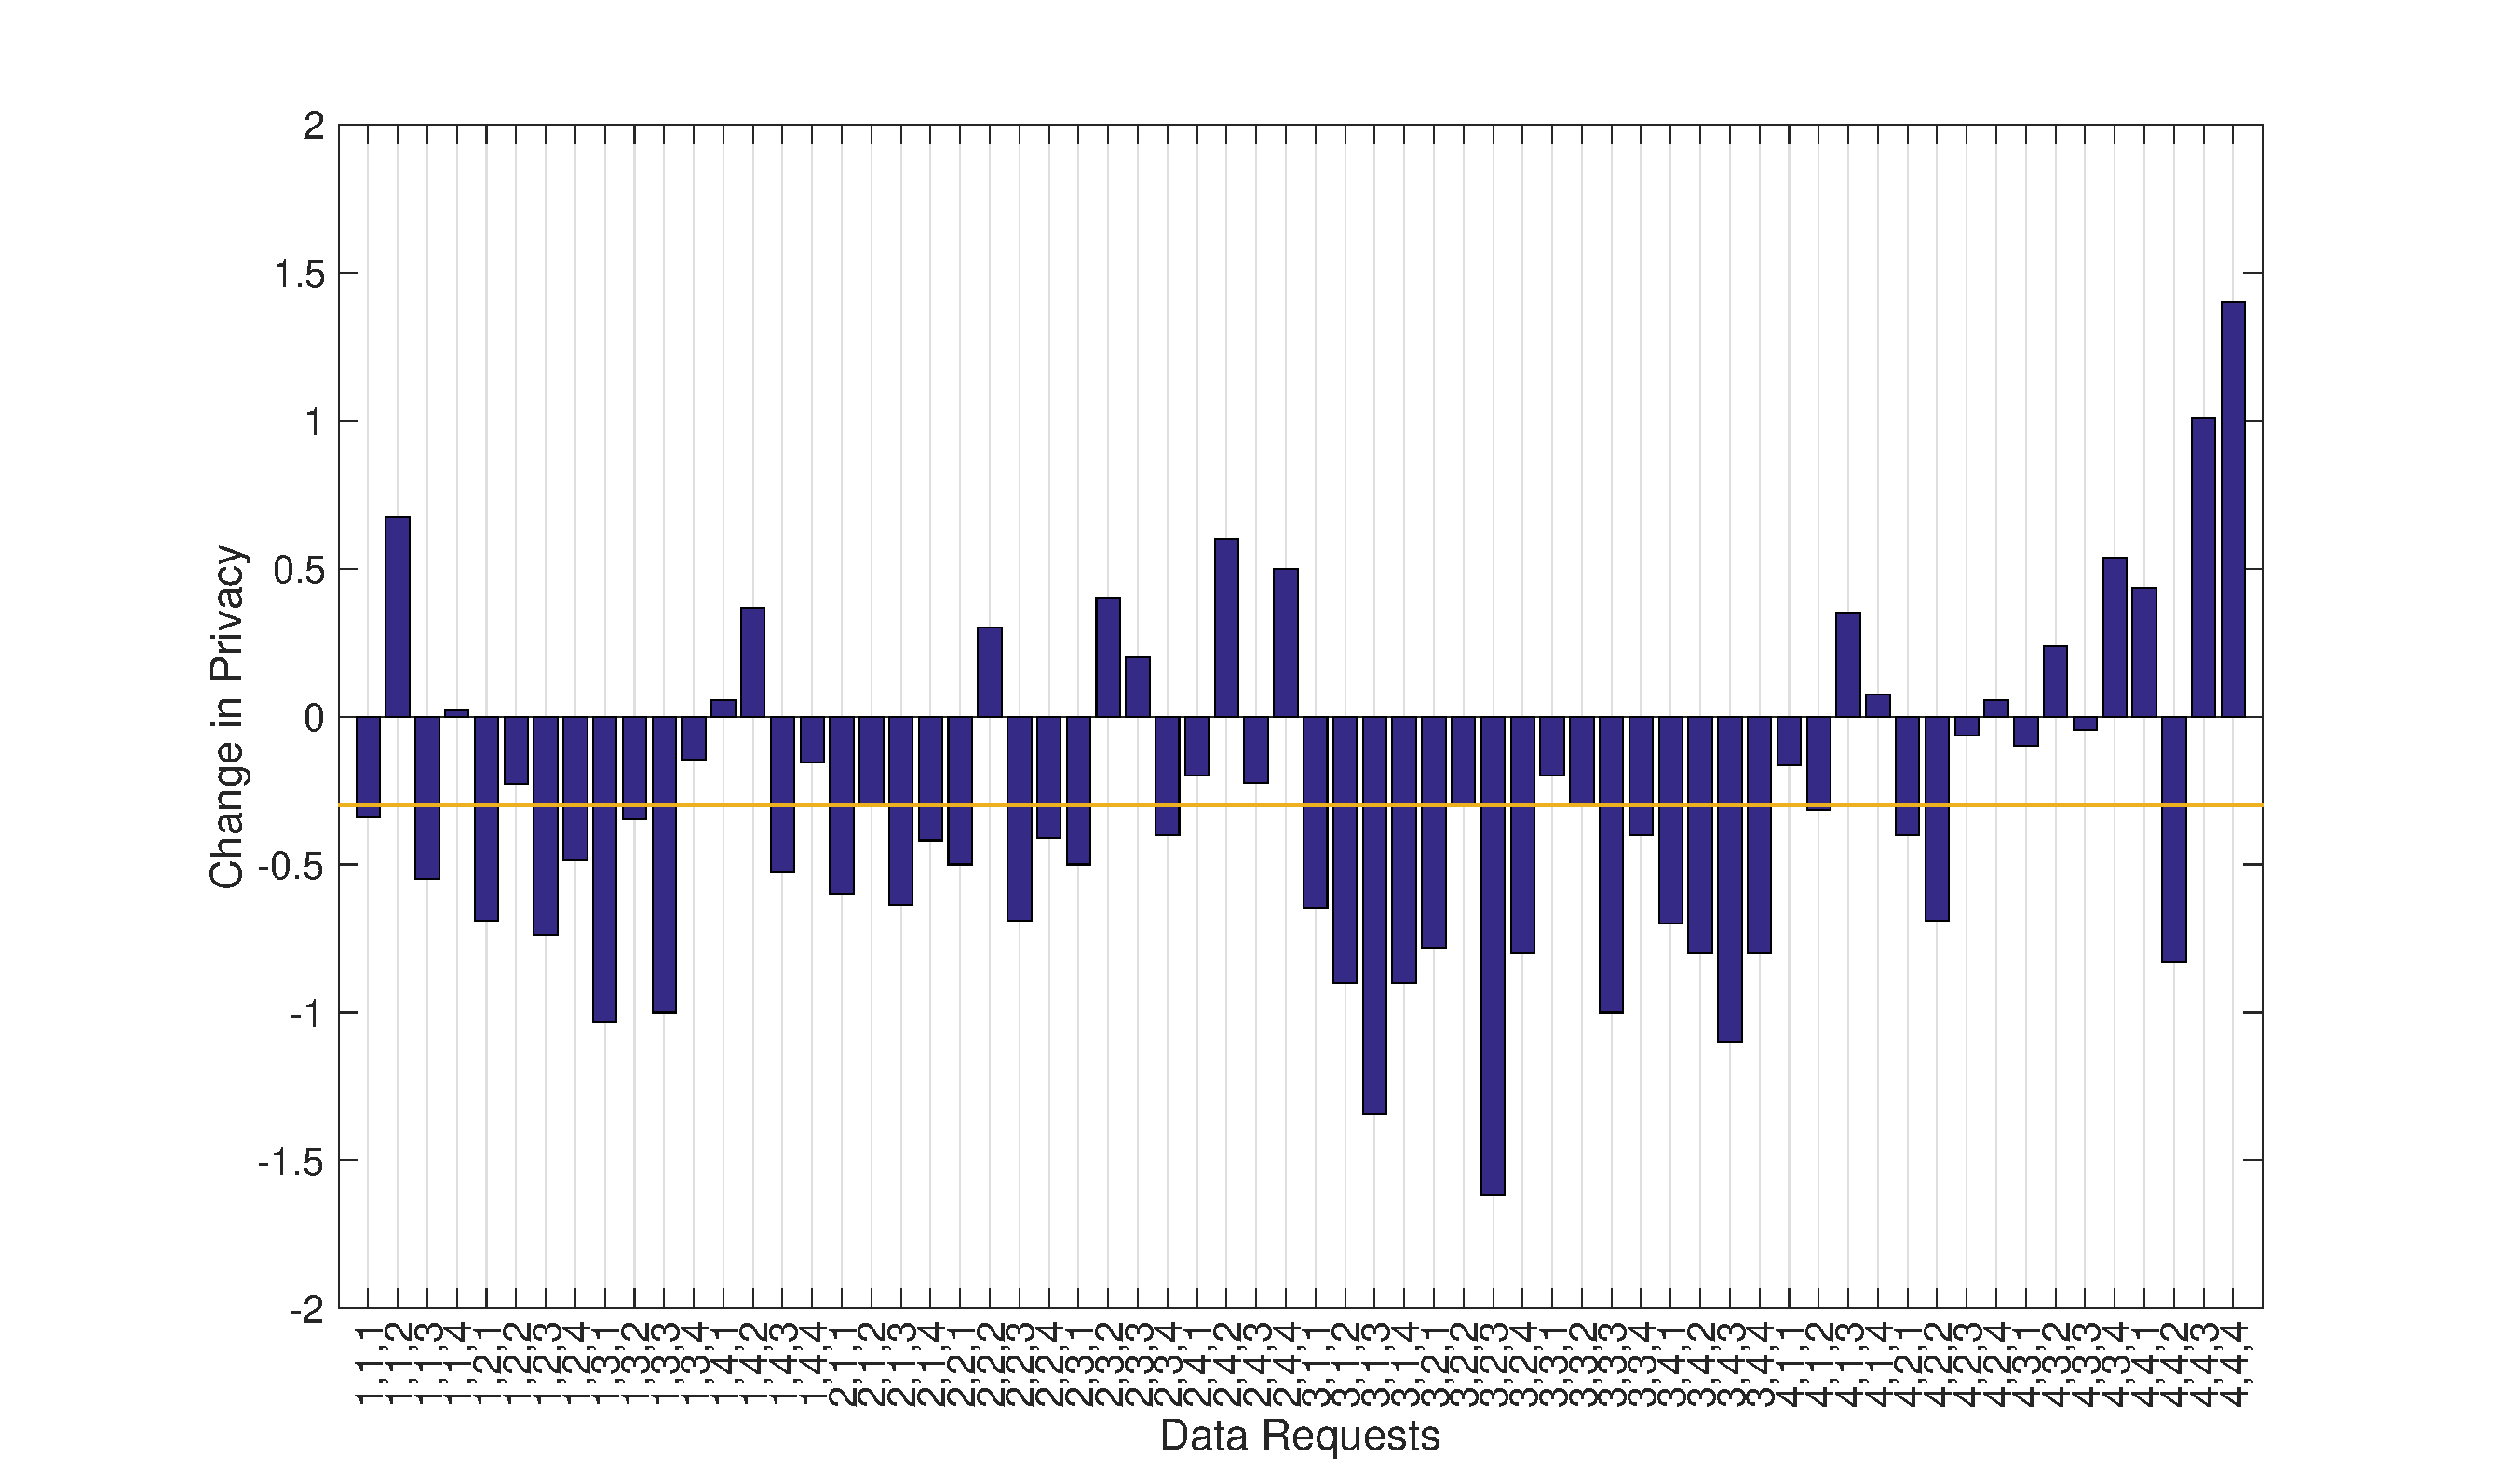
\includegraphics[width=\textwidth]{./images/day2_day1}
\caption{Gain in Privacy Between Day 2 and Day 1}
\label{fig:day2_day1}
\end{figure}

Figure \ref{fig:day2_day1} depicts the gain in privacy for every data request in the experiment between day 2 and day 1. This was obtained by subtracting the responses to data requests on day 2 from the responses to data requests on day 1. If the bars are on the positive side, it indicates that users chose a higher privacy option for that data request on day 2 than on day 1. If the bars are on the negative side, it means that users chose a lower privacy option for that data request on day 2 than on day 1.

It is observed that there are a more bars on the negative side of the graph, indicating that users in general have chosen to decrease their privacy to increase the cost metric. The horizontal line in the graph indicates the mean gain in privacy between day 2 and day 1 for all data requests. The line is on the negative side indicating that users have overall chosen to decrease their privacy and opt to improve the cost metric. 

There are some data requests for which the user has not decreased the privacy such as the data request involving the location sensor, stakeholder education and context transportation. This is perhaps because location sensor is categorized with a privacy intrusion level of 3.42 which is the second most intrusive sensor. Additionally, the context transportation is also categorized with a privacy intrusion level of 3.65 which is the most intrusive context. The stakeholder education is categorized with a privacy intrusion level of 3.29. From the Figure \ref{fig:sum_mean} it can be seen that for day 1, users have already given more data on average for educational institutions. Hence it could be that they were not incentivized enough to give even more data for this stakeholder than they already had. Putting all the points above together could be the reason why data request (4,4,4) has a bar on the positive side of the figure. Similar reasonings can be applied to other data request with an increase in privacy rather than decrease.

\begin{figure}[ht!]
\centering
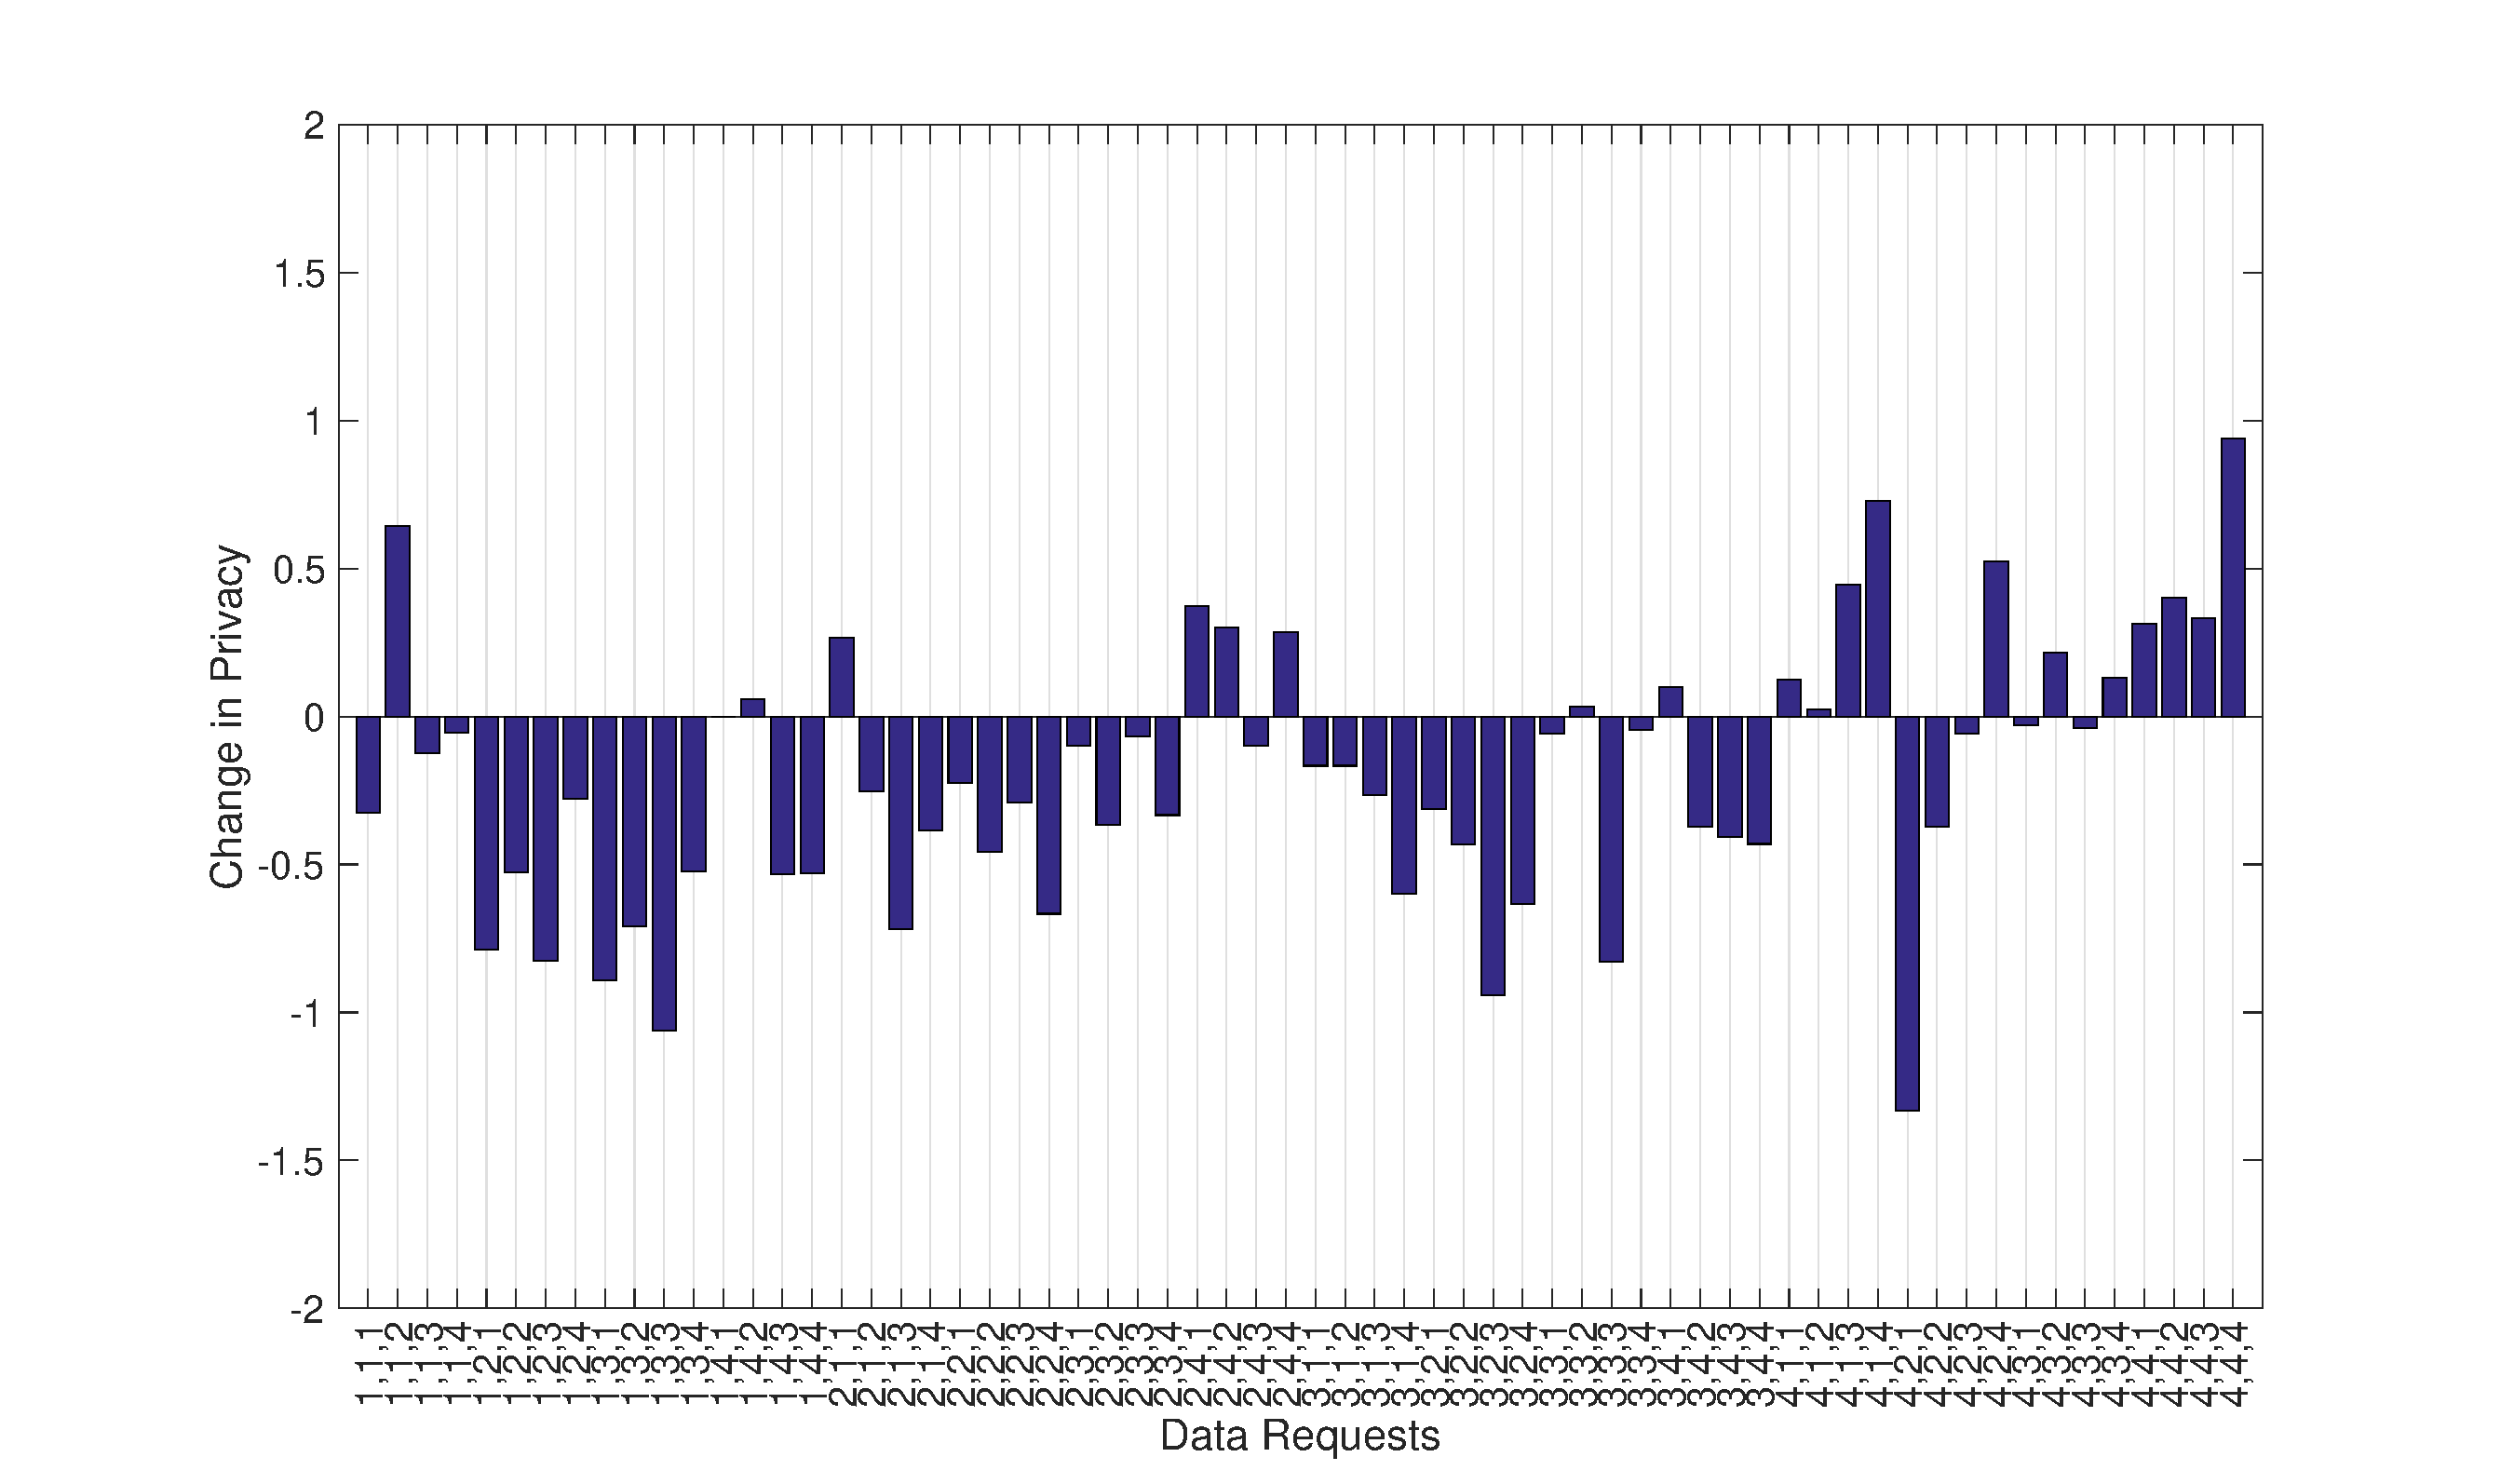
\includegraphics[width=\textwidth]{./images/day3_day1}
\caption{Gain in Privacy Between Day 3 and Day 1}
\label{fig:day3_day1}
\end{figure}

Figure \ref{fig:day3_day1} depicts the gain in privacy for every data request in the experiment between day 3 and day 1. This was obtained by subtracting the responses to data requests on day 3 from the responses to data requests on day 1. If the bars are on the positive side, it indicates that users chose a higher privacy option for that data request on day 3 than on day 1. If the bars are on the negative side, it means that users chose a lower privacy option for that data request on day 3 than on day 1.

It is observed that there are more bars on the negative side than the positive side hence this means that users have shared more data on day 3 than day 1 which means they chose to improve their cost metric over the privacy metric. The horizontal line shown in the figure depicts the average gain in privacy which is on the negative side. This shows that overall they have decreased their privacy level for data requests on day 3 compared to day 1. There are some data requests for which users have shared less data than on day 1, this could be due to the fact that users were not incentivized enough for these data requests.

\begin{figure}[ht!]
\centering
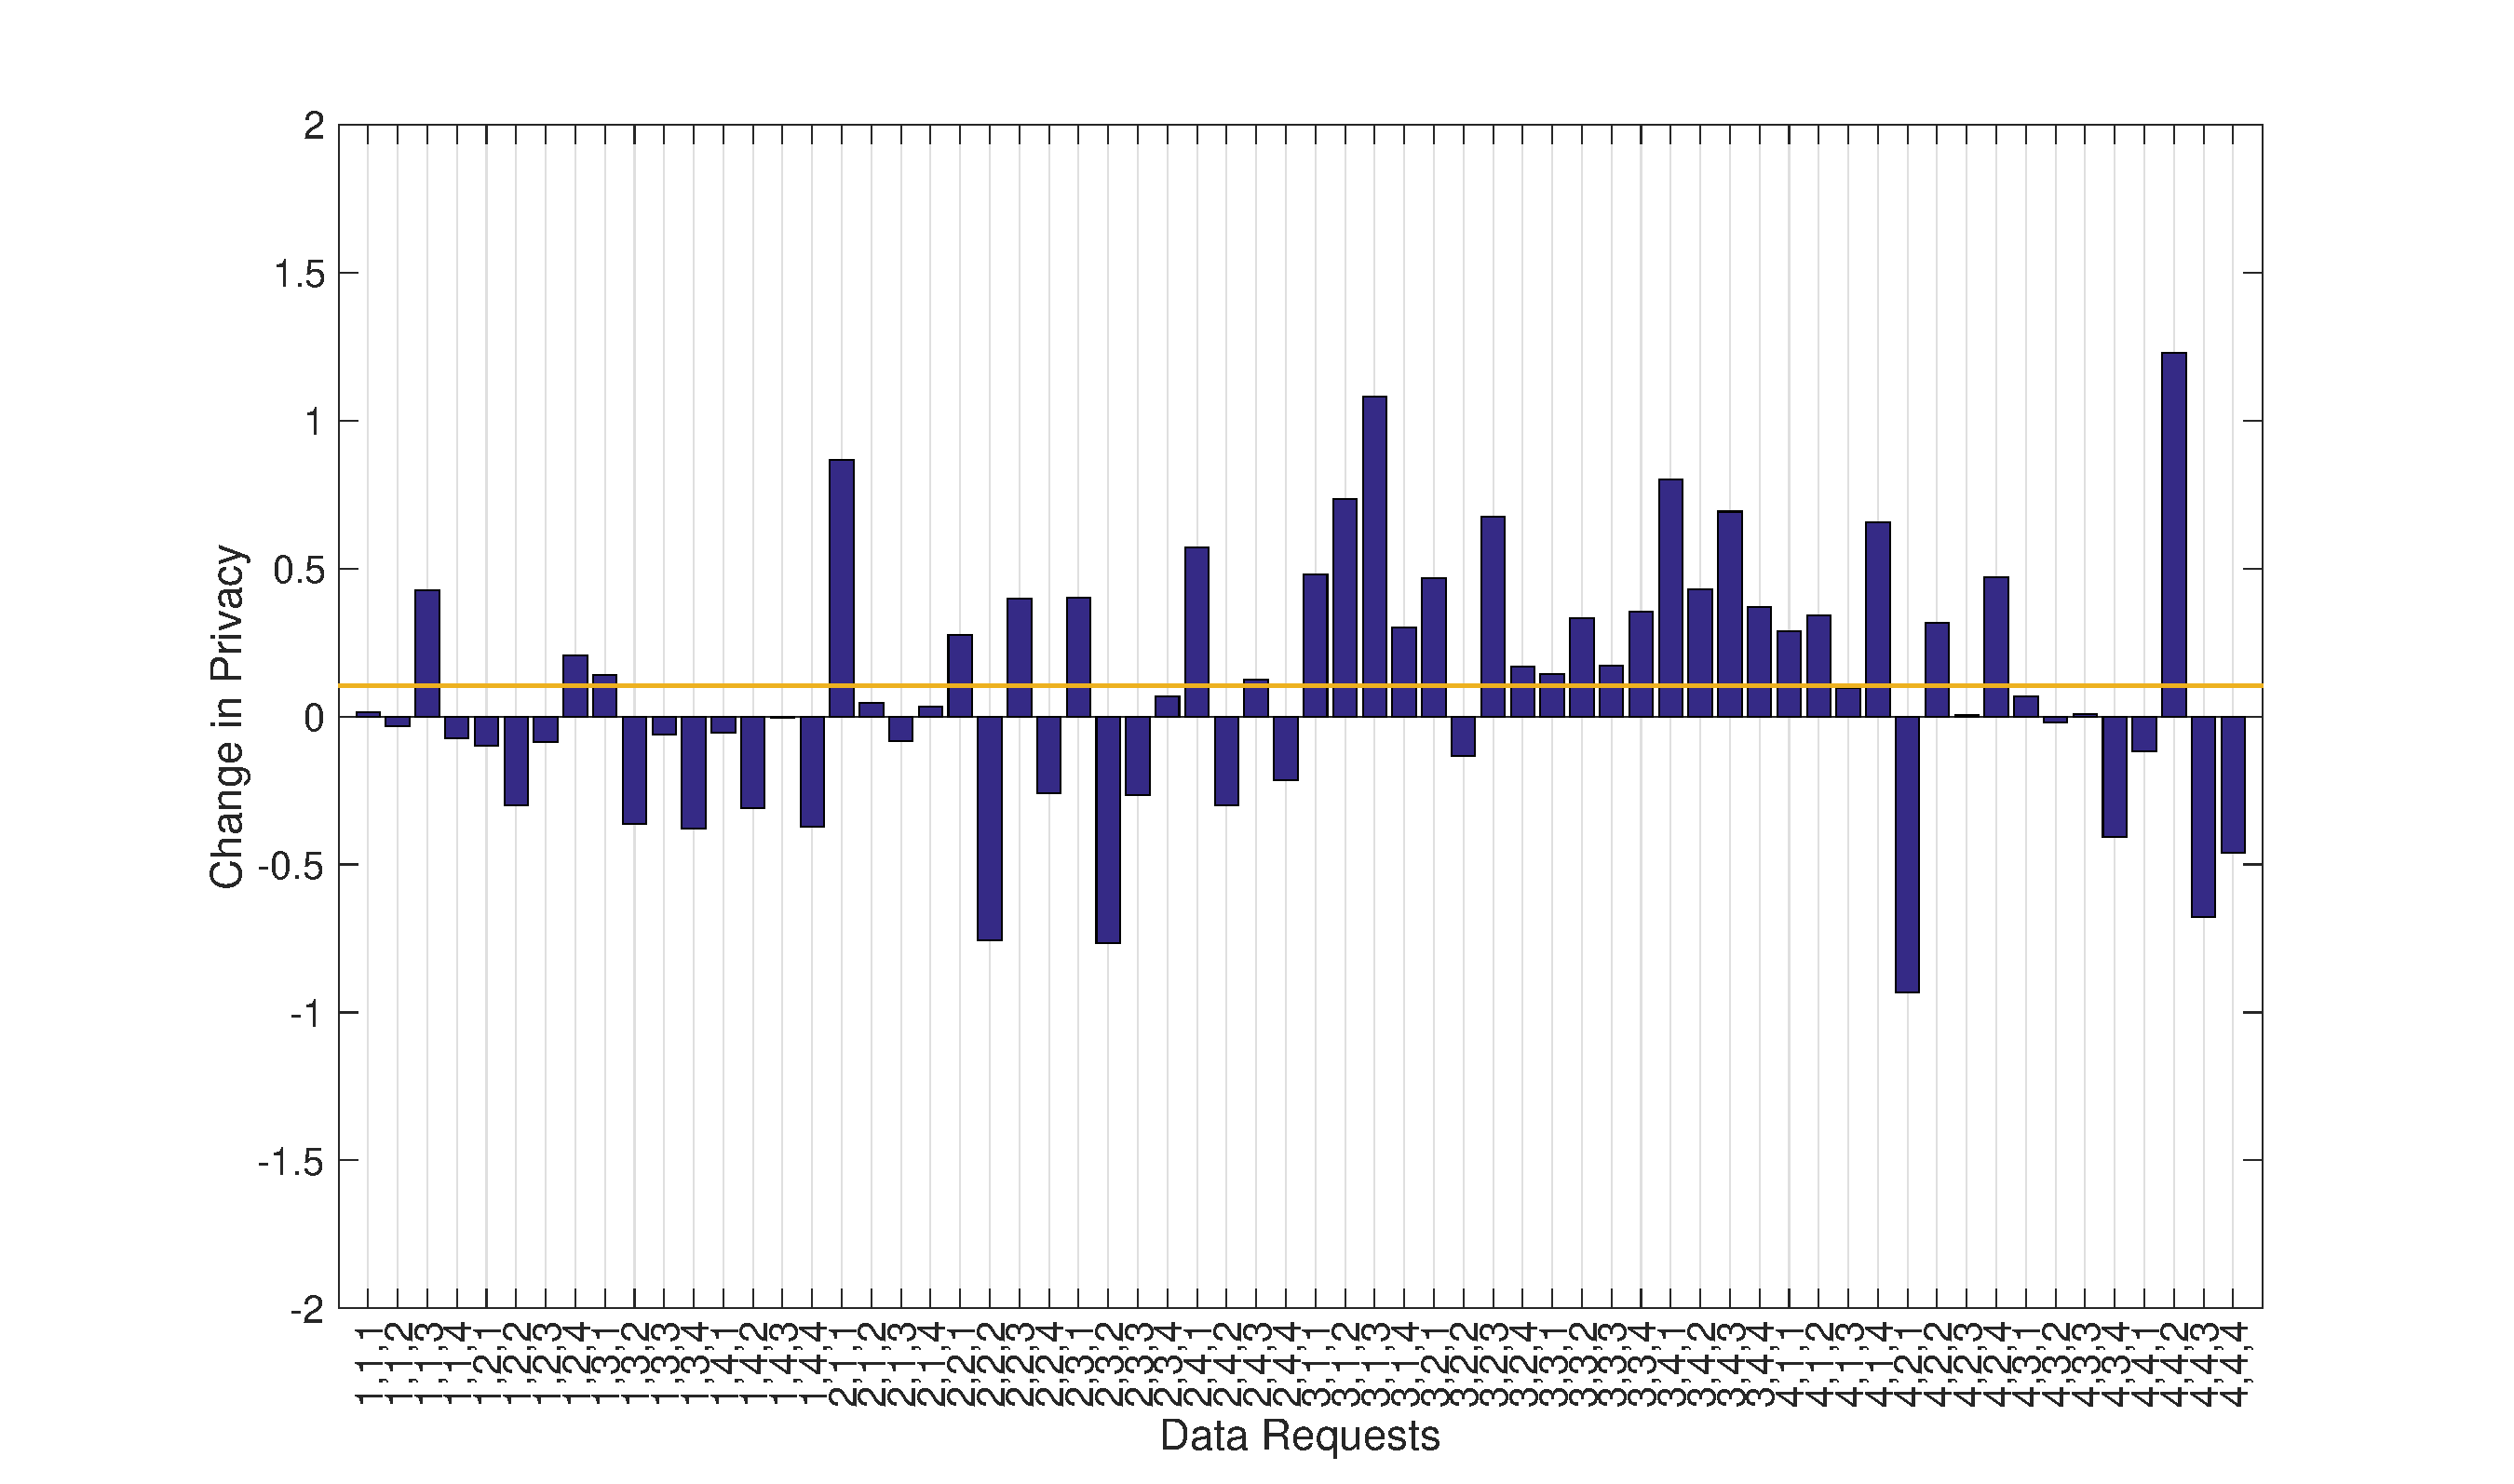
\includegraphics[width=\textwidth]{./images/day3_day2}
\caption{Gain in Privacy Between Day 3 and Day 2}
\label{fig:day3_day2}
\end{figure}

Figure \ref{fig:day3_day2} depicts the gain in privacy for every data request in the experiment between day 3 and day 2. This was obtained by subtracting the responses to data requests on day 3 from the responses to data requests on day 2. If the bars are on the positive side, it indicates that users chose a higher privacy option for that data request on day 3 than on day 2. If the bars are on the negative side, it means that users chose a lower privacy option for that data request on day 3 than on day 2.

As it is observed, the horizontal line which indicates the average gain in privacy is on the positive side which means that users have on average increased their privacy on day 3 compared to day 2. Additionally, it can be seen that there are more bars on the positive side. This could be due to the fact that users expected more rewards on day 3, or that they became more privacy aware as they used the application due to the privacy metric.

%The individual increment or decrement of privacy for every data request between incentive and non-incentive days are now examined. Figure \ref{fig:day2_day1} depicts the gain in privacy for day 2 compared to day 1. On day 2, incentives were given for data requests whereas in day 1 no incentives were given. The x-axis depicts each data request with a sensor identifier, a stakeholder identifier and a context identifier. For detailed explanation as to which feature belongs to which unique identifier please refer to the section \ref{struct}. Since on an average, the contexts were categorized as 3.26 and more intrusive than the rest, they play a bigger role in the model for the incentive assignments than sensors and stakeholders which are categorized as low intrusion sub-features. 
%
%For the accelerometer, it is observed that for corporations for environment and health contexts users did not share more data than day 1. This can be due to the fact that they were categorized on average as 2.68 and 2.52 respectively, hence these requests were not assigned enough incentives to share more data. Educational institutions were rated second most intrusive with value of 3.29, the contexts social networking and environment were assigned intrusions of 2.97 and 2.68 respectively. For social networking the data request associated with it could have been assigned insufficient incentives whereas for the environment context it was assigned a lower categorization level and hence could have had a very low incentive assigned compared to the rest of the data requests. Furthermore, since the accelerometer was assigned a category of 2.27 which is low in intrusion, the data requests were assigned lower incentives.
%
%For the light sensor, it is observed that users gave more data for corporations due to its high categorization compared to the others of 3.37, since it was assigned much higher cost and users were incentivized. For the context environment we see that users did not share their data which is categorized as 2.68. But for the health context categorized as 2.52 they shared more data. This can be attributed to the fact that they find environment more intrusive than the health context and users were not incentivized enough or that the sample obtained is not representative. For the noise sensor, which is rated categorized the most intrusive of all as 3.65, users shared more data than on day 1. This can be due to the fact that it was assigned a much higher incentive than for the other sensors.
%
%The location sensor is assigned a category of 3.42 which is the second most intrusive sensor after the noise sensor, there are a lot of requests for which more data was not shared. This can be due to insufficient increment in incentives for this sensor compared to the other sensors for requests. Health context was categorized as 2.52 as the least intrusive context and users were not incentivized enough to share location data for lower incentives. For the stakeholder educational institution, users have shared less data except for the context environment. The reasons can be that users already shared a lot of data on day one and the incentives given were not enough to incentivize them to share more on day two.
%
%It is seen that for most data requests the privacy is negative which means users chose lower summarization levels to gain more credit. Similarly, figure \ref{fig:day3_day1} depicts the gain in privacy for day 3 compared to day 1. In day 3, incentives were given for data requests whereas in day 1 no incentives were given. Here as well it is seen that users have chosen to improve their credit compared to day 1. 
%
%On day 3 \ref{fig:day3_day1}, more of the users are responding to incentives as it is seen that there are lesser bars on the positive side of privacy compared to day 2. This can be because users were getting used to the application interface on day 2 and were more explorative to see changes in privacy and credit metrics. Additionally, it is also observed that the bars in the negative side in day 3 are smaller than day 2. This can be because users may be expecting even higher rewards for day 3 of the experiment than day 2, but still wanted to improve their credit.
%
%For the accelerometer, it is seen that the environment context did not provide sufficient incentives for users to share to educational institutions and corporations. Corporation stakeholder was rated intrusive and probably the incentives given were not sufficient. For the educational institution stakeholder it can be seen in figure \ref{fig:sum_mean} users already shared more data on day 1 and hence were not incentivized enough to share even more on day three. For the light sensor, the context social networking was categorized as intrusive but still did not incentivize users to share more data than day 1. For the stakeholder educational institution, and for the context transportation users shared more data this could be due to the fact that transportation was considered intrusive and hence assigned higher incentives. 
%
%%%In the light sensor, for the corporation and educational institutions users did not share more data for the social networking context. 
%For the sensor noise, users shared more data than day one for all stakeholders and contexts one except for the educational institution stakeholder for the purpose of social networking. For the location sensor the data requests containing the health context more data was not shared. This can be due to the fact that health context is assigned a lower incentive due to its lower categorization of 2.52. The very intrusive transportation context assigned a 3.65 categorization of intrusion, users did not share more data to the intrusive stakeholders corporation and for educational institutions due to the fact that more data was already given on day one. For the context environment, since it is categorized as lowly intrusive with 2.68, enough incentives were not given and did not motivate users to share more of their sensor data than on day one. Lastly, for stakeholder educational institution and corporations which considered intrusive, users did not share more data for the context social networking because they found the sensor, context and stakeholder combination intrusive.
%
%To summarize, we found that users did give away more data for day 2 and day 3 than on day 1. On day 2, it is seen that some data requests for which features are considered non-intrusive during categorization are being given lesser with incentives than without. This could be due to the fact that users could have been explorative during the first day, with the metrics and the application itself. On day 3, it is observed that responses to data requests are more consistent with the categorization of the features. Small inconsistencies of the responses with the categorizations can be attributed to the fact that the population of the experiment was 6 people for day 2 and day 3, hence even if one person answers dramatically differently it affects the overall mean.

\section{Findings from the Exit Survey}

8 fully filled entries were recorded from the exit survey. No incentives were awarded to participate in this survey. The following paragraphs will present the findings obtained from the survey.

\begin{figure}[htp]
\subtop[User evaluation of application quality\label{fig:exit_6}]{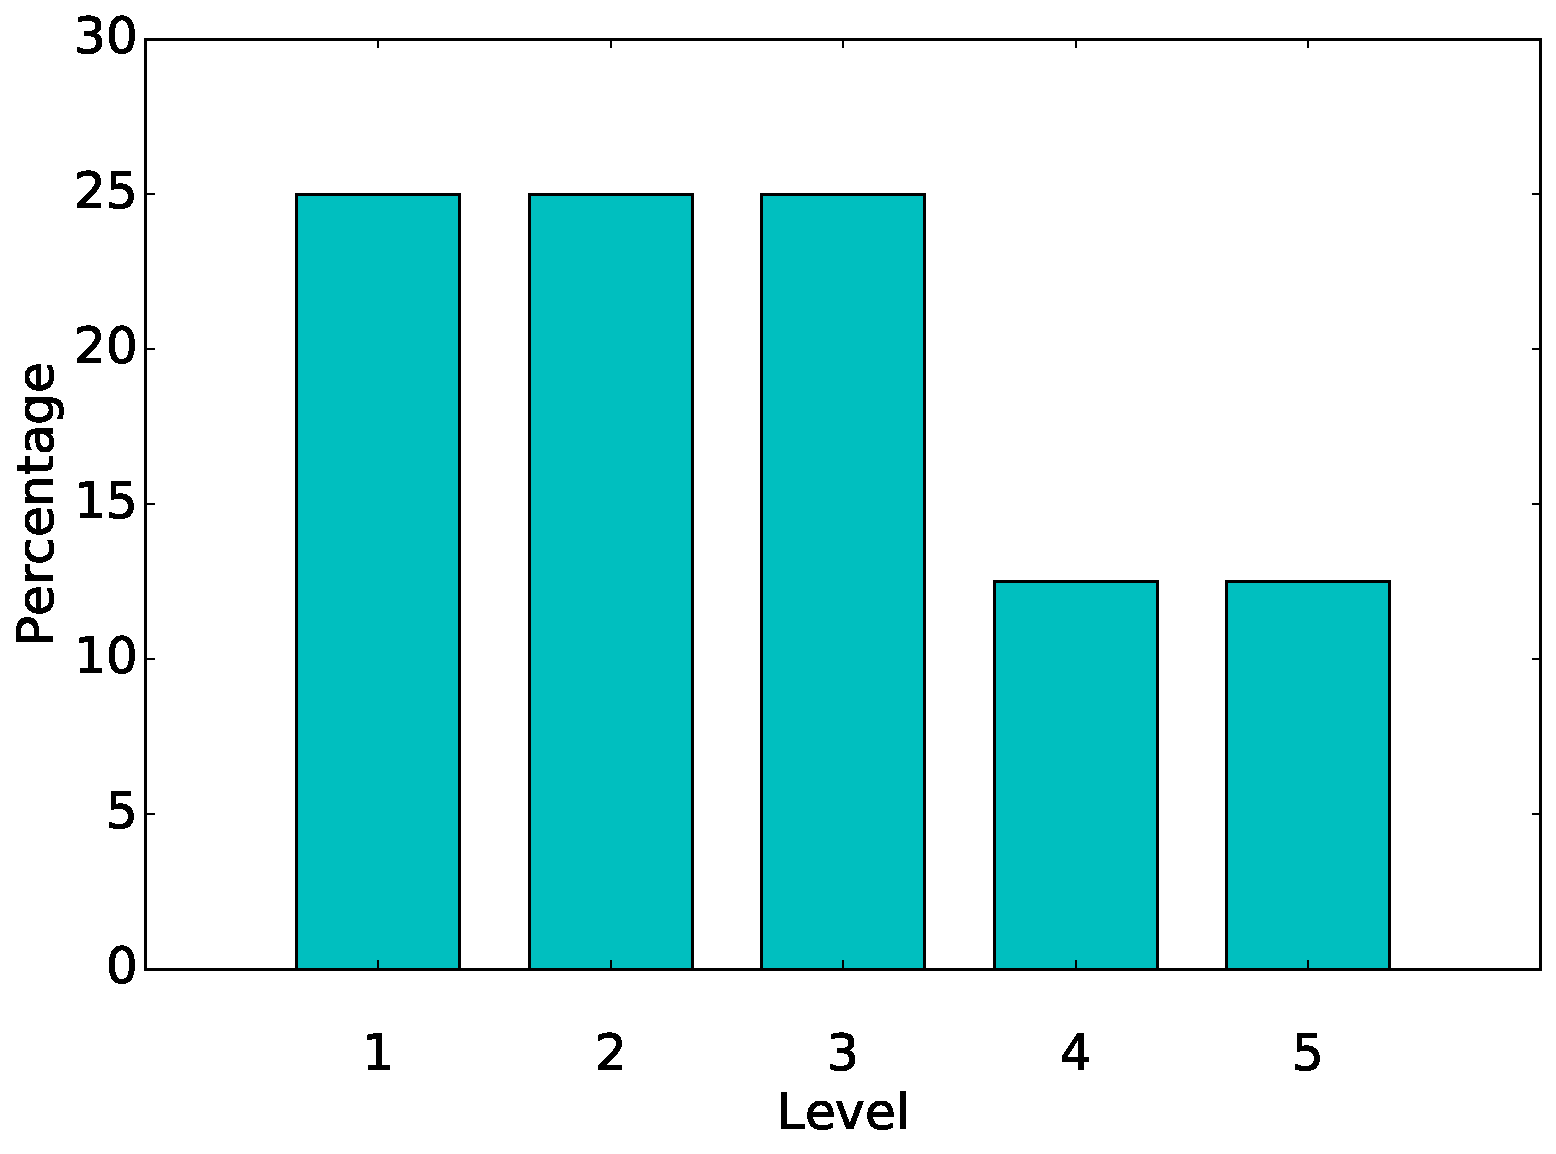
\includegraphics[width=0.45\linewidth]{./images/exit_app_quality}}
\hspace{1em}
\subtop[User evaluation of the ease of use of the application\label{fig:exit_5}]{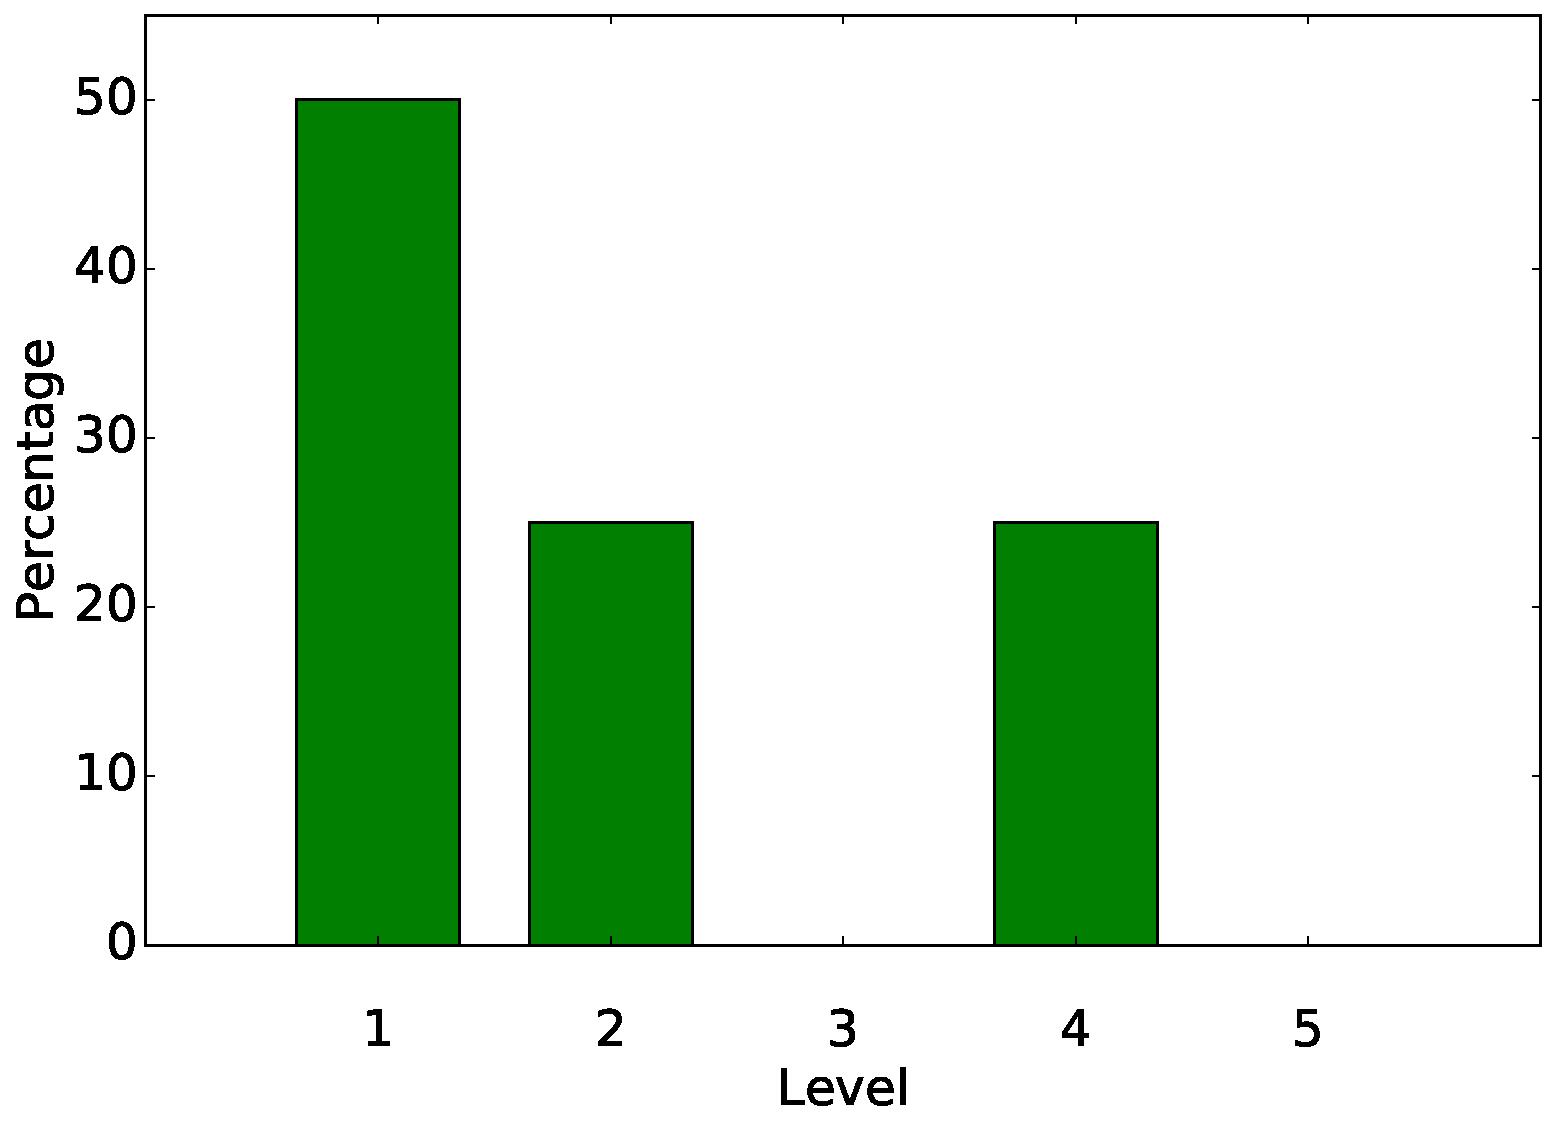
\includegraphics[width=0.45\linewidth]{./images/exit_ease_use}}\newline
\centering
\subtop[User evaluation of various features of the application\label{fig:exit_7}]{\includegraphics[width=0.45\linewidth]{./images/exit_eval_features}}
\caption{General user evaluation of the application}
\label{fig:st3}
\end{figure}

Figure \ref{fig:exit_6} depicts the user ratings for the quality of the application. 1 stands for "Extremely good" and 5 stands for "Extremely bad". As observed in the figure, 75\% of users think of the application quality to a level of neither good or bad and above (level 1,2 and 3).

Figure \ref{fig:exit_5} depicts the user ratings for the ease of use of the application. 1 stands for "Extremely easy" and 5 stands for "Extremely difficult". It is observed that 75\% of users find the application to be at least somewhat easy to use (level 1 and 2).

Figure \ref{fig:exit_7} depicts the user rating of the battery life, performance and speed, colors of the application, formulation of the data requests, content of the data requests, number of data requests, frequency of notifications and their overall opinion. A rating of 1 indicates that the user is "Extremely dissatisfied" and a rating of 5 means that the user is "Extremely satisfied". It is seen that users are most satisfied with the performance, application colours and with the application overall with ratings of 3.63, 3.38 and 3.13 respectively. Users are less satisfied with the battery life, questions formulation, content of the questions and the number of questions with ratings of 2, 2.5, 2.25 and 2.13 respectively. 

\begin{figure}[htp]
\subtop[User evaluation of the comprehension of features\label{fig:exit_9_1}]{\includegraphics[width=0.45\linewidth]{./images/exit_metrics_useful}}\hspace{1em}
\subtop[User evaluation of the usefulness of features\label{fig:exit_9_2}]{\includegraphics[width=0.45\linewidth]{./images/exit_metrics_comp}}\newline
\subtop[User evaluation of the privacy\label{fig:exit_12}]{\includegraphics[width=0.45\linewidth]{./images/exit_privacy_questions}}
\hspace{1em}
\subtop[User evaluation of rewards satisfaction\label{fig:exit_13}]{\includegraphics[width=0.45\linewidth]{./images/exit_cost_questions}}\newline
\centering
\subtop[User evaluation of the cost\label{fig:exit_14}]{\includegraphics[width=0.45\linewidth]{./images/exit_cost_questions_14}}
\caption{User evaluation of cost and privacy}
\label{fig:st3}
\end{figure}

Figure \ref{fig:exit_9_1} depicts the user ratings for the comprehension of the total cost, total privacy, rewards for each option of a data request, privacy for each option of a data request and the indicator of options (orange recommendation box). A rating of 1 indicates that the user is "Extremely dissatisfied" and a rating of 5 means that the user is "Extremely satisfied". It is seen that users have a better understanding of the total cost and rewards for each option of a data request with ratings of 3.38 and 3.25 respectively than the total privacy, privacy for each option of a data request and the indicator of options (orange recommendation box) with ratings of 2.88, 3.13 and 3 respectively.

Figure \ref{fig:exit_9_2} depicts the user ratings for the usefulness of the total cost, total privacy, rewards for each option of a data request, privacy options for a data request and the indicator of options (orange recommendation box). A rating of 1 indicates that the user is "Extremely dissatisfied" and a rating of 5 means that the user is "Extremely satisfied". It is seen that users find the total cost and rewards for each option of a data request most useful with ratings of 3.38 and 3.25 respectively than the total privacy, privacy for each option of a data request and the indicator of options (orange recommendation box) with usefulness ratings of 3, 2.88 and 2.88 respectively.

Figure \ref{fig:exit_12} depicts the user responses to "if the experiment makes them more aware about the privacy of their data", and "if the privacy-preservation of their data deserves the sacrifice of their rewards". A rating of 1 indicates "Definitely not" and a rating of 5 means "Definitely yes". Experiment making users more aware about the privacy of their data receives a rating of 3 and the privacy-preservation of data deserving the sacrifice of their rewards receives a rating of 3.13. This shows that users are willing to sacrifice their privacy.

Figure \ref{fig:exit_13} depicts the user responses to the satisfaction of users to the total obtainable rewards (30 Chf) and the satisfaction of users to the rewards they obtained out of the total obtainable rewards. A rating of 1 indicates "Definitely not" and a rating of 5 means "Definitely yes". It is seen that users are not satisfied with the total rewards of 30 Chf for 2 bidding days indicated by a rating of 2.25. Users indicate that they are more satisfied about the rewards they obtained out of the total possible rewards with a rating of 2.88. 

Figure \ref{fig:exit_14} depicts the user responses to if rewards convince users to share data, if rewards convince users to share more data than without rewards, if rewards make users more privacy aware, if rewards make users aware about the value of their data and if rewards deserve the sacrifice of the privacy of their data.  A rating of 1 indicates "Definitely not" and a rating of 5 means "Definitely yes". Users agree more that rewards convince them to share more of their data, rewards make them more aware of the privacy of their data and that rewards make them aware about the value of their data to a rating of 3, 3.25 and 3. Users gave a rating of 2.75 and 2.75 to rewards convincing them to share data and rewards deserving the sacrifice of the privacy of their data. 

\begin{figure}[htp]
\subtop[User experiment interest\label{fig:exit_25}]{\includegraphics[width=0.45\linewidth]{./images/exit_dropout}}
\hspace{1em}
\subtop[User FairDataShare portal visit\label{fig:exit_29}]{\includegraphics[width=0.45\linewidth]{./images/exit_visit_fds}}\newline
\centering
\subtop[User evaluation of the technical problems faced\label{fig:exit_27}]{\includegraphics[width=0.45\linewidth]{./images/exit_tech_probs}}
\caption{User responses to experiment interest, FairDataShare portal visit and technical problems faced}
\label{fig:st3}
\end{figure}

Figure \ref{fig:exit_25} shows whether users wanted to drop out of the experiment at any point of time. As it is seen, 75\% of users said "no" and 25\% of users said "yes". Some of the reasons stated to drop out of the experiment are \textit{"battery drain"} and \textit{"it got boring after a point"}.

Figure \ref{fig:exit_29} shows whether users visited the FairDataShare portal at any point of time in order to see what sensor data has been collected from them. As observed, 75\% of users said "yes" and 25\% said "no".

Figure \ref{fig:exit_27} shows the percentage of users who suffered from technical problems. Users did not face problems of the application crashing or problems of the application being slow. The problems 66.67\% of users faced is the drain of their battery charge. This is due to the fact that sensor data is constantly collected from them as a background service in the application and this is a battery intensive task. 16.67\% of users faced problems of network connectivity. There is no indication that the application is the cause of the network connectivity problem. 16.67\% faced problems of the application interface freezing. Finally, 16.67\% of users faced other problems. When looking in to this further, the "other" problem was due the fact that the privacy and cost metrics did not change as the user re-answered data requests. This is due to the fact that if the user repeatedly answers the same data requests again with the same responses, the metrics will not change. The metrics only change when the user re-answers a data request with a difference response, otherwise same rewards and privacy are obtained for this data request and this does not change the privacy and cost metrics.
